\documentclass[12pt,letterpaper,onecolumn,openany,oneside]{book}
% Use draft option to be overfull 
% \includeonly{TightBinding,PVP,Appendix_TB_strainedBZ,Appendix_TB_idependence}
% \includeonly{PVP}

%%%%%%%%%%%%%%%%%%%%%%%%%%%%
%%   additional packages  %%
%%%%%%%%%%%%%%%%%%%%%%%%%%%%
\usepackage{graphics,graphicx}         		% Figures
\usepackage{amsmath,amssymb,mathrsfs,bm} 	% Math symbols
\usepackage{tikz}                      		% Fancy drawings
\usepackage{apalike}						% APA like bibliography style

%%%%%%%%%%%%%%%%%%%%%%%%%%%%
%%    Custom Commands     %%
%%%%%%%%%%%%%%%%%%%%%%%%%%%%
\newcommand{\angstrom}{\textup{\AA}}		% Angstrom command

%%%%%%%%%%%%%%%%%%%%%%%%%%%%
%%     Format             %%
%%%%%%%%%%%%%%%%%%%%%%%%%%%%
% Sets the margins--one sided document only odd commands are taken into effect
\usepackage[top=1.5in, bottom=1in, left=1.5in, right=1in]{geometry}
\setlength{\footskip}{.25in}				% Page numbers in footer are positioned bottom margin-\footskip from bottom of page to give 0.75"
\setlength{\headheight}{15pt}				% To avoid an error in fanyhdr
% Note: headers is automatically 1" from top of page like it should be
\usepackage{fancyhdr}						% Custom setup of header and footers which allows number positions to be placed
\usepackage[doublespacing]{setspace}		% Sets double spacing for main textand provides single spacing environment
\usepackage[font=doublespacing]{caption}	% Captions now also double spaced
\usepackage{sectsty}                  		% needed for the \allsectionsfont command
\allsectionsfont{\normalsize}				% Sets all section headers to 12 pt
\usepackage{layout}							% If you use the \layout command in the body of the text the formatting will be shown nicely

% Formatting still to do:
% No journal abbreviations in the bibliography (will have to manually edit :( )

\begin{document}
	\frontmatter							% Preamble
	\fancypagestyle{plain}{					% Must redefine plain otherwise pages with chapter start (TOC, LOF, LOT) will look different
		\fancyhf{}								% all header footer field clear
		\fancyfoot[C]{\thepage}					% page number in right header
		\renewcommand{\headrulewidth}{0pt}		% gets rid of lines that fancyhdr always sticks in
		\renewcommand{\footrulewidth}{0pt}}
	\pagestyle{plain}
	\begin{titlepage}
\begin{center}

  BOSTON UNIVERSITY\\

  \vspace{1mm}

  GRADUATE SCHOOL OF ARTS AND SCIENCES\\

  \vspace{.75in}

  Dissertation\\

  \vspace{.75in}

  \textbf{Manipulating graphene's lattice: Anomalous friction, metastable band gap, and pseudovector potentials}\\

  \vspace{2mm}
  \vspace{.4in}

  by\\

  \vspace{.4in}

  {\bf Alexander L. Kitt}\\

  \vspace{1mm}

  B.S. and B.A., University at Buffalo, 2008\\

  \vspace{-1.5mm}

  M.A., Boston University, 2012

  \vspace{-2.5mm}

  \vfill

  Submitted in partial fulfillment of the\\
  requirements for the degree of\\
  Doctor of Philosophy\\
  2014\\

\end{center}
\end{titlepage}
	\begin{titlepage}	% No page number, next page is page 1

\begin{center}
Approved by
\end{center}

\vspace{1.5in}

\begin{singlespace}
	\noindent
	First Reader\ \ \ \ \  \ \rule{4.7in}{.005in}\\
	\hspace*{1.15in}Bennett B. Goldberg, Ph.D.\\
	\hspace*{1.15in}Professor of Physics \\
	\hspace*{1.15in}Professor of Electrical and Computer Engineering \\
	\hspace*{1.15in}Professor of Biomedical Engineering\\

	\vspace{0.75in}

	\noindent
	Second Reader\ \ \ \rule{4.7in}{.005in}\\
	\hspace*{1.15in}Anna K. Swan, Ph.D.\\
	\hspace*{1.15in}Associate Professor of Electrical and Computer Engineering\\
	\hspace*{1.15in}Associate Professor of Physics\\
\end{singlespace}

\end{titlepage}
	\setcounter{page}{3}					% Sets the page number to 3
	\chapter*{Acknowledgments}
With deep gratitude I thank my advisors Bennett Goldberg and Anna Swan for crafting me into the physicist I am today.
Special thanks to Bennett for giving me the freedom to follow my ideas, and to Anna for having the patience to listen to my latest experimental foible.

Many thanks to my many collaborators.
Specifically I would like to thank the reputable graphene strain theorists Harold Park, Zenan Qi and Vitor Pereira, the brilliant Kekul\'e theorists Claudio Chamon and Tom Iadecola, the masters of helium scattering Michael El-Batanouny and Colin Howard, and the graphene growth gurus at UT Austin Rod Ruoff, Richard Piner, and Ji Won Suk.
Additional thanks go to my lab mates Sebastian Remi, Xuanye Wang, and Jason Christopher and my cohort at BU, especially Alan Gabel, Elsa Abreu, John Ogren, Cory Fantasia, and Kang Liu.

Thanks to the folks at SIF, principally Heitor Mourato, Bob Fazio, and Joe Volho, who routinely made substance out of my imagination.
Special thanks to the late Bob Kingsland, a great teacher who was always able to make me feel at home and at ease-onwards and upwards.

I would like to thank my parents and most loyal fans, Anne Mercier and Greg Kitt, for giving me the traits which carried me through graduate school: An expectation of myself and the confidence to work with my hands.
I would also like to thank my wife's parents, Dede and Stan Colwell, for their acceptance and encouragement.

Most importantly I would like to thank my wife, Jess, for helping me through my N+1 failures.
This could never have happened without her unwavering love and support.

\newpage
	\vspace{-0.2in}

\begin{center}

\textbf{Manipulating graphene's lattice: Anomalous friction, metastable band gap, and pseudovector potentials}\\
 
\vspace{0.2in}

(Order No.\ \ \ \ \ \ \ \ \ \ \ \ \ )\\

\vspace{0.2in}

\textbf{Alexander L. Kitt}\\
Boston University Graduate School of Arts and Sciences, 2014\\
Major Professor: Bennett B. Goldberg, Professor of Physics, Professor of Electrical and Computer Engineering, Professor of Biomedical Engineering\\

\vspace{0.4in}

\textbf{ABSTRACT}

\end{center}

\noindent
Abstract text here, double spaced, 350 words 
	\tableofcontents
	\listoftables
	\listoffigures
	\include{form6_abbreviations} 			% Listed alphabetically


	% Body text
	\mainmatter								% Main text
	\clearpage								% Finishes anything from \frontmatter before switching style
	\fancypagestyle{plain}{					% Must redefine plain otherwise pages with chapter start will look different
		\fancyhf{}								% all header footer field clear
		\fancyhead[R]{\thepage}					% page number in right header
		\renewcommand{\headrulewidth}{0pt}		% gets rid of lines that fancyhdr always sticks in
		\renewcommand{\footrulewidth}{0pt}}
	\pagestyle{plain}
	\chapter{Unmodified band structure\label{chap:TB}}

The linear electronic dispersion of graphene was first published by Wallace\cite{Wallace1947} 57 years before Geim, Novoselov and co-workers spurred graphene research forward with their method of mechanical exfoliation\cite{Novoselov2004}.
Later, in 1984 Semenoff formalized the equivalence between the low energy electrons in graphene and Dirac-Weyl electrons \cite{Semenoff1984}.
Remarkably, the nearest neighbor tight binding approach used by these authors has accurately described the majority of the low energy physics in graphene.
This chapter will follow in the spirit of these derivations with additional emphasis provided to enhance the discussions of the strain induced pseudo vector potential and the phonon induced Kekul\'e transition.

\section{Graphene's lattice and Brillouin zone}
\begin{figure}
	\begin{center}
	{
% Geometry taken directly from my lectures notes on tight binding in graphene
\newcommand{\alat}{1 cm}
\newcommand{\sqth}{1.73205080757}
\newcommand{\Klen}{2 cm}
\begin{tikzpicture}															

	% Graphene lattice, sublattices different colors, nearest neighbor vectors and lattice vectors
	\begin{scope}[xshift=-3.75 cm,>=stealth,
		nnarrow/.style={color=black,very thick, ->},					% Nearest neighbor vectors
		B/.style={circle,draw=blue!50,fill=blue!20,
			thick,minimum size=2 mm,inner sep=0pt}, 					% A sublattice dots
		A/.style={circle,draw=orange!70,fill=orange!40,
			thick,minimum size=2mm,inner sep=0pt},						% B sublattice dots
		el1/.style={x radius=.3*\alat,y radius=.85*\alat},				% Style for the ellipse
		el2/.style={dashed,thick,draw=black!75}]						% Style for the ellipse draw

		%This scope is clipped to limit the drawn lattice to a square
		\clip (-3.9cm,-4.38cm) rectangle(3.9cm,3cm);
		% Draw the lattice
		\foreach \ip in {-3,-2,...,3}
			\foreach \im in {-3,-2,...,3}
			{
			\node at (\ip*\sqth*\alat/2-\im*\sqth*\alat/2, \ip*\alat*3/2+\im*\alat*3/2+\alat/2) [A] {};
			\node at (\ip*\sqth*\alat/2-\im*\sqth*\alat/2, \ip*\alat*3/2+\im*\alat*3/2-\alat/2) [B] {};
			}

		% Draw the nearest neighbor vectors
		\draw[nnarrow] (60:\alat*\sqth)++(-30:\alat)++(0,-\alat/2) -- +(270:\alat) node[anchor=north     ]{$\vec{\delta}_1$};
		\draw[nnarrow] (60:\alat*\sqth)++(-30:\alat)++(0,-\alat/2) -- +( 30:\alat) node[anchor=south west]{$\vec{\delta}_2$};
		\draw[nnarrow] (60:\alat*\sqth)++(-30:\alat)++(0,-\alat/2) -- +(150:\alat) node[anchor=south east]{$\vec{\delta}_3$};
		
		% Draw the lattice vectors
		\draw[nnarrow] (240:2*\sqth*\alat) --node[circle,anchor=north west]{$\vec{a}_+$} +( 60:\sqth*\alat) ;
		\draw[nnarrow] (240:2*\sqth*\alat) --node[circle,anchor=north east]{$\vec{a}_-$} +(120:\sqth*\alat);

		% Ellipses around two atom basis
		\draw[el2] (240:2*\sqth*\alat) +(  0,0          ) ellipse[el1];
		\draw[el2] (240:2*\sqth*\alat) +( 60:\sqth*\alat) ellipse[el1];
		\draw[el2] (240:2*\sqth*\alat) +(120:\sqth*\alat) ellipse[el1];
	\end{scope}

	% Reciprocal space BZ and high symmetry points
	\begin{scope}[xshift=3.75cm,yshift=-1 cm,
		BZ/.style={color=black,fill=black,very thick},
		Bar/.style={color=black,very thick,->},
		circ2/.style={radius=1.5pt}]

		% Draw the BZ
		\draw[BZ]
			(  0:\Klen) circle[circ2] node[anchor=west      ]{$\bm{K} $} --
			( 60:\Klen) circle[circ2] node[anchor=south west]{$\bm{K'}$} --
			(120:\Klen) circle[circ2] node[anchor=south east]{$\bm{K }$} -- 
			(180:\Klen) circle[circ2] node[anchor=east      ]{$\bm{K'}$} -- 
			(240:\Klen) circle[circ2] node[anchor=north east]{$\bm{K }$} -- 
			(300:\Klen) circle[circ2] node[anchor=north west]{$\bm{K'}$} -- 
			(  0:\Klen);

		% Label the high symmetry points
		\draw[BZ] (0,0) circle[circ2] node[anchor=west]{$\Gamma$};

		% The primitive RLVs
		\draw[Bar] (0,0) -- ( 30:\sqth*\Klen) node[anchor=south east]{$\vec{b}_+$};
		\draw[Bar] (0,0) -- (150:\sqth*\Klen) node[anchor=south west]{$\vec{b}_-$};
	\end{scope}

	% (a) and (b) labels
	\node at (-7cm,3.5cm) {\textbf{(a)}};
	\node at ( 1cm,3.5cm) {\textbf{(b)}};
\end{tikzpicture}
}
	\end{center}
	\caption{\label{fig:TB:geometry} (a) Real space graphene lattice with the A sub-lattice in orange, the B sub-lattice in blue, nearest neighbor vectors ($\vec \delta_1$, $\vec \delta_2$, and $\vec \delta_3$) shown as arrows, and lattice vectors ($\vec a_+$ and $\vec a_-$) shown translating the two atom basis. (b) First Brillouin zone with the $\Gamma$ point and equivalent $\bm{K}$ and $\bm{K'}$ points indicated.}
\end{figure}

In its unperturbed state, the carbon atoms in the graphene lattice are arrayed in a hexagon as shown in Figure \ref{fig:TB:geometry}(a).
Throughout the x axis will be taken in the zigzag direction as shown.
Since a hexagonal lattice is not a Bravais lattice, the lattice is treated as a triangular Bravais lattice with a two atom bases.
In figure \ref{fig:TB:geometry}(a) the A sub-lattice is colored orange and the B sub-lattice is colored blue.
The lattice is created by arraying the two atoms basic using the lattice vectors 
\begin{align*}
	\vec{a}_+&= \frac{\sqrt{3}a}{2} \hat{x} + \frac{3a}{2} \hat{y} \\
	\vec{a}_-&=-\frac{\sqrt{3}a}{2} \hat{x} + \frac{3a}{2} \hat{y}
\end{align*}
where $a=1.4 \ \angstrom$ is the nearest neighbor distance.
The three nearest neighbor vectors,
\begin{align*}
	\vec \delta_1&=-a \hat{y} \\
	\vec \delta_2&= \frac{\sqrt{3} a}{2}\hat{x}+\frac{a}{2}\hat{y}\\
	\vec \delta_3&=-\frac{\sqrt{3} a}{2}\hat{x}+\frac{a}{2}\hat{y} \ ,
\end{align*}
connect each atom in the A sub-lattice to its three nearest neighbors in the B sub-lattice.

The Brillouin zone of graphene is shown in Figure \ref{fig:TB:geometry}(b).
The Brillouin zone is a hexagon rotated 30 degrees relative to the crystal axis.
The $\Gamma$ point is at the center of the Brillouin zone while the $\bm{K}$ and $\bm{K'}$ are at the corners.
It should be noted that only 2 of the 6 corners of the hexagon are unique, the others can be connected by reciprocal lattice vectors.
The position of the $\bm{K}$ and $\bm{K'}$ points are given by:
\begin{align*}
	\bm{K}&=-\bm{K'}= \frac{4 \pi}{3 \sqrt{3} a} \hat{x} \\
	\bm{K}&=-\bm{K'}=-\frac{2 \pi}{3 \sqrt{3} a} \hat{x} + \frac{2 \pi}{3 a} \hat{y} \\
	\bm{K}&=-\bm{K'}=-\frac{2 \pi}{3 \sqrt{3} a} \hat{x} - \frac{2 \pi}{3 a} \hat{y} \ ,
\end{align*}
with the first pair the easiest to work with.

In later sections this discussion will be expanded to take into account strain and phonons perturbing the graphene lattice.
In both cases the changes in graphene's electronic dispersion originates from changes in the position of the atoms.

\section{Electronic dispersion}
Since the tight binding formalism is used universally in this work, this section will start with a brief motivation of its form.
Afterward, the nearest neighbor tight binding formalism will be applied to graphene.

In second quantization, the total electronic energy in the system is written as:
\begin{equation*}
	H=\sum_{\vec{k},\sigma} c^{\dagger}_{\vec{k},\sigma} c_{\vec{k},\sigma} \epsilon_{\vec{k}}
\end{equation*}
where $\epsilon_{\vec{k}}$ is the energy of the electron with wave-vector $\vec{k}$ and $c^{\dagger}_{\vec{k},\sigma}$ and $c_{\vec{k},\sigma}$ are the creation and annihilation operators for an electrons with wave-vector $\vec{k}$ and spin $\sigma$.
The product $c^{\dagger}_{\vec{k},\sigma} c_{\vec{k},\sigma}$ is the number operator, providing the number of electrons with the given spin and wave-vector.
This is a very natural definition of the energy; the equation simply sums the energy one wave-vector at a time.

When the atomic wave functions of the atoms in the material do not overlap considerably, the electrons are sufficiently localized to consider real space creation and annihilation operators which create or annihilate electrons at specific lattice points.
The reciprocal space creation and annihilation operators can then be Fourier expanded about these points,
\begin{align*}
	c^{\dagger}_{\vec{k},\sigma}&=\frac{1}{\sqrt{N}}\sum_{\vec{R}_i} e^{ i \vec{k} \cdot \vec{R}_i} c^{\dagger}_{i,\sigma} \\
	c          _{\vec{k},\sigma}&=\frac{1}{\sqrt{N}}\sum_{\vec{R}_i} e^{-i \vec{k} \cdot \vec{R}_i} c_{i,\sigma} \ .
\end{align*}
It will be important to note that the phase term must include the position which corresponds to the position at which the operator works.
Applying this Fourier transform to the systems Hamiltonian yields the tight binding Hamiltonian,
\begin{align*}
	H&=-\sum_{\vec{R}_i, \vec{R}_j,\sigma} (-) \sum_{\vec{k}}\frac{1}{N} e^{i \vec{k} \cdot (\vec{R}_i-\vec{R}_j)}
	 \epsilon_{\vec{k}} c^{\dagger}_{i,\sigma} c_{j,\sigma} \\
	 &=-\sum_{<i,j>,\sigma} t_{i,j} c^{\dagger}_{i,\sigma} c_{j,\sigma} + \text{H.C} \ ,
\end{align*}
where the final sum is over $<i,j>$ nearest neighbor pairs and $t_{i,j}=-\sum_{\vec{k}}\frac{1}{N} e^{i \vec{k} \cdot (\vec{R}_i-\vec{R}_j)}\epsilon_{\vec{k}}$ is the hoping.
This seemingly complicated parameter has an easy interpretation when the final form of the Hamiltonian is considered.
The hoping energy is the energy associated with removing an electron from atom $j$ and putting it on atom $i$.
It is usually measured empirically or calculated by matching the tight binding model to other more powerful methods such as density functional theory.
As will be illustrate for graphene, this tight binding formalism provides a simple but powerful method of calculating band structures.

The physics relevant for this work is captured by this nearest neighbor tight binding model.
For graphene, when an electron hops between nearest neighbor, it changes sub-lattice.
The nearest neighbor Hamiltonian reflects this:
\begin{equation}
	H=-t_0 \sum_{<i,j>} (a_i^{\dagger} b_j + \text{H.C.}),
	\label{eq:TB:baseham}
\end{equation}
where the hoping energy $t_0$ gives the energy it takes to remove an electron from the jth atom in the B sub-lattice with the B sub-lattice annihilation operator $b_j$ and put an electron on it nearest neighbor, the ith atom in the A sub-lattice, using the A sub-lattice creation operator $a_i$.
The sum is restricted to $<i,j>$ nearest neighbor pairs.
Finally the hoping from the A sub-lattice to the B sub-lattice is taken into account by the the Hermitian conjugate, $\text{H.C.}$.

The Hamiltonian is simplified by writing the creation and annihilation operators in Fourier space.
There is some freedom in choosing the phase factors.
They can either be chosen so that the operators are expanded around the position of each atom or instead they can be expanded around the position of the atomic basis occupied by the atom.
Both approaches yield the same result if one is consistent\cite{Bena2009}.
Here the operators are expanded about the atomic basis.
This will make the correspondence with the Dirac-Weyl equation more clear.
The expanded operators are
\begin{align}
	a_i^{\dagger}&=\frac{1}{\sqrt{N}}\sum_{\vec{k} } e^{ i \vec{k}  \cdot \vec{R}_i} a_{\vec{k} }^{\dagger} \nonumber \\
	b_j          &=\frac{1}{\sqrt{N}}\sum_{\vec{k}'} e^{-i \vec{k}' \cdot \vec{R}_j} b_{\vec{k}'} \label{eq:TB:FT} 
\end{align}
where $R_i$ and $R_j$ are the position of the $i$-th and $j$-th atomic basis respectfully.  
Since we are limited to nearest neighbor pairs the nearest neighbor is either in the same atomic basis or in one of the neighboring atomic basis.
Thus, $\vec{R}_j$ is restricted to $\vec{R}_j \in \{ \vec{R}_i,\vec{R}_i+\vec{a}_+,\vec{R}_i+\vec{a}_-\}$ and the difference $\vec{\Delta_j}=\vec{R}_j-\vec{R}_i$ is independent of $i$.
In reciprocal space the Hamiltonian is simplified,
\begin{align*}
	H&=-t_0 \frac{1}{N} \sum_{\vec{k},\vec{k'}}\sum_i \left( e^{i (\vec{k}-\vec{k}') \cdot \vec{R}_i}
		e^{-i \vec{k}' \cdot \vec{\Delta}_j}
		a^{\dagger}_{\vec{k}} b_{\vec{k}'} + \text{H.C.} \right)\\
	 &=-t_0 \frac{1}{N} \sum_{\vec{k},\vec{k'}} \left( N \delta_{\vec{k},\vec{k'}} \
	 	e^{-i \vec{k}' \cdot \vec{\Delta}_j}
		a^{\dagger}_{\vec{k}} b_{\vec{k}'} + \text{H.C.}\right)\\ 
	 &=-t_0 \sum_{\vec{k}}\left( \sum_{j} e^{-i \vec{k} \cdot \vec{\Delta}_j} a^{\dagger}_{\vec{k}} b_{\vec{k}} + \text{H.C.} \right) \ ,
\end{align*}
where $\delta_{\vec{k},\vec{k'}}$ is the Kronecker delta function.
In matrix notation this reads,
\begin{equation}
	H=\sum_{\vec k} 
		\left( \begin{array}{cc} a^{\dagger}_{\vec{k}} & b^{\dagger}_{\vec{k}} \end{array} \right)
		\left( \begin{array}{cc}
			0              & -t_0 \sum_{j} e^{-i \vec{k} \cdot \vec{\Delta}_j} \\
			-t_0 \sum_{j} e^{-i \vec{k} \cdot \vec{\Delta}_j} & 0               \end{array} \right)
		\left( \begin{array}{c } a_{\vec{k}}           \\ b_{\vec{k}}          \end{array} \right) \ .
	\label{eq:TB:RealSpace}
\end{equation}
It is sometimes useful to express the sum as,
\begin{equation*}
	\sum_{j} e^{-i \vec{k} \cdot \vec{\Delta}_j}
		=1+2 e^{-i \frac{3}{2} k_y}\cos \left(\frac{\sqrt{3}}{2} a k_x \right) \ .
\end{equation*}
The geometry of the lattice was the only input required to find this nearest neighbor tight binding Hamiltonian.

A straightforward calculation provides the electron dispersion,
\begin{equation*}
	E(\vec{k})=\pm t_0 |h(\vec{k})|=t_0 \sqrt{1+4 \cos^2 \left(\frac{\sqrt{3}}{2} a k_x\right)
		+4 \cos\left(\frac{\sqrt{3}}{2} a k_x \right) \cos \left(\frac{3}{2} a k_y\right)} \ ,
\end{equation*}
which is plotted in figure \ref{fig:TB:Dispersion}.
As shown, the two energy bands meet at points at the corners of the Brillouin zone.
For pristine graphene there is one electron per carbon atom leaving the low energy band completely filled and the high energy band empty.
The Fermi energy can be shifted by charge transfer from contaminates or it can be purposely modified by adding adding or removing charges through capacitive coupling.
The resulting shifts in Fermi energy are relatively small and thus the low energy excitations happen in a narrow energy window around these points.
This just happens to be the energy window for which the nearest neighbor tight binding approach is most accurate.
A higher order model is required to account for things such as trigonal warping which alter the dispersion at higher energies.

\begin{figure}
	\begin{center}
	\begin{tikzpicture}
	\node at (0,0) {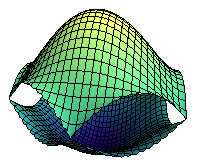
\includegraphics{Figs_TightBinding/bandstructure_3.png}};
	\node at (-3.75,-.5) {$\bm{K}$};
	\node at (-.25,-2)[fill=white, rounded corners]{$\bm{K'}$};
\end{tikzpicture}
	\end{center}
	\caption{\label{fig:TB:Dispersion} The electronic dispersion in the first Brillouin zone calculated with a nearest neighbor tight binding model.  The two energy bands meet at the $\bm{K}$ and $\bm{K'}$ points.}	
\end{figure}

The two points of convergence between the high and low energy bands are referred to as the Dirac points because of the characteristic energy dispersion in their vicinity.
This interesting low energy physics can be best captured by expanding the Hamiltonian in Equation \ref{eq:TB:RealSpace} about these points.
The wave-vectors are approximated as $\vec{k}=\bm{K}+\vec{q}$ and $\vec{k}=\bm{K'}+\vec{q}$ and for small $qa$ the sum in Equation \ref{eq:TB:RealSpace} is approximated as,
\begin{align*}
	\sum_{j} e^{-i \vec{k} \cdot \vec{\Delta}_j}&= \\
	\bm{K:}\ 	&=\sum_{j} e^{-i (\bm{K}+\vec{q}) \cdot \vec{\Delta}_j} \\
				&\simeq \sum_{j} (1-i \vec{q} \cdot \vec{\Delta}_j) e^{-i \bm{K} \cdot \vec{\Delta}_j} \\
				&=-\frac{3}{2} a \left( q_x-i q_y \right) \\
	\bm{K':}\	&\simeq \sum_{j} (1-i \vec{q} \cdot \vec{\Delta}_j) e^{-i \bm{K'} \cdot \vec{\Delta}_j} \\
				&=-\frac{3}{2} a \left(-q_x-i q_y \right) . \\
\end{align*}
These values are independent of which of the three identical $\bm{K}$ or $\bm{K'}$ points are expanded about.
The low energy Hamiltonian is thus,
\begin{align*}
	\bm{K:} \ H&\simeq\frac{3}{2} a t_0 \sum_{\vec q} 
		\left( \begin{array}{cc} a^{\dagger}_{\vec{q}} & b^{\dagger}_{\vec{q}} \end{array} \right)
		\left( \begin{array}{cc}
			0              & q_x - i q_y\\
			q_x+i q_y      & 0                                                 \end{array} \right)
		\left( \begin{array}{c } a_{\vec{q}}           \\ b_{\vec{q}}          \end{array} \right) \\
	  &=\frac{3}{2} a t_0 \sum_{\vec q}
		\left( \begin{array}{cc} a^{\dagger}_{\vec{q}} & b^{\dagger}_{\vec{q}} \end{array} \right)
		\vec{q} \cdot \vec{\sigma}
		\left( \begin{array}{c } a_{\vec{q}}           \\ b_{\vec{q}}          \end{array} \right) \\
	\bm{K':} \ H& \simeq \frac{3}{2} a t_0 \sum_{\vec q} 
		\left( \begin{array}{cc} b^{\dagger}_{\vec{q}} & a^{\dagger}_{\vec{q}} \end{array} \right)
		\left( \begin{array}{cc}
			0              & -q_x + i q_y\\
			-q_x-i q_y     & 0                                                 \end{array} \right)
		\left( \begin{array}{c } b_{\vec{q}}           \\ a_{\vec{q}}          \end{array} \right) \\
	  &=\frac{3}{2} a t_0 \sum_{\vec q}
		\left( \begin{array}{cc} b^{\dagger}_{\vec{q}} & a^{\dagger}_{\vec{q}} \end{array} \right)
		(-1)\vec{q} \cdot \vec{\sigma}
		\left( \begin{array}{c } b_{\vec{q}}           \\ a_{\vec{q}}          \end{array} \right), \\
\end{align*}
or in the combined form:
\begin{align}
	H&=\hbar v_f \sum_{\vec q, \vec{q}}
		\left( \begin{array}{cccc} b^{\dagger}_{\vec{q}} & a^{\dagger}_{\vec{q}} & a^{\dagger}_{\vec{q}} & b^{\dagger}_{\vec{q}}
																							\end{array} \right)
		\left( \begin{array}{cccc}
			0              & q_x - i q_y & 0            & 0 \\
			q_x+i q_y      & 0           & 0            & 0 \\                            
			0              & 0           & 0            & -q_x+i q_y \\
			0              & 0           & -q_x-i q_y & 0			            			\end{array} \right)
		\left( \begin{array}{c } b_{\vec{q}} \\ a_{\vec{q}} \\ a_{\vec{q}} \\ b_{\vec{q}}  \end{array} \right) \nonumber \\
	H&=\sum_{\vec q, \vec{q}}
		\left( \begin{array}{cccc}  a^{\dagger}_{\vec{q}} & b^{\dagger}_{\vec{q}}&  b^{\dagger}_{\vec{q}} & a^{\dagger}_{\vec{q}}
																							\end{array} \right)
		\left( \begin{array}{cc}
			v_f \vec{p} \cdot \vec{\sigma}              & 0\\
			0              & v_f \vec{p} \cdot \vec{\sigma}			   	            			\end{array} \right)
		\left( \begin{array}{c }  a_{\vec{q}} \\ b_{\vec{q}} \\  b_{\vec{q}} \\ a_{\vec{q}} \end{array} \right)
	\label{eq:TB:FullH}
\end{align}
with $\vec{\sigma}= \left( \begin{array}{cc} 0 & 1 \\ 1 & 0 \end{array} \right) \hat{x}+\left( \begin{array}{cc} 0 & -i \\ i & 0 \end{array} \right) \hat{y}$ is the vector of Pauli matrices and $v_f$ is the Fermi velocity given by $\frac{3}{2}\frac{at}{\hbar} \sim .9 \times 10^6 \ m/s$.
To express the Hamiltonian near the $\bm{K'}$ point in terms of Pauli matrices, the order of the raising and lower operators had to be switched.
This subtle difference means that the first component of eigenvectors for electrons the near $\bm{K'}$ corresponds to the amplitude for an electron on the B sub-lattice, not the A sub-lattice.
These approximate Hamiltonians will be central for the discussion of electron physics in manipulated graphene.

The eigenvalues near either $\bm{K}$ or $\bm{K'}$ are easy to solve for using the low energy Hamiltonians.
At both points, the low energy electronic dispersion is identical,
\begin{equation*}
	E=\hbar v_f |\vec{q}| \ .
\end{equation*}
As shown in Figure \ref{fig:TB:Dispersion}, the high and low energy bands meat at points at the Dirac points.
Away from this point, the energy scales linearly with momentum measured from the Dirac point.
Reminiscent of the light cone, this canonical dispersion is characteristic of a massless particle.

From the low energy electronic dispersion the density of electronic states can be directly calculated for the two dimensional system.
After taking account of the two full spin and two fold valley degeneracy, the density of states is
\begin{equation}
	\rho(\epsilon)=\frac{2}{\pi} \left( \frac{\hbar v_f}{L} \right)^2 \epsilon \ ,
\end{equation}
where $L^2$ is the area of the graphene and $\epsilon$ the energy measured from the Dirac points.
This is linear in energy due to the canonical energy dispersion.
The number of states at a given energy is related to the circumference of the Dirac cone at this energy.
Using the density of states the chemical potential can be calculated in standard graphene transport experiments.

Graphene's two dimensional nature makes it simple to continuously modify the chemical potential.
Rather than varying the concentration of dopants as must be done for most three dimensional systems, graphene only requires the application of a back gate voltage.
A standard graphene gated device is shown in Figure \ref{fig:TB:FET}.
Changing the back gate voltage ($V_{BG}$) charges the graphene-backgate capacitor, introducing charges into the system.
In general, the differential increase in the number of charges is $dQ=C(\mu) dV$.
The capacitance is defined as:
\begin{equation}
	C=\frac{d N}{d \mu}
\end{equation}
where $N$ is the number of electrons in the graphene and $\mu$ is the chemical potential.
For intrinsic graphene the capacitance is continuous and the total number of charges is just $N=CV/e$.
The gated graphene device shown in Figure \ref{fig:TB:FET} can be treated as a parallel plate capacitor with a plate separation of 285 nm and the dielectric constant of silicon dioxide.
Matching the integrated density of states to the number of charges in the system relates the applied gate voltage to different measurements of the chemical potential in the system.
Some useful relationships are:
\begin{align*}
	n(cm^{-2})&\sim 7 \times 10^{10} V_{BG} (Volts) \\
	\mu(meV) &\sim 30 \sqrt{V_{BG} (Volts)} \\
	\mu(meV) &\sim 1 \times 10^{-7} \sqrt{n(cm^{-2})}
\end{align*}

\begin{figure}
	\begin{center}
	\newcommand{\FEThw}{4 cm}			% Width--1 cm=1 um
\newcommand{\FETsiot}{.3 cm}		% SiO2 thickness
\newcommand{\FETsit}{.7 cm}			% Si thickness
\newcommand{\FETaut}{0.06 cm}		% Au thickness
\newcommand{\FETauw}{2 cm}			% Separation and width of the gold pad
\begin{tikzpicture}[scale=1,
	sio2/.style={fill=blue!50!white,draw=none},
	si/.style={top color=black!20!white, bottom color=white},
	siedge/.style={draw=black!35!white},
	au/.style={fill=yellow,draw=black!20!yellow,rounded corners=1 pt},
	wire/.style={semithick}]
	
	%The SiO2
	\filldraw[sio2] (-\FEThw,0) rectangle (\FEThw,\FETsiot);

	%The Si
	\shade[si] (-\FEThw,-\FETsit) rectangle (\FEThw,0);
	\draw[siedge] (-\FEThw,0) -- (\FEThw,0);

	%The Gold contacts
	\filldraw[au] (-\FEThw*.9,\FETsiot) rectangle +(\FETauw,\FETaut);
	
	%The Graphene on the top
	\draw[semithick] (-3*\FEThw/4,\FETsiot) -- (3*\FEThw/4,\FETsiot);

	%The wires connecting the gate etc.
	\node (VBG) at (-1.25*\FEThw,0) [circle,draw=black]{$V_{BG}$};
	\draw[wire]  (VBG.north) -- (-1.25*\FEThw,2.5*\FETsiot+2.5*\FETaut) -- (-\FEThw*.9,2.5*\FETsiot+2.5*\FETaut) -- (-\FEThw*.	9,\FETsiot+\FETaut);
	\draw[wire]  (VBG.south) -- (-1.25*\FEThw,-1.25*\FETsit) -- (0,-1.25*\FETsit) -- (0,-.5*\FETsit);

	%Scale bar
	\draw[draw=black,ultra thick,xshift=.75*\FEThw, yshift=-\FETsit*1.25] (-.5 cm,0) -- node[anchor=north] {$1 \ \mu m$}(.5 cm, 0);

\end{tikzpicture}
	\end{center}
	\caption{\label{fig:TB:FET} Side view of a back gated graphene device.  The graphene is on top of 285 nm of thermal oxide grown on heavily doped Si. }	
\end{figure}

\section{Dirac-Weyl electrons}
Graphene's linear electrical dispersion is peculiar.
According to the usual expression for the effective mass of an electron in an electric field, $m^*=\frac{\hbar^2}{\left(\frac{d^2 E}{d k^2}\right)}$, \cite{Kittel2005} the electrons in graphene have infinite mass.
In a classical sense, this is understandable.
The electron's group velocity, $d \omega/d k$ is constant; it can not be changed by applying a force.
Classically, this corresponds to the case of an infinite mass which cannot be accelerated.
An alternative, and more enlightening, interpretation of graphene's properties is as a massless, relativistic, spin 1/2, fermion.
In this scenario the group velocity cannot be changed because the electrons are moving at the systems effective light speed.
Hence, like a photon moving at the speed of light graphene's electrons cannot be accelerated.

In 1984 Semenoff demonstrated that there is an exact correspondence between the low energy Hamiltonian of graphene and the two dimensional Dirac-Weyl Hamiltonian\cite{Semenoff1984} which governs massless, relativistic, spin 1/2, Fermions.
In this section this correspondence will be briefly discussed.

The Hamiltonian of general, relativistic, spin 1/2, fermions is known as the Dirac equation.
It is a matrix equation which is covariant, obeys the relativistic energy expression, and is first order in time.
For the special case of massless particles, the expression is simplified by a wisely chosen representation and is written as
\begin{equation*}
	H=\left( \begin{array}{cc}
			c \vec{p} \cdot \vec{\sigma}              & 0\\
			0              & c \vec{p} \cdot \vec{\sigma}			   	            			\end{array} \right)
\end{equation*}
which, for particles in two spatial dimensions, is identical to Equation \ref{eq:TB:FullH}.
It is clear now that the electrons in graphene behave like relativistic particles in a system where the speed of light is given by the fermi velocity.

As was the case in graphene, the Hamiltonian represents a decoupled system.
In response to this, the wave function is written as the combination of two, two element spinors:
\begin{equation*}
	\psi=\left( \begin{array}{c} \chi_{+} \\ \chi_{-} \end{array} \right)
\end{equation*}
It can be shown that the spinners have well defined and opposite helicities.
Since the energy of these massless particles is given by $\pm p c$, the Hamiltonian can be rewritten in a simpler form known as Weyl's equations,
\begin{align*}
	(1 \mp \vec{\sigma} \cdot \hat{p}) \chi_{+}&=0 \\
	(1 \pm \vec{\sigma} \cdot \hat{p}) \chi_{-}&=0 \ ,
\end{align*}
where $\hat{p}$ is the unit vector in the direction of the momentum.
From this form it is clear that the spinors are eigenvectors of the helicity operator, $\hat{h}=\frac{1}{2} \vec{\sigma} \hat{p}$, with eigenvectors $\hat{h} \chi_+=\pm 1/2$ and $\hat{h} \chi_-=\mp 1/2$.
The $\chi_+$ spinor is said to be right handed; for particles with positive energy the spin and momentum are in the same direction whereas for particles with negative energy they are in the opposite direction.
The $\chi_-$ spinor then is left handed.
Since the helicity operator commutes with the Hamiltonian, helicity is conserved in this system.
Gottfried and Yan provide a more detailed discussion of the Dirac equation and its consequences\cite{Gottfried2003}.

In graphene, the elements of the wavevector have a geometric interpretation.
They correspond to the amplitude that the electron is at the A or B sublattice.
Identifying these components with the relativistic components yields the pseudo spinners: $\psi_+ \equiv \left(\begin{array}{c} \psi_A^{\bm{K}} \\ \psi_B^{\bm{K}} \end{array} \right)$ and $\psi_- \equiv \left(\begin{array}{c} \psi_B^{\bm{K'}} \\ \psi_A^{\bm{K'}} \end{array} \right)$.
It is a subtle point that the spinor for the electrons at the $\bm{K'}$ point is in the opposite order than the $\bm{K}$ point.
Thus, the pseudo spin in this system refers to the sublattice.
Further, the wavefunction for electrons at the $\bm{K}$ point are right handed and the electrons at the $\bm{K'}$ are left handed.

Since graphene's Hamiltonian is identical to that of massless, relativistic, spin 1/2 Fermions, the electrons should exhibit the same odd properties that have been predicted by high energy physicists.
These unique properties include the Klein paradox \cite{Young2009}, Zitterbewegung \cite{CastroNeto2009}, and the anomalous quantum Hall effect \cite{Novoselov2005a,Zhang2005}.
	\chapter{Strain-induced vector potentials: Lattice-corrections and engineered pseudo magnetic fields\label{chap:PVP}}

At the intersection of graphene's outstanding mechanical and electrical properties lies a peculiar and provocative coupling.
Certain strain distributions in graphene can trick the electrons into acting as if they were in a magnetic field.
This comes about because strain shifts the crystal momentum of the Dirac points much like the the canonical momentum is shifted in the presence of a magnetic field.
This exotic coupling is made more appealing by the two dimensional elastic nature of graphene.
Not only does the coupling exist in theory, but the material also allows the physical realization of it.

A dazzling glimpse of the feasibility and potential of strain-engineered graphene\cite{Pereira2009a,Guinea2009} has recently emerged with experiments reporting that certain strain profiles can induce Landau quantization and effective pseudomagnetic fields in excess of 300 T\cite{Levy2010,Yan2012,Yeh2011}.
Such physics strongly encourages the prospect of harnessing this unconventional interplay between graphene's unique electronic and impressive mechanical properties to control electronic transport in graphene devices\cite{Pereira2009a,Fogler2008}.

This chapter starts by discussing the theory of the strain-induced vector potentials with an emphasis on the lattice-corrections first introduced by Kitt et al\cite{Kitt2012,Kitt2013}.
This is followed by an examination of the importance of these lattice-corrections in different physical scenarios.
Finally, methods of strain engineering graphene devices are examined with an emphasis on the over pressured hour glass shaped microchamber.
This device cleverly takes advantage of plasmonics to enhance signals from higher pseudo magnetic field regions.

\section{Lattice-corrected strain induced vector potentials}

By distorting the graphene lattice, strain causes the following\cite{Pereira2009}:
(i) for any amount of strain, the Dirac points are displaced from the corners of the unstrained BZ and, furthermore, do not necessarily sit at the corners of the strained BZ;
(ii) the gapless and conical nature of the energy dispersion remains robust, except when the deformation is so strong that the two inequivalent Dirac points merge in a Lifshitz transition (but that probably requires strains of the order 20\%, where the tight-binding description is not reliable anymore);
(iii) at any finite density the Fermi line is deformed from the isotropic circle to an elliptical shape, and two Fermi velocities can be defined along the principal directions\cite{Pereira2009,Pereira2010c,Choi2010}.
All these modifications are significant and happen concurrently. 
Hence a complete description of the electronic and transport properties of strained graphene requires their combined consideration.
For example, the local shift of the Dirac point (i) can hinder or completely suppress electronic propagation across regions of different strain states\cite{Pereira2009a,Fogler2008}.
The anisotropy of the Fermi surface (iii) has direct bearing in measurable quantities such as the anisotropy in electrical resistivity\cite{Kim2009}, optical absorption\cite{Pereira2010c,Pellegrino2010}, and the Raman signature of the 2D peak\cite{Huang2010,Mohr2010a,Frank2011,Yoon2011}.

From the theoretical as well as technical point of view, the effects of strain are frequently considered independently, and one usually isolates the dominant effect for the physical observable of interest.
Referring to the same examples above, the strain-induced corrections to optical absorption arising from inter-band transitions are insensitive to the absolute position of the Dirac point in the BZ, but strongly depend on the velocity anisotropy\cite{Pereira2010c,Pellegrino2010}.
Likewise, the dominant effect across a strain barrier will be the relative position of the Fermi surfaces in the two regions (since this essentially determines the phase space available for transmission), and in a first approach the anisotropy is usually neglected\cite{Fogler2008,Pereira2009a}, since the full description would obfuscate the presentation of the problem.

When the strain-induced shift of the Dirac points (i) is considered independently of (ii) and (iii), it can be thought of as a pseudo vector potential\cite{Sasaki2005,Ando2006,Manes2007,CastroNeto2009,Vozmediano2010}.
This can be done because of the peculiar form of the strain corrections to the electronic dispersion in graphene.
Electrons in strained graphene are still governed by a Dirac equation, but one in which the strain modifications can be completely absorbed in the replacement $\bm{p} \to \bm{p}-e\bm{A}$ where $\bm{A}$ is the pseudo vector potential.
This matches the conventional minimal coupling scenario, which means that the electrons respond to the deformation-induced perturbation as they would to an external magnetic field.  
The pseudo vector potential is related to the shift in the Dirac point, $\Delta \bm{k}_D$, through $\Delta \bm{k}_D=-\frac{e}{\hbar} \bm{A}$.
This analogy between strain-induced and real magnetic fields means, for example, that the electronic energy levels can be quantized with a relativistic Landau spectrum just as if they were under a real magnetic field given by $\bm{B}=\bm{\nabla}\times\bm{A}$ (as long as this pseudomagnetic field is relatively constant on scales not smaller than the corresponding magnetic length)\cite{CastroNeto2009}.

An omission in earlier work in the context of these pseudo vector potentials is the explicit consideration of the deformation of the lattice when computing the position of the new Dirac points.
Here we include this effect, and show its importance in describing the absolute position of the Dirac points, and the resulting pseudo vector potentials.
This yields new leading order terms in the strain-induced pseudo vector potential which are different at the three inequivalent Dirac points.
Specifically, we shall be interested below only in how strain affects the position of the Dirac point in reciprocal space.
We also restrict the discussion to planar deformations, and hence ignore effects that might arise in the presence of curvature \cite{CastroNeto2009,Vozmediano2010}.
We will detail the derivation of these terms and then demonstrate their importance in describing the shift of the Dirac point in graphene.

The key elements underlying strain induced vector potentials is captured by generalizing the tight binding Hamiltonian discussed in Chapter \ref{chap:TB} to the geometry of the strained graphene.
Figure \ref{fig:PVP:lattice} illustrates the change in lattice geometry due to strain.
For reference the unstrained graphene geometry discussed in Chapter \ref{chap:TB} is included in the first row of Figure \ref{fig:PVP:lattice} with the real space lattice in (a) and the first Brillouin zone in (b).
Figure \ref{fig:PVP:lattice}(c) shows the distortion of the lattice for 20\% uniaxial strain in the armchair direction and Figure \ref{fig:PVP:lattice}(d) shows the corresponding distortion of the Brillouin zone.
The magnitude of strain is not necessary; all of the effects discussed here are linear in strain and thus persist at much smaller strains.
Such a large strain is chosen here to better illustrate strains effect on the geometry.

\begin{figure}
  % Geometry taken directly from my lectures notes on tight binding in graphene
\newcommand{\alat}{1 cm}
\newcommand{\sqth}{1.73205080757}
\newcommand{\Klen}{2 cm}
\begin{tikzpicture}[>=stealth,scale=.8,
		nnarrow/.style={color=black,very thick, ->},					% Nearest neighbor vectors
		nnarrows/.style={color=red,very thick, dashed, ->},				% Strained nearest neighbor vectors		
		lvarrow/.style={color=black, ->},								% lattice vector unstrained
		lvarrows/.style={color=red, dashed, ->},						% Lattice vector strained
		BZ/.style={color=black,fill=black,very thick},					% Unstrained BZ lines
		BZs/.style={color=red,fill=red,dashed, very thick},				% Strained BZ lines
		circ2/.style={radius=1.5pt},									% Dots at K points on BZ
		A/.style={circle,draw=black!50,fill=black!20,
			thick,minimum size=2 mm,inner sep=0pt}, 					% A sublattice dots (unstrained)
		As/.style={circle,draw=red!50,fill=red!20,
			thick,minimum size=2 mm,inner sep=0pt}, 					% A sublattice dots (strained)
		B/.style={circle,draw=black!70,fill=black!40,
			thick,minimum size=2mm,inner sep=0pt},						% B sublattice dots (strained)
		Bs/.style={circle,draw=red!70,fill=red!40,
			thick,minimum size=2mm,inner sep=0pt}]						% B sublattice dots (unstrained)					

	% Graphene lattice, sublattices different colors, nearest neighbor vectors and lattice vectors
	\begin{scope}[xshift=-3.5 cm,yshift=1.5 cm]				% Lattice vector arrows

		%This scope is clipped to limit the drawn lattice to a square
		\clip (-2.75cm,-2cm) rectangle(2.75cm,2.75cm);
		% \draw (-2.75cm,-2cm) rectangle(2.75cm,2.75cm);

		% Draw the unstrained lattice
		\foreach \ip in {-1,0,...,1}
			\foreach \im in {-1,0,...,1}
			{
			\node at (\ip*\sqth*\alat/2-\im*\sqth*\alat/2, \ip*\alat*3/2+\im*\alat*3/2      ) [A] {};
			\node at (\ip*\sqth*\alat/2-\im*\sqth*\alat/2, \ip*\alat*3/2+\im*\alat*3/2-\alat) [B] {};
			}

		% Draw the nearest neighbor vectors
		\draw[nnarrow] (0,0) -- +(270:\alat) node[anchor=north     ]{$\vec{\delta}_1$};
		\draw[nnarrow] (0,0) -- +( 30:\alat) node[anchor=north west]{$\vec{\delta}_2$};
		\draw[nnarrow] (0,0) -- +(150:\alat) node[anchor=north east]{$\vec{\delta}_3$};
		
		% Draw the lattice vectors
		\draw[lvarrow] (0,-\alat/2) -- +( 60:\sqth*\alat)node[circle,anchor=south west]{$\vec{a}_+$};
		\draw[lvarrow] (0,-\alat/2) -- +(120:\sqth*\alat)node[circle,anchor=south east]{$\vec{a}_-$};
	\end{scope}

	% Reciprocal space BZ and high symmetry points
	\begin{scope}[xshift=3.5cm,yshift=1.75 cm,scale=.8]

		% Draw the BZ
		\draw[BZ]
			(  0:\Klen) circle[circ2] node[anchor=west      ]{$\bm{K} $} --
			( 60:\Klen) circle[circ2] node[anchor=south west]{$\bm{K'}$} --
			(120:\Klen) circle[circ2] node[anchor=south east]{$\bm{K }$} -- 
			(180:\Klen) circle[circ2] node[anchor=east      ]{$\bm{K'}$} -- 
			(240:\Klen) circle[circ2] node[anchor=north east]{$\bm{K }$} -- 
			(300:\Klen) circle[circ2] node[anchor=north west]{$\bm{K'}$} -- 
			(  0:\Klen);

		% Label the high symmetry points
		\draw[BZ] (0,0) circle[circ2] node[anchor=west]{$\Gamma$};
	\end{scope}

	% Strained lattice
	\begin{scope}[xshift=-3.5 cm,yshift=-4 cm]
		%This scope is clipped to limit the drawn lattice to a square
		\clip (-2.75cm,-2cm) rectangle(2.75cm,2.75cm);
		% \draw (-2.75cm,-2cm) rectangle(2.75cm,2.75cm);

		% Draw the unstrained lattice
		\foreach \ip in {-1,0,...,1}
			\foreach \im in {-1,0,...,1}
			{
			\node at (\ip*\sqth*\alat/2-\im*\sqth*\alat/2, \ip*\alat*3/2+\im*\alat*3/2      ) [A] {};
			\node at (\ip*\sqth*\alat/2-\im*\sqth*\alat/2, \ip*\alat*3/2+\im*\alat*3/2-\alat) [B] {};
			}

		% Draw the strained lattice
		\foreach \ip in {-1,0,...,1}
			\foreach \im in {-1,0,...,1}
			{
			\node at (\ip*.837*\alat-\im*.837*\alat, \ip*\alat*1.8+\im*\alat*1.8          ) [As] {};
			\node at (\ip*.837*\alat-\im*.837*\alat, \ip*\alat*1.8+\im*\alat*1.8-1.2*\alat) [Bs] {};
			}

		% Draw the unstrained nearest neighbor vectors
		\draw[nnarrow] (0,0) -- +(270:\alat);
		\draw[nnarrow] (0,0) -- +(30 :\alat);
		\draw[nnarrow] (0,0) -- +(150:\alat);

		% Draw the strained nearest neighbor vectors
		\draw[nnarrows] (0,0) -- +(    0*\alat,-1.2*\alat);
		\draw[nnarrows] (0,0) -- +( .837*\alat, .60*\alat);
		\draw[nnarrows] (0,0) -- +(-.837*\alat, .60*\alat);

		% Draw the unstrained lattice vectors
		\draw[lvarrow] (0,-\alat/2) -- +( 60:\sqth*\alat);
		\draw[lvarrow] (0,-\alat/2) -- +(120:\sqth*\alat);

		% Draw the strained lattice vectors
		\draw[lvarrows] (0,-\alat/2) -- +( .837*\alat,1.8*\alat);
		\draw[lvarrows] (0,-\alat/2) -- +(-.837*\alat,1.8*\alat); 
	\end{scope}

	% Strained BZ
	\begin{scope}[xshift=3.5 cm,yshift=-3.75 cm,scale=.8]
		% Draw the unstrained BZ
		\draw[color=black,very thick]
			(  0:\Klen)  --
			( 60:\Klen)  --
			(120:\Klen)  -- 
			(180:\Klen)  -- 
			(240:\Klen)  -- 
			(300:\Klen)  -- 
			(  0:\Klen);

		% Draw the strained 
		\draw[BZs]
			( .917*\Klen, .000*\Klen) circle[circ2] node[anchor=west      ]{$\bm{K_1} $} --
			( .633*\Klen, .693*\Klen) circle[circ2] node[anchor=south west]{$\bm{K_3'}$} --
			(-.633*\Klen, .693*\Klen) circle[circ2] node[anchor=south east]{$\bm{K_2}$} -- 
			(-.917*\Klen, .000*\Klen) circle[circ2] node[anchor=east      ]{$\bm{K_1'}$} -- 
			(-.633*\Klen,-.693*\Klen) circle[circ2] node[anchor=north east]{$\bm{K_3}$} -- 
			( .633*\Klen,-.693*\Klen) circle[circ2] node[anchor=north west]{$\bm{K_2'}$} -- 
			( .917*\Klen, .000*\Klen);

		% Label the high symmetry points
		\draw[BZs] (0,0) circle[circ2] node[anchor=west]{$\Gamma$};
	\end{scope}


	% (a) (b) (c) and (d) labels
	\node at (-7cm,4cm)   {\textbf{(a)}};
	\node at ( 1cm,4cm)   {\textbf{(b)}};
	\node at (-7cm,-1.5cm){\textbf{(c)}};
	\node at ( 1cm,-1.5cm){\textbf{(d)}};

	% Strain labels on the right side
	\node at (-10cm, 1.25 cm) {$\bm{\nabla u}=\left(\begin{array}{cc} 0 & 0 \\ 0 & 0 \end{array}\right)$};
	\node at (-10cm,-4.25 cm) {$\bm{\nabla u}=\left(\begin{array}{cc} -\nu \epsilon & 0 \\ 0 & \epsilon \end{array}\right)$};
\end{tikzpicture}
  \caption{\label{fig:PVP:lattice} (a) Unstrained graphene's real space lattice with labeled nearest neighbor vectors ($\vec{\delta_i}$), labeled lattice vectors, $\vec{a}_+$ and  $\vec{a}_-$, and with light and dark dots representing the A and B sub-lattices, respectively. (b) The Brillouin zone of unstrained graphene with labeled high symmetry points. (c) The change in the real space lattice after the application 20 \% uniaxial strain in the $\hat{y}$ direction.  Red dots represent the position of the strained atoms and red dashed lines are the strained nearest neighbor and lattice vectors which are referred to as $\vec{\delta}_i'$ and $\vec{a}_i'$ respectively.  (d) The unstrained (black, solid) and strained (red, dashed) Brillouin zone, also for 20 \% armchair uniaxial strain, with the now inequivelent inequivalent Dirac points labeled.  $\bm{\nabla u}$ is the displacement gradient tensor detailing the distortion for each row.}
\end{figure}

Figure \ref{fig:PVP:lattice}(c) provides a qualitative geometric picture for how strain alters the unstrained nearest neighbor tight binding approach discussed in Chapter \ref{chap:TB}.
The method of calculating the distortion of the real and reciprocal space lattices is discussed in detail later in this chapter.
The noticeable geometric distortion of both the nearest neighbor vectors and the lattice vectors corresponds to two distinct changes in the tight binding prescription.
The anisotropic alteration of the nearest neighbor vectors modifies the distances between atoms introducing a bond-dependent nearest neighbor hoping amplitude into the unstrained real space Hamiltonian (Equation \ref{eq:TB:baseham}) \cite{Hasegawa2006}
\begin{equation}
  H=-\sum_{<i,j>} \left( t_{i,j} a_i^{\dagger} b_j + t_{j,i} b_j^{\dagger} a_i \right) \ ,
  \label{eq:PVP:RealSpace}
\end{equation}
where $t_{i,j}$ is the bond specific hoping energy.
The second, and oft neglected alteration is a result of the distortion of the lattice vectors.
Their alteration necessitates a change in the phase factors in the Fourier expansion of the creation and annihilation operators in Equation \ref{eq:TB:FT},
\begin{align}
  a_i^{\dagger}&=\frac{1}{\sqrt{N}}\sum_{\vec{k} } e^{ i \vec{k}  \cdot \vec{R}_i'} a_{\vec{k} }^{\dagger} \nonumber \\
  b_j          &=\frac{1}{\sqrt{N}}\sum_{\vec{k}'} e^{-i \vec{k}' \cdot \vec{R}_j'} b_{\vec{k}'} \ . \label{eq:PVP:FT} 
\end{align}
where $\vec{R}_i'$ and $\vec{R}_j'$ are the positions of the atoms in the strained A and B sub-lattices respectively.
They are not controllable independently in an actual physical system; the latter is a consequence of the former.
Past works have ignored the modification of the relative positions of the atoms.

A necessary and non-trivial first step toward including these modifications in the tight binding description is determining how the lattice vectors and nearest neighbor vectors are altered by strain.
This directly determines how the Fourier transforms in Equation \ref{eq:TB:FT} should be altered and is also useful for determining how the hopings in Equation \ref{eq:TB:baseham} are altered.
In general the strain is not uniform and the distortion of these vectors has a spatial dependence.
In continuum mechanics the elastic deformation field, $\vec{u}(\vec{r})$, which detail the shifts in position generated by  deformation is calculated based on macroscopic quantities.
Here we follow the Cauchy-Born rule which projects these macroscopic quantities onto the atomic lattice.
In this approximation, the position of the $i$-th atom in the deformed configuration, $\vec{R}'_i$, is given with reference to the undeformed one, $\vec{R}_i$, in terms of the deformation field
\begin{equation*}
  \vec{R}'_{i}=\vec{R}_{i}+\vec{u}(\vec{R_i}) \ .
\end{equation*}
Although it is feasible that at the atomic scale the A and B sublattices behave differently yet still yield the same macroscopic response, the Cauchy-Born rule provides a simple and reasonable starting point for the discussion of strain effects.
The strained lattice vector at the $i$-th lattice site, $\vec{a}'_{i,\pm}$, is then given approximately by
\begin{align}
  \vec{a}'_{i,\pm}(\vec{r})&=\vec{R}'_j-\vec{R}'_i \nonumber\\
                              &=(\vec{R}_j-\vec{R}_i)+\vec{u}(\vec{R_j})-\vec{u}(\vec{R_i}) \nonumber \\
                              &\simeq\vec{a}_{i,\pm}+(\vec{a}_{i,\pm} \cdot \vec{\nabla}) \vec{u}(\vec{R}_i) \nonumber \\
                              &=\left(\bm{1}+\bm{\nabla u}(\vec{R_i}) \right)\cdot \vec{a}_{i,\pm} \label{eq:PVP:StrainVectors} \ ,
\end{align}
where $\bm{1}$ is the two dimensional identity matrix and the dyadic product $\bm{\nabla u}(\vec{R_i})$ is the Jacobian of the displacement field known as the displacement gradient tensor
\begin{align*}
  [\bm{\nabla u}]_{ij} = u_{i,j} &= \frac{u_{i,j}+u_{j,i}}{2} + \frac{u_{i,j}-u_{j,i}}{2} \\
                       &\equiv \tilde{\epsilon}_{ij} + \tilde{\omega}_{ij} \\
    \rightarrow \quad \bm{\nabla u} &= \tilde{\bm{\epsilon}} + \tilde{\bm{\omega}}
\end{align*}
where $\tilde{\bm{\omega}}$ is the rotation tensor and $\tilde{\bm{\epsilon}}$ is the \emph{linear} strain tensor which is only one part of the full (Lagrange) strain tensor given by $\bm{\epsilon} = \tfrac{1}{2}(\bm{\nabla u} + \bm{\nabla u}^\top+\bm{\nabla u}^\top\bm{\nabla u}) = \tilde{\bm{\epsilon}} + \tfrac{1}{2}(\bm{\nabla u}^\top\bm{\nabla u})$.
It is important to stress that the often used approximating $\vec{a}'_{i,\pm}(\bm{r})\simeq (\bm{1}+\tilde{\bm{\epsilon}})\cdot \vec{a}'_{i,\pm}$ is only valid if the deformation does not involve local rotation ($\tilde{\bm{\omega}}=0$).
To simplify the notation, the position dependence has been left off of $\bm{\nabla u}$.
Similarly, the strain modified nearest neighbor vectors are $\vec{\delta}'_{i,j}(\vec{r})=(\bm{1}+\bm{\nabla u}) \cdot \vec{\delta}_{j}(\vec{r})$ \cite{Kitt2013} where $i$ keeps track of the spatial dependence by indicating the unit cell and $j \in {1,2,3}$ indicates which of the three nearest neighbor vectors is being referred to.

The distortion of the nearest neighbor vectors causes a bond specific alteration of the hoping energy.
By comparing a tight binding treatment of strained graphene to density functional calculations of the same system, Ribeiro and coworkers showed that the dependence of the hoping energy on the distance between carbon atoms can be parameterized as:
\begin{equation*}
  t(|\vec{\delta}_{i,j}|)=t_0 \exp[-\beta (|\vec{\delta}_{i,j}|/a-1)]
\end{equation*}
with $\beta\approx 3$\cite{Pereira2009,Ribeiro2009,CastroNeto2009}.
An exponential decay is chosen because it correctly predicts both the nearest neighbor and next nearest neighbor hoping energies.
The fact that, the hoping energy is mostly insensitive to the bond angle, greatly simplifies the physics.
Having already established the form for the strained nearest neighbor vectors, their length can be easily computed:
\begin{align*}
  |\delta'_{i,j}|^2&=\left(\vec{\delta}_{j}^{\intercal}+\vec{\delta}_{j}^{\intercal} \ \bf{\nabla u}^{\intercal} \right) \cdot
    \left(\vec{\delta}_{j}+\bf{\nabla u} \ \vec{\delta}_{j} \right) \\
    &=\vec{\delta}_{j}^{\intercal} \vec{\delta}_{j}+
      \vec{\delta}_{j}^{\intercal} \left(\bf{\nabla u}+\bf{\nabla u}^{\intercal} \right) \vec{\delta}_{j}+
      \mathcal{O}(\bf{\nabla u}^2) \\
  \rightarrow |\delta'_{i,j}|&\simeq a+\frac{1}{a} \vec{\delta}_{j} \cdot \epsilon \cdot \vec{\delta}_{j}
\end{align*}
for small strains.
As was done for the displacement gradient tensor, the spatial dependence of the strain tensor is dropped from the notation for simplicity.
As expected, the length of these vectors are dependent only on the symmetric part of the displacement gradient tensor-the strain.
To first order, the bond specific nearest neighbor hoping can be written as
\begin{equation*}
  t_{i,j}=t_0+\delta t_{i,j}=t_0-\beta t_0 \frac{1}{a^2} \vec{\delta}_{j} \cdot \epsilon \cdot \vec{\delta}_{j},
\end{equation*}
or
\begin{align}
  \delta t_{i,1}&=-\beta t_0 \epsilon_{yy} \nonumber \\
  \delta t_{i,2}&=-\beta t_0 \left( \frac{3}{4}\epsilon_{xx} +\frac{1}{4} \epsilon_{yy} + \frac{\sqrt{3}}{2} \epsilon_{xy} \right) \nonumber \\
  \delta t_{i,3}&=-\beta t_0 \left( \frac{3}{4}\epsilon_{xx} +\frac{1}{4} \epsilon_{yy} - \frac{\sqrt{3}}{2} \epsilon_{xy} \right)  \label{eq:PVP:dtij}\ .
\end{align}
This fully defines the strain dependences of the modifications in Equations \ref{eq:PVP:RealSpace} and \ref{eq:PVP:FT}.

All the pieces necessary to modify the nearest neighbor tight binding approach from Chapter \ref{chap:TB} are now in place.
The first modification to include the approximated hoping energy in Equation \ref{eq:PVP:RealSpace},
\begin{equation*}
  H=-\sum_{<i,j>} \left( (t_0+\delta t_{i,j})  a_i^{\dagger} b_j + (t_0+\delta t_{j,i}) b_j^{\dagger} a_i \right) \ .
\end{equation*}
In situations such as the deformation of graphene around a sharp scanning tunneling microscopy tip, is not necessarily true that $\delta t_{i,j} = \delta t_{j,i}$.
In these extreme strain situations the continuum approximation can breaks down, the sub-lattice symmetry can be broken, and it is possible that $\delta t_{i,j} \neq \delta t_{j,i}$.
However, for strains that vary slowly with respect to the lattice spacing, the continuum approximation hold and $\delta t_{i,j} \simeq \delta t_{j,i}$ \cite{Sloan2013}.
This assumption will be made throughout.
As a result, the real space Hamiltonian in Equation \ref{eq:PVP:RealSpace} can be approximated to first order in strain,
\begin{equation*}
  H \simeq -\sum_{<i,j>} \left( t_0+\delta t_{i,j} \right)  a_i^{\dagger} b_j + \text{H.C.} \ ,
\end{equation*}
with the strain dependence $\delta t_{i,j}$ given by Equation \ref{eq:PVP:FT}.

Next, using the expansion of the lattice vectors in Equation \ref{eq:PVP:StrainVectors} the creation and annihilation operators in Equation \ref{eq:PVP:FT} can be expanded to first order in the displacement gradient tensor as
\begin{align*}
  a_i^{\dagger}&\simeq \frac{1}{\sqrt{N}}\sum_{\vec{k} } e^{ i \vec{k}  \cdot (\bm{1}+\bm{\nabla u}) \cdot\vec{R}_i}
      a_{\vec{k} }^{\dagger} \nonumber \\
  b_j          &\simeq \frac{1}{\sqrt{N}}\sum_{\vec{k}'} e^{-i \vec{k}' \cdot (\bm{1}+\bm{\nabla u}) \cdot \vec{R}_j}
      b_{\vec{k}'} \ .
\end{align*}

Finally, as was done in the unstrained case in Chapter \ref{chap:TB} the low energy approximation will be applied.
The wave-vectors will again be approximated as $\vec{k}=\bm{K}+\vec{q}$ and $\vec{k}=\bm{K'}+\vec{q}$ for small $qa$.
This introduces the third, and last, small quantity into the Hamiltonian.

Including the altered hoping energies, the deformed lattice vectors, and using the small energy expansion in the Hamiltonian yields,
\begin{align}
  H&\simeq \sum_{<i,j>} \sum_{\vec{q},\vec{q}'} (t_0+\delta t_{i,j})
\end{align}


In reciprocal space, the Hamiltonian, eq.~\ref{eq:PVP:H-TB}, linearized to first order in strain reads:
\begin{equation}
  H \simeq -\sum_{\vec{k},j} \bigl(
  t_0 + \delta t_j - it_0\vec{k}\cdot\epsilon\cdot\vec{\delta}_j
  \bigr) \, e^{-i\vec{k}\cdot\vec{\delta}_j} \,
  a_{\vec{k}}^{\dagger}b_{\vec{k}} + \text{H.c.}
  \label{eq:H-TB-strain}
\end{equation}
The new term proportional to $\vec{k}\cdot\epsilon\cdot\vec{\delta}_j$ arises from expanding $\exp(-i\vec{k}\cdot\vec{\delta'}_j)$ to linear order in strain. Consequently, it contributes on \emph{equal footing} with $\delta t_j$, which is also of leading order in strain \cite{CastroNeto2009}.

Using the \emph{undeformed} BZ as global reference, and approximating this Hamiltonian near the $\bm{K}$ points, one recovers the form of the unstrained Hamiltonian but with the substitution ($\bm{k} \to \bm{k}-\frac{e}{\hbar} \bm{A}$), where the vector potentials are now given by:
\begin{subequations}\label{pvp-all}
\begin{align}
\vec{A}_{\bm{K_1}}&=-\vec{A}_{\bm{K_1'}}=\frac{\phi_0}{2a} \left( \begin{array}{c} \frac{4}{3\sqrt{3}}\epsilon_{xy}\\ \frac{4}{3 \sqrt{3}} \epsilon_{yy} \end{array} \right) +\vec{A}_p , \label{pvpK1}\\ 
\vec{A}_{\bm{K_2}}&=-\vec{A}_{\bm{K_2'}}=\frac{\phi_0}{2a} \left( \begin{array}{c} \frac{2}{3}\epsilon_{xx}-\frac{2\sqrt{3}}{9} \epsilon_{xy} \\ \frac{2}{3} \epsilon_{xy}-\frac{2 \sqrt{3}}{9} \epsilon_{yy} \end{array} \right)+\vec{A}_p  , \label{pvpK2} \\
\vec{A}_{\bm{K_3}}&=-\vec{A}_{\bm{K_3'}}=\frac{\phi_0}{2a} \left( \begin{array}{c} -\frac{2}{3} \epsilon_{xx}-\frac{2 \sqrt{3}}{9} \epsilon_{xy} \\ -\frac{2}{3} \epsilon_{xy}-\frac{2 \sqrt{3}}{9} \epsilon_{yy} \end{array} \right)+\vec{A}_p  , \label{pvpK3} \\
\intertext{with}
&\vec{A}_p=\frac{\phi_0}{2a} \left( \begin{array}{c} \frac{\beta }{\pi} \epsilon_{xy} \\ \frac{\beta }{2 \pi} (\epsilon_{xx}-\epsilon_{yy}) \end{array} \right),
\label{pvpe}
\end{align}
\end{subequations}
$\phi_0=\frac{h}{e}$, and the various $\bm{K}_i$ points are defined as in Fig.~\ref{fig:PVP:lattice}(d).
The common term $\vec{A}_p$ is proportional to the logarithmic derivative of the hoping, $\beta$, and arises from the hoping perturbations, $\delta t_j$, alone.
It has the expected dependence on the strain tensor components \cite{CastroNeto2009,Vozmediano2010}. 
The herein derived additional terms are the corrections due to lattice deformations.
Since $\beta \approx 3$, the lattice corrections are equally important, not only for being of the same order in strain, but for having similar numerical coefficients.
It is also worth emphasizing that taking explicit consideration of the lattice deformations leads to a vector potential that is different for all the corners of the BZ.
This is of course expected because under an arbitrary deformation the equivalence among the three $\bm{K}$ and $\bm{K'}$ points is lost.
In fact, the expressions above quantify the fact that upon general deformation of the graphene lattice, the Dirac point no longer lies at $\bm{K_i}$, nor at any of the symmetry points of the deformed BZ, a point emphasized early on \cite{Pereira2009}.
The only remaining constraint is time-reversal symmetry, which forces $\vec{A}_{\bm{K_i}} = - \vec{A}_{\bm{K_i^\prime}}$.
Finally, it should be noted that the pseudovector potential depends on the crystallographic orientation relative to the strain and that, unlike a real vector potential, it has no gauge freedom as it is determined by an observable.

\begin{figure*}
\includegraphics{Figs_PVP/figure_2.pdf}
\caption{(Color online) Contours of the band structure of graphene under tensile isotropic strain, shear strain, uniaxial armchair strain, and zig-zag strain (rows), for $\epsilon=1\%$ near the three $\bm{K}$ points (columns). The contours are overlaid with the Brillouin zone of unstrained (solid, black)  and strained (dashed, brown) graphene. Vectors mark the displacement of the Dirac points predicted by the traditional ($\vec{A}_p$, dashed/red arrow) and the corrected ($\vec{A}_{\bm{K}_{\!i}}$, solid/orange arrow) form of the pseudo vector potential (eqs.~\ref{pvp-all}), with the green dots marking the positions of the Dirac points for strained graphene. The red vectors appears as a dot for isotropic strain because the traditional form of the vector potential does not predict a shift in the Dirac points.  Each plot is square with an area of $0.12^2$. \label{fig:PVP:PVPshifts}}
\end{figure*}


\section{Discussion}

All existing calculations consider only the term $\vec{A}_p$ and, as a result do not properly account for the shift in the Dirac points.
Consider, for example, the seemingly trivial case of tensile isotropic strain.
The traditional form of the pseudovector potential, $\vec{A}_p$, predicts that there should be no shift in the Dirac points ($\epsilon_{xx}=\epsilon_{yy}$ and $\epsilon_{xy}=0$ in equation \ref{pvpe}).
However, the BZ shrinks isotropically under tensile isotropic strain, and, by symmetry, the Dirac points should follow the corners of the deformed BZ resulting in a Dirac point dependent shift toward the $\Gamma$ point with respect to the unstrained reference state.
In Fig.~\ref{PVPshifts}, the reciprocal space shifts of the Dirac points predicted by the traditional and herein corrected forms of the pseudovector potential are compared.
The contours are the strained band structure calculated using a nearest neighbor tight binding model which accounts for both the strain induced changes in hoping amplitudes and the lattice deformation\cite{Pereira2009}.
For isotropic tensile strain, the lattice-corrected pseudo vector potential in eqs.~\eqref{pvp-all} properly predicts the displacement of each Dirac point due to strain.
The less trivial cases of uniaxial or shear strain are also shown in Fig.~\ref{PVPshifts}. The differences between the red (traditional) and orange (corrected) arrows make it clear that the lattice corrections are needed to determine the absolute position of the Dirac point in reciprocal space (they can even reverse the sign of $\vec{A}$).

As discussed above, these corrections are immaterial for systems with spatially uniform strain but must be included for systems with non-uniform strain.
For example, if there are regions of isotropic tension embedded in regions of different strain states, the relative shifts \emph{are} important, even though deformations are locally isotropic.
In these cases lattice corrections contribute an extra, Dirac point specific, space dependence which is important when calculating transport across a strain barrier or when considering the spatial distribution of the pseudomagnetic fields: $\vec{B}_{\bm{K_i}} = \nabla \times \vec{A}_{\bm{K_i}}$.

In particular, these corrections are critical when trying to optimize the Landau quantization caused by the strain-induced pseudomagnetic fields.
Ideally one desires the pseudomagnetic field to be nearly constant throughout the system so that the Landau levels are as narrow and well defined as possible.
This imposes a delicate and non-trivial constraint on what deformations are compatible with constant pseudomagnetic fields.
An early suggestion uses the traditional form of the pseudovector potential to conclude that strain profiles with an overall trigonal symmetry tend to generate smooth effective pseudomagnetic fields \cite{Guinea2009}.
To show how the lattice correction can quantitatively and qualitatively affect this conclusion, we simulate a situation where graphene is covering an equilateral triangular pit with a uniformly distributed vertical load.
This geometry was originally proposed by Guinea~\emph{et~al.} as a simple method of generating fairly uniform pseudomagnetic fields \cite{Guinea2009}.
We calculate the strain fields using finite element analysis, and extract the local pseudomagnetic fields from eqs.~\eqref{pvp-all}.
The finite element analysis was performed using Comsol Multiphysics, with a two-dimensional thin plate model including geometric non-linearity.
The edges were fixed and the pressure was applied using a face load.
Graphene's Young's Modulus of 1 TPa and thickness of 3.5 \AA \cite{Lee2008} were used along with the Poisson ratio of graphite of 0.165 \cite{Blakslee1970}.
To make the triangles more realistic we include 2 nm radius fillets on the three corners, which smooth down the sharp boundary corners.
The surface was meshed with triangles with a maximum element size of 1 nm, and strain fields were evaluated in the mid-plane of the plate.

\begin{figure*}
\includegraphics{Figs_PVP/figure_3.pdf}
\caption{\label{triholes}The spatial distribution of the pseudomagnetic fields generated when an equilateral triangle with 50 nm sides, 2 nm radius fillets, and the base oriented 30 degrees counterclockwise from the armchair direction is pressurized to 14 MPa. In (a) the calculation is done using the traditional form of the pseudovector potential, while in (b) it is performed including the corrections derived in this work. Here, the three different colored curves correspond to the pseudomagnetic fields felt by the electrons at the three different $\bm{K}$ points with the magnetic field for the electrons at $\bm{K_1}$ isolated in (c). (Color online)}
\end{figure*}

The effect of the lattice corrections to the extracted pseudomagnetic field are shown in Fig.~\ref{triholes} for an equilateral triangle with 50 nm sides, and under 14 MPa of pressure.
At this pressure the graphene sheet has less than 0.26~\% strain.
The field derived from the traditional form of the pseudovector potential \eqref{pvpe} results in a fairly uniform pseudomagnetic field [Fig.~\ref{triholes}(a)], in agreement with Guinea et al \cite{Guinea2009}.
In contrast, Figs.~\ref{triholes}(b,c) show that the new terms cause the electrons near the three different $\bm{K}_{1,2,3}$ points to experience different pseudomagnetic fields, which vary strongly across the system.
The differences in the pseudomagnetic fields at the different Dirac points may be extremely useful in the context of valleytronics \cite{Rycerz2007}.

\section{Conclusion}

In summary, accounting for explicit lattice deformations in the calculation of the pseudo vector potentials generates new leading order, and $\bm{K}$ point specific terms, that are needed to accurately describe the strain dependent shift of the Dirac points in reciprocal space. These terms are important in situations of non-uniform strain, such as when exploring transmission across strain barriers, or when predicting pseudomagnetic fields arising from particular strain profiles.
In those situations the precise space dependence of the pseudo vector potentials, $\vec{A}_{\bm{K}_i}$, and the understanding that they are different at each of the three inequivalent Dirac points is important.

\setlength{\parindent}{0em}
\setlength{\parskip}{1em}

%__________________________________________________________________________________________________________________


The second conclusion is incorrect because, although the corrections $\vec{A}_\text{latt}$ are finite and, in general, have a position dependence, their rotational is identically zero and, thus, so is their contribution to the pseudomagnetic field. This has been pointed out recently by de Juan \emph{et al.}~\cite{DeJuan2013}. Below we elaborate on that, and on the reason why Fig.~3 apparently shows a non-zero $\vec{B}_{\bm{K}_i}$, when it should have been zero by construction. We trust the detail will benefit the reader.




When the correct expansion for the strained position of the atoms is used, it becomes apparent that the lattice corrections cannot contribute to the pseudomagnetic field. Upon expansion around a corner of the BZ of the undeformed lattice, $\bm{K}$, the lattice corrections to the vector potential can be cast as \cite{DeJuan2013}
%
\begin{equation}
  \vec{A}_\text{latt}=\vec{A}_{\bm{K}}-\vec{A}_p \propto \bm{\nabla} (\bm{K}\cdot\bm{u})
  .
\end{equation}
%
Since the above is a total derivative, it cannot contribute to the pseudomagnetic field because $\nabla\times\nabla \phi \equiv 0$. This can be also verified by direct inspection of Eqs.~(4) of the original paper which remain valid in form if the replacement $\bm{\epsilon } \to \bm{ \nabla u }$ is made.

Having clarified and established the correct expansion of the nearest neighbor vector and the lack of an induced pseudomagnetic field a few comments on the results in the original paper are in order:
%
\begin{enumerate} \renewcommand{\theenumi}{\roman{enumi}}
  \item The lattice corrections are still needed to correctly describe the shift in the positions of the Dirac points due to strain. Thus, when the position of the Dirac points is required in a global frame of reference (e.g. to describe momentum-sensitive electronic tunneling to/from strained graphene from/to another system, probe, or contact), Eqs.~4 should be used with the substitution $\bm{\epsilon } \to \bm{\nabla u}$:
%
	\begin{align*}
	\vec{A}_{\bm{K_1}}&=-\vec{A}_{\bm{K_1'}}=\frac{\phi_0}{2a} \left(
\begin{array}{c} \frac{4}{3\sqrt{3}}\bm{[\nabla u]}_{yx}\\ \frac{4}{3
\sqrt{3}} \bm{[\nabla u]}_{yy} \end{array} \right) +\vec{A}_p , \\ 
	\vec{A}_{\bm{K_2}}&=-\vec{A}_{\bm{K_2'}}=\frac{\phi_0}{2a} \left(
\begin{array}{c} \frac{2}{3}\bm{[\nabla u]}_{xx}-\frac{2\sqrt{3}}{9}
\bm{[\nabla u]}_{yx} \\ \frac{2}{3} \bm{[\nabla u]}_{xy}-\frac{2
\sqrt{3}}{9} \bm{[\nabla u]}_{yy} \end{array} \right)+\vec{A}_p  ,  \\
	\vec{A}_{\bm{K_3}}&=-\vec{A}_{\bm{K_3'}}=\frac{\phi_0}{2a} \left(
\begin{array}{c} -\frac{2}{3} \bm{[\nabla u]}_{xx}-\frac{2
\sqrt{3}}{9} \bm{[\nabla u]}_{yx} \\ -\frac{2}{3} \bm{[\nabla
u]}_{xy}-\frac{2 \sqrt{3}}{9} \bm{[\nabla u]}_{yy} \end{array}
\right)+\vec{A}_p  , \\
	\intertext{with}
	&\vec{A}_p=\frac{\phi_0}{2a} \left( \begin{array}{c} \frac{\beta }{\pi} \epsilon_{xy} \\ \frac{\beta }{2 \pi} (\epsilon_{xx}-\epsilon_{yy}) \end{array} \right).
	\end{align*}
%
  \item Eq.~(3) of the original paper,
\begin{equation*}
  H \simeq -\sum_{\vec{k},j} \bigl(
  t_0 + \delta t_j - it_0\vec{k}\cdot\epsilon\cdot\vec{\delta}_j
  \bigr) \, e^{-i\vec{k}\cdot\vec{\delta}_j} \,
  a_{\vec{k}}^{\dagger}b_{\vec{k}} + \text{H.c.}
  ,
\end{equation*}
is written as $\propto \bm{k}\cdot\bm{\epsilon}\cdot\bm{\delta}_i$, when, rigorously, it should have been $\propto\bm{k}\cdot\bm{\nabla u}\cdot\bm{\delta}_i$.
\end{enumerate}
	\chapter{How graphene slides: Measurement and theory of strain-dependent frictional forces between graphene and $\mathrm{SiO_2}$\label{chap:fri}}

Graphene is an amazing mechanical system with extreme elasticity\cite{Lee2008}, ultrastrong adhesion\cite{Koenig2011}, and impermeability to gases\cite{Bunch2008}.
As a pure two dimensional material, graphene's interactions with its supporting substrate are unique.
Amontons' first law states that macroscopic friction is proportional to the applied load, justified by arguing that increasing the load increases the microscopic contact area between two surfaces\cite{Krim1996}.
Graphene, however, because of its ultrastrong adhesion\cite{Koenig2011} and low bending rigidity requires no load to achieve nearly perfect conformation to the nanoscale topography of its substrate, especially the commonly used $\mathrm{SiO_2}$\cite{Stolyarova2007,Lui2009,Cullen2010}.
Hence, the friction between graphene and $\mathrm{SiO_2}$ might be expected to exhibit an atypical load dependence.
The ability to control the thickness of few layer graphene (FLG) at an atomic scale makes it an excellent model system to study the role of thickness and load on friction, which has not previously been quantified or elucidated in detail.
To date most tribological studies of FLG and graphitic materials have measured the interaction between graphene and a scanning probe tip using frictional force microscopy\cite{Dienwiebel2004,Deng2012,Lee2010,Li2010c,Filleter2009,Filleter2010,Zhang2012a}.
These nanoscale measurements have shown interesting effects such as superlubricity in graphite\cite{Dienwiebel2004}, negative frictional coefficient for chemically modified graphite\cite{Deng2012}, and increasing friction with decreasing FLG thickness\cite{Lee2010,Li2010c,Filleter2009,Filleter2010}.
Both the negative frictional coefficient and the increasing friction with decreasing thickness have been attributed to the puckering of graphene about the scanning probe tip\cite{Lee2010,Li2010c,Deng2012}.

Here, for the first time, we directly measure the intrinsic sliding of graphene over a $\mathrm{SiO_2}$ substrate at the macroscopic device scale and, further, extract both the load and atomic layer dependence of sliding friction, or the substrate's resistance to graphene sliding.
We isolate the graphene-substrate interaction and avoid introducing a scanning probe tip to the system by using variable gas pressure applied to an FLG sealed microchamber as shown in Figure \ref{fig:fri:device}.
The pressure acts as a tunable load, simultaneously pressing the supported graphene into the substrate while forcing the suspended FLG into the microchamber.
\emph{In situ} Raman measurements, which can easily measure FLG extensions of $1 \ nm$ over $1 \ \mu m$, show that an annulus of the supported FLG reproducibly slides toward the center of the microchamber.
By analyzing the strain response with a newly derived extension of the continuum Hencky model, we are able to extract load-dependent sliding frictions for mono-, bi-, and tri-layer graphene.
The layer dependence exhibits a crossover between bilayer and trilayer; the trilayer sliding friction obeys Amontons' first law, whereas the monolayer and bilayer sliding friction uniquely scales with the inverse of the strain in the graphene.
We attribute these interesting results to the interplay between adhesion, in-plane strain and bending rigidity in this two dimensional tribological system.
A firm understanding of graphene's sliding friction is necessary for a variety of exciting graphene devices such as flexible bistable displays\cite{Bonaccorso2010}, graphene electro-mechanical switches\cite{Milaninia2009}, strain engineered devices\cite{Pereira2009a} which take advantage of strain induced vector-potentials and pseudomagnetic fields\cite{CastroNeto2009,Guinea2009,Kitt2012}, and high quality factor graphene mechanical resonators\cite{Kim2009b,Bunch2007,Chen2009,Barton2011}.

\begin{figure}
	\begin{center}
	\newcommand{\topthick}{.3 cm}
\newcommand{\botthick}{8 cm}
\newcommand{\basethick}{2 cm}
\newcommand{\edge}{12 cm}
\newcommand{\radius}{5 cm}
\newcommand{\srad}{.5 cm}
\newcommand{\grup}{0 cm}
\begin{tikzpicture}[scale=.25,sio2/.style={fill=blue!50!white,draw=none},siedge/.style={draw=black!50!white}]

	%Image of a hole (top view)
	\begin{scope}[xshift=0 cm,yshift=10 cm]
		\node at (0,0) {
\includegraphics[scale=1.2,trim=1.25cm .45cm 1.25cm .45cm,clip]{Figs_Friction/SB03-2.jpg}};
	\end{scope}
	
	%The SiO2
	\filldraw[sio2] (-\edge,0) -- (-\radius, 0) -- (-\radius, -\topthick) -- (-\edge, -\topthick);
	\filldraw[sio2] (\edge,0) -- (\radius, 0) -- (\radius, -\topthick) -- (\edge, -\topthick);
	
	%The Si
	\fill[fill=black!20!white]
		(-\edge,-\topthick) -- (-\radius,-\topthick) 
		\foreach \i in {0,...,15}
			{-- (-\radius, -\topthick-\i*\srad) .. controls (-\radius-\srad/4, -\topthick-\srad/4-\i*\srad) and (-\radius-\srad/4, -\topthick-3*\srad/4-\i*\srad) ..
			(-\radius,-\topthick-\srad-\i*\srad) }
		-- (-\radius, -\topthick-\botthick) node[anchor=south west] {$P_0$} -- 
		(\radius, -\topthick-\botthick) 
		\foreach \j in {15,14,...,0}
			{-- (\radius, -\topthick-\srad-\j*\srad) .. controls (\radius+\srad/4, -\topthick-3*\srad/4-\j*\srad) and (\radius+\srad/4, -\topthick-\srad/4-\j*\srad) ..
			(\radius,-\topthick-\j*\srad) }
		 -- (\edge, -\topthick) -- 
		(\edge, -\topthick-\botthick-\basethick) -- (-\edge, -\topthick-\botthick-\basethick) [draw=none]-- cycle ;
	
	\draw[siedge](-\edge,-\topthick) --(-\radius,-\topthick);
	\foreach \i in {1,...,16}
		\draw[yshift=-1*(\i-1)*\srad,siedge] (-\radius, -\topthick) .. controls (-\radius-\srad/4, -\topthick-\srad/4) and (-\radius-\srad/4, -\topthick-3*\srad/4) ..
			(-\radius,-\topthick-\srad);
	\draw[siedge] (-\radius, -\topthick-\botthick) -- (\radius, -\topthick-\botthick);
	\draw[siedge] (\radius, -\topthick) -- (\edge, -\topthick);
	\foreach \i in {1,...,16}
		\draw[yshift=-1*(\i-1)*\srad,siedge] (\radius, -\topthick) .. controls (\radius+\srad/4, -\topthick-\srad/4) and (\radius+\srad/4, -\topthick-3*\srad/4) ..
			(\radius,-\topthick-\srad);
	
	\node at (9,1.5) {$N_2$};
	
	%The Graphene on the top
	\draw[thick] (-\edge,\grup) -- (-\radius,\grup) node[anchor=south west]{$P>P_0$}  parabola bend (0,-.7 cm)  (\radius,\grup) -- (\edge,\grup);
	
	%Scale bar
	\draw[draw=black,ultra thick, xshift=\radius/2+\edge/2-2.5cm, yshift=-\botthick-\topthick-\basethick/2] (0,0) -- node[anchor=south] {$5 \ \mu m$}(5 cm, 0);
	
	%Dashed lines
	\draw[color=black!40!white,dashed] (-\edge,\grup+.5cm) -- (-\edge,\grup+4.5 cm);
	\draw[color=black!40!white,dashed] (\edge,\grup+.5cm) -- (\edge,\grup+4.5 cm);
\end{tikzpicture}
	\end{center}
	\caption{\label{fig:fri:device} Top: An optical image of a trilayer graphene-sealed microchamber. Bottom: Device cross-section schematic showing the microchamber etched $8 \ \mu m$ into the underlying Si substrate and the supported graphene atop the 300 nm of thermal oxide.  Pictured to scale is the largest pressure induced deflection of the graphene achieved in any of the analyzed experiments.}
\end{figure}

\section{Raman G band strain response}
Micro-Raman spectroscopy is a powerful tool to measure strain distributions in graphene.
The Raman G band measures the zone center, in-plane optical phonons that are degenerate at zero strain.
In the absence of shear strain, the G band shifts according to\cite{Huang2009}:
\begin{equation}
	\Delta \omega_G=-\omega_0 \gamma(\epsilon_{r}+\epsilon_{t}) \pm \frac{1}{2} \beta (\epsilon_{r}-\epsilon_{t})
\end{equation}
where $\epsilon_{r}$ and $\epsilon_{t}$ are the strain in the radial and tangential directions,  $\gamma$ is the Gr\"{u}neisen parameter and $\beta$ is the shear deformation potential which details the amount of splitting between the $G^+$ and $G^-$ bands.
Light scattered by the $G^+$ and $G^-$  bands has orthogonal linear polarizations\cite{Huang2009}.
Unless otherwise noted, circularly polarized light is used so that the $G^+$ and $G^-$ bands are measured simultaneously.
Figure \ref{fig:fri:circlelinear} shows that the spectra taken using circular polarized light match the sum of the $G^+$ and $G^-$ bands which were measured using linearly polarized light.

\begin{figure}
	\begin{center}
	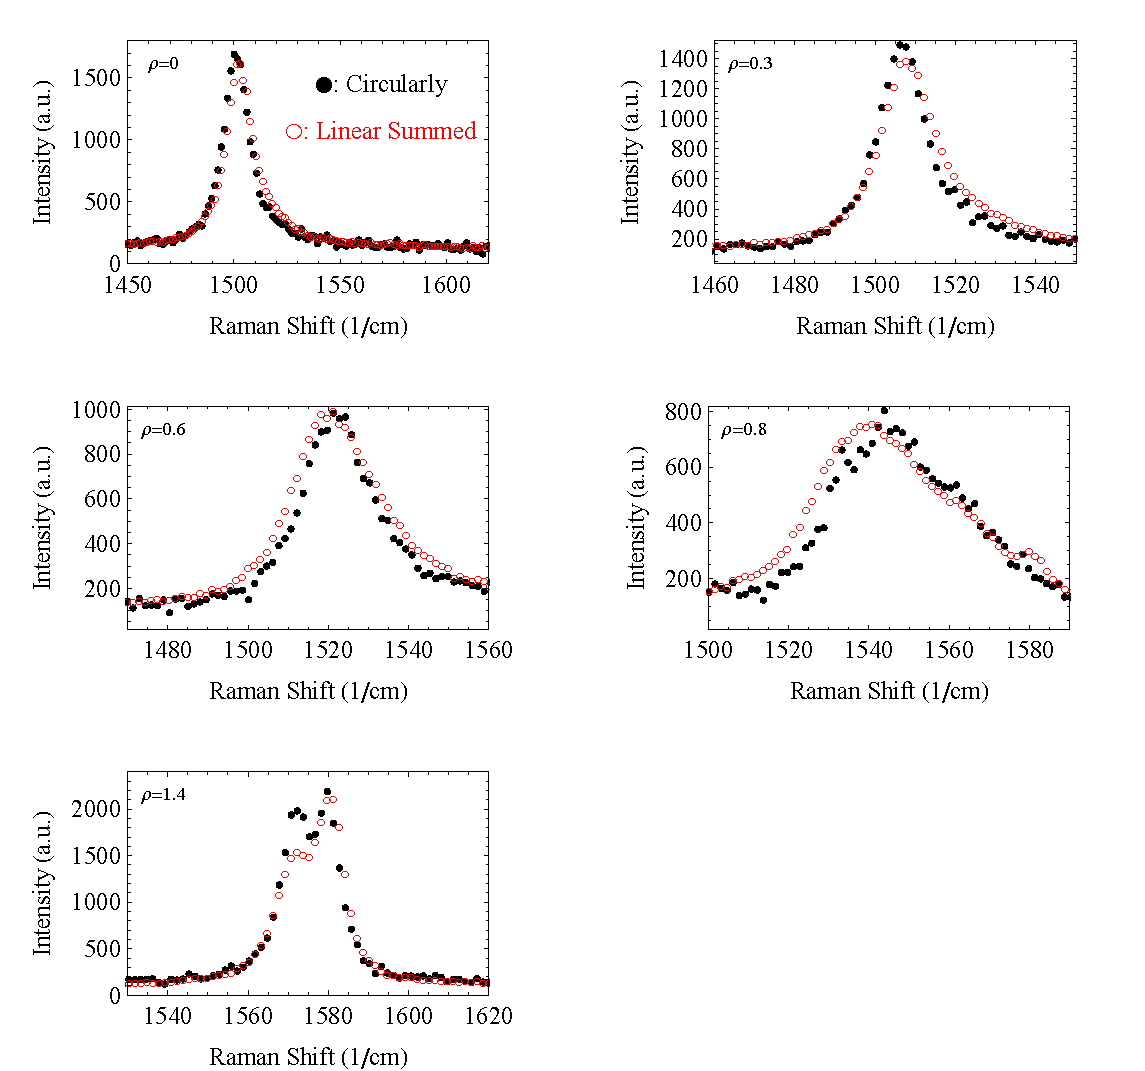
\includegraphics[scale=.75]{Figs_Friction/LinearvsCircular.pdf}
	\end{center}
	\caption{\label{fig:fri:circlelinear}A comparison of Raman spectra measured using circularly and linearly polarized light. Measurements were taken at the labeled positions on a $5 \ \mu m$ radius graphene sealed microchamber with 0.80 MPa of applied absolute pressure. The black dots show the spectrum measured using circularly polarized light while the red dots are the sum of the spectra taken with incident polarization set in the $\hat x$ direction and outgoing polarization analyzed from -90 to 90 degrees in 20 degree steps.  The spectra are scaled to match intensities. Thus, the red dots give the signal from both the $G^+$ and $G^-$ bands measured in the standard linearly polarized way.  The agreement between the red and black dots proves that the measured circularly polarized spectra simply give the sum of the contributions from the $G^+$ and $G^-$ peaks.}
\end{figure}

The local Raman response is measured inside an optically accessible pressure chamber with a focused laser beam while variable pressures up to 0.80 MPa are used to push the FLG into the microchamber.
Raman spectra are excited using the 514 nm line of an argon ion laser and collected using a Renishaw spectrometer with an 1800 lines/mm grating and a 63X, .7 NA, cover slip corrected objective.
The laser power in the pressure chamber was kept below 0.5 mW to avoid sample heating.
The optical access in the pressure chamber is through a 1 mm BK7 window.
The beam waist of the focused laser was measured to be $0.83 \pm .01 \ \mu m$ by scanning a gold pad under the laser as shown in Figure \ref{fig:fri:waist}.

\begin{figure}
	\begin{center}
	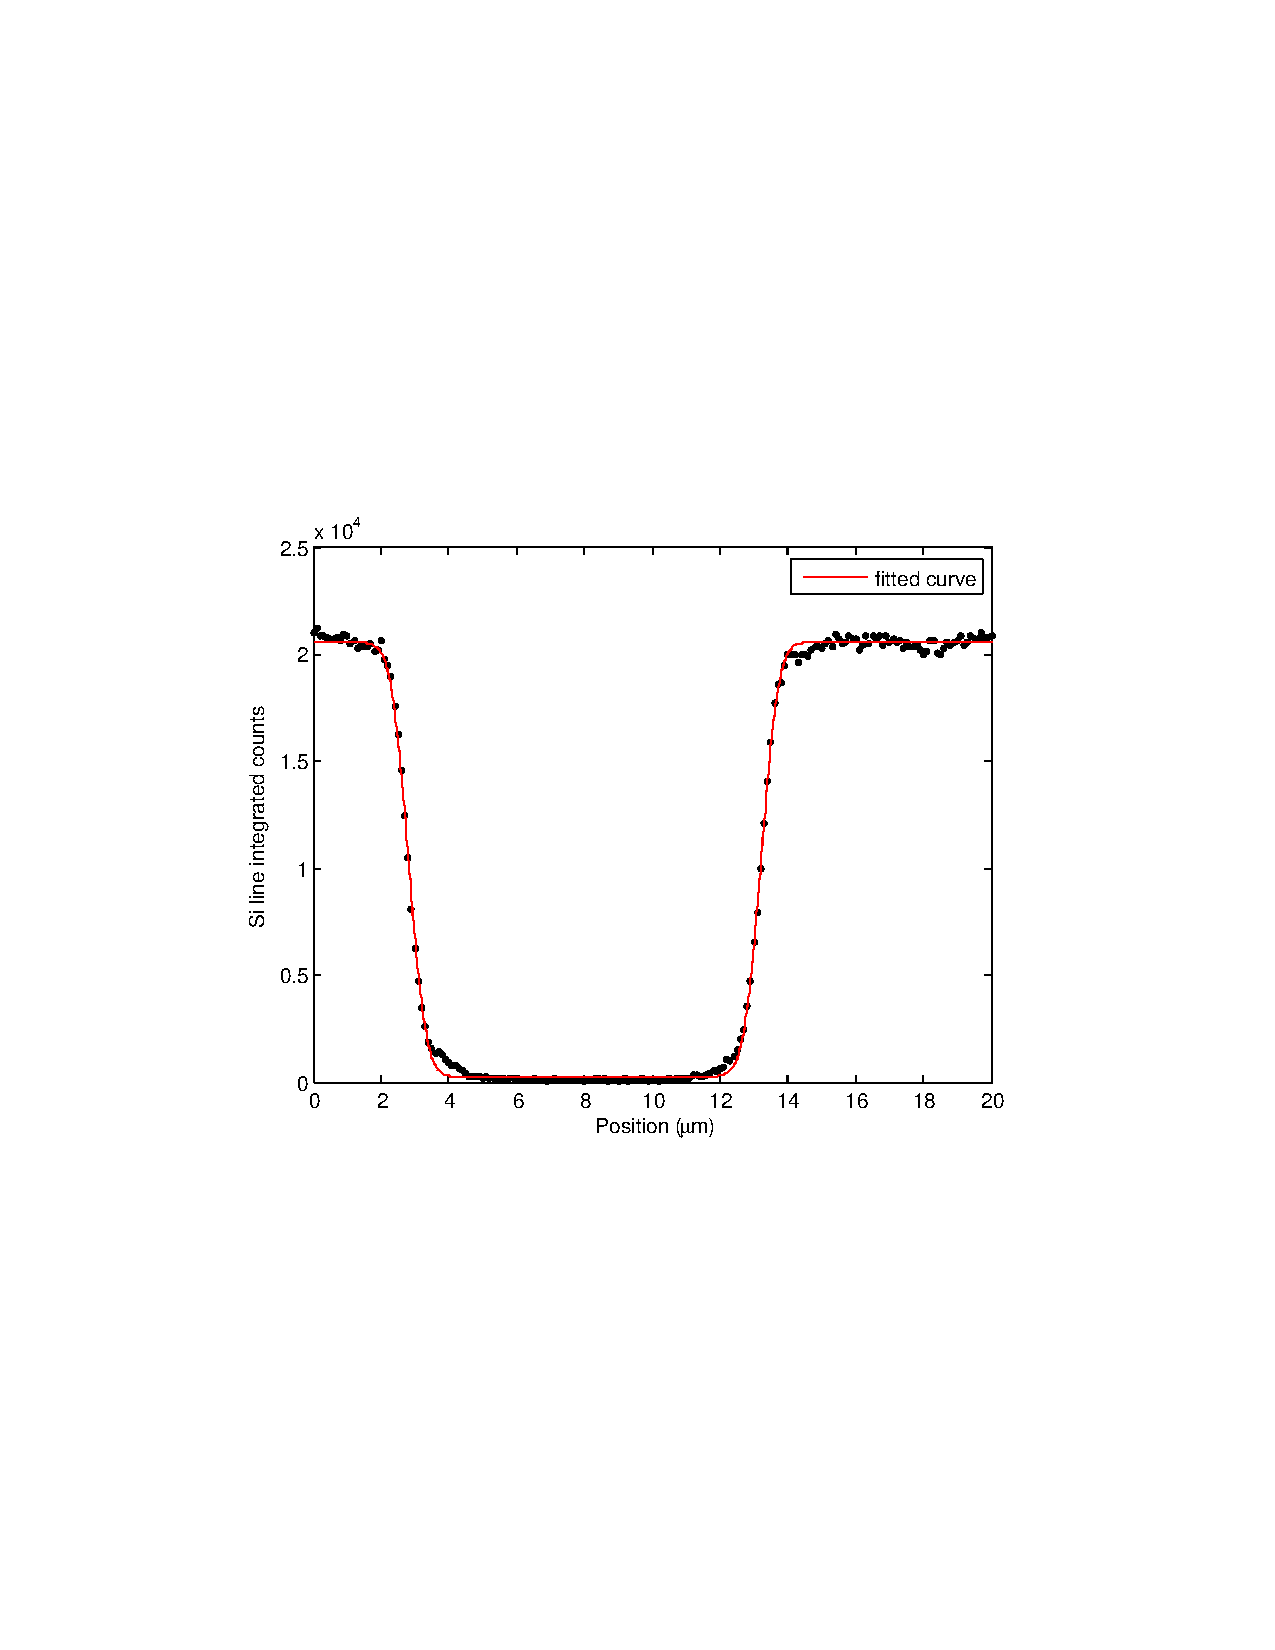
\includegraphics[scale=1]{Figs_Friction/SpotSize.pdf}
	\end{center}
	\caption{\label{fig:fri:waist}Determination of the beam waist of the focused laser in the pressure chamber. A sample with a gold pad was scanned under the focused beam while measuring the Si Raman line intensity. As the sharp edge of the gold pad moves under the laser, the Si line is blocked giving a measure of the beam size. Fitting the signal to an error function gives a beam waist of $0.81 \pm .01 \ \mu m$.}
\end{figure}

\section{Experimental Design}
A cross-section of one of our microchambers sealed with mechanically exfoliated FLG is depicted in Figure \ref{fig:fri:device}.
Microchambers are fabricated using standard optical lithographic methods to define holes ranging from 1 to 5 $\mu m$ in radii,  reactive ion etching to etch through the 300 nm thermal oxide layer, and deep reactive ion etching to etch roughly $8 \ \mu m$ into the underlying silicon layer.
Before the graphene is mechanically exfoliated to seal the microchambers, the substrate is oxygen plasma ashed for 10 minutes at 300 sccm and 500 Watts to ensure the substrate is cleaned of any residues.
The number of graphene layers sealing each device was determined using Raman spectroscopy\cite{Ferrari2006} and optical contrast\cite{Blake2007,Casiraghi2007a}.

The large microchamber depth of $\sim 8 \ \mu m$ is 10 times the largest FLG deflection of $700 \ nm$, allowing us to both ignore changes in internal pressure as the applied pressure is increased, and to measure for longer times because of slower leak-out rates through the silicon substrate.
To eliminate surface residues, the substrate was oxygen plasma ashed before FLG exfoliation.
It is important to note that different surface treatments may yield different sliding frictions providing a new degree of freedom in device engineering. 

Two complementary Raman measurements are performed \emph{in situ} to fully characterize the strain distributions.
First, as the absolute applied pressure is varied between atmospheric pressure (0.10 MPa) and 0.80 MPa, Raman spectra at the center of the microchamber are recorded.
Also, at selected pressures, Raman G band line scans with $ 0.5 \ \mu m$ point spacing are taken across the microchamber.
The former is used to determine the pressure inside of the microchamber while the latter is used to determine the spatial distribution of the strain.
In conjunction with low force ($\approx 1 \ nN$) contact mode atomic force microscopy (AFM), the Raman spectra taken at the center of the microchamber reveal interesting ambient pressure behavior exhibited by the graphene sealed microchambers.

\subsection{Characteristic ambient pressure behavior of FLG sealed microchambers}
The ambient pressure behavior of the measured devices is split roughly evenly between two representative cases.
For half of the devices the pressure inside of the microchamber was greater than ambient, as shown in the left side (a) of Figure \ref{fig:fri:ambient}.
Here, both the AFM and Raman measurements indicate that the pressure inside of the microchamber is greater than ambient.
The topographic image shows the graphene bulging out and the Raman G band response demonstrates that a non-zero gauge pressure is necessary for the G band to reach its greatest, or least strained, value.
By fitting the Raman data with the $p^{2/3}$ form predicted by the standard Hencky model for the strain at the center of the hole (blue dashed line), the internal pressure and unstrained peak position are found.
In the second half of the devices, the pressure inside the microchamber was an atmosphere, as shown on the right side (b) of Figure \ref{fig:fri:ambient}.
The AFM topography shows that the graphene is flat across the aperture indicating the internal pressure matches the ambient pressure.
The graphene is also stuck down to the wall edges for an AFM determined distance of roughly $7 \ nm$.
Other groups have observed similar snap-to-sidewall behavior\cite{Lee2008,Bunch2008}.
Bunch and Dunn noted that the AFM measured distance over which FLG snaps to sidewalls may be overestimated\cite{Bunch2012}, a position supported by our Raman measurements of the strain in these devices.
Additionally, the Raman G band response in these devices shows interesting small strain behavior with increasing pressure which we believe to be a result of graphene peeling off the edge of the walls.
At atmospheric pressure the G band is already red shifted due to pre-strain.
Increasing the gauge pressure to $\sim 0.1$ MPa causes a slower than expected downshift in the G band position.
However, when the gauge pressure is increased beyond $0.1$ MPa, the shift rate converges to the expected trend, $P^{2/3}$, and remains on this trend when the pressure is reduced back to atmospheric pressure.
We believe this is a signature of the FLG unsticking from the walls as pressure is applied and may explain the small Young's Modulus measured by Lee \emph{et al.} using a similar measurement over the a 0.1 MPa pressure range\cite{Lee2012}.

\begin{figure}
	\begin{center}
	\newcommand{\xs}{4.5 cm}
\newcommand{\totscale}{.6}
\newcommand{\afmscale}{.42}
\begin{tikzpicture}[scale=\totscale]
	%SB02-3
	\begin{scope}[xshift=\xs]
		\node at (0,0) {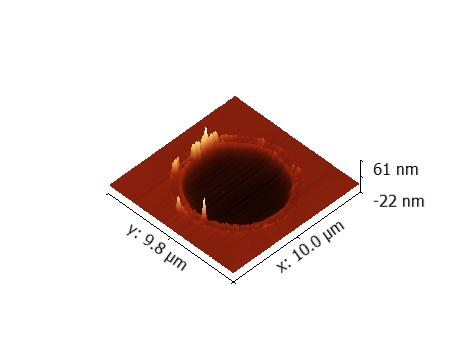
\includegraphics[scale=\afmscale]{Figs_Friction/AFM_SB02-3.jpg}};
		\node at (0,-4.5 cm) {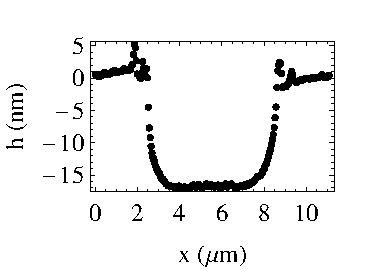
\includegraphics[scale=\totscale]{Figs_Friction/Section_SB02-3.pdf}};
		\node at (0,-10 cm) {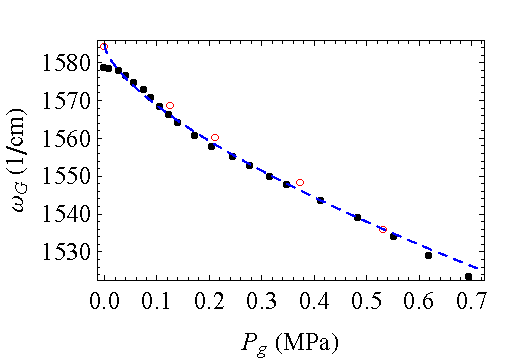
\includegraphics[scale=\totscale]{Figs_Friction/CenterFit_SB02-3.pdf}};
	\end{scope}
	%SB03-2b
	\begin{scope}[xshift=-\xs]
		\node at (0,0) {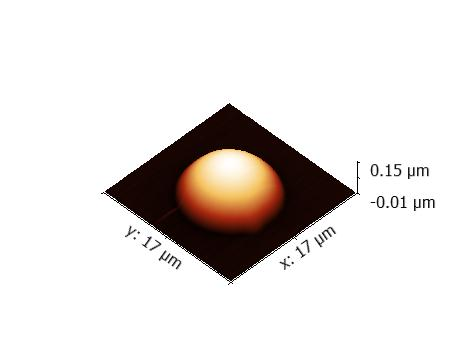
\includegraphics[scale=\afmscale]{Figs_Friction/AFM_SB03-2A.jpg}};
		\node at (0,-4.5 cm) {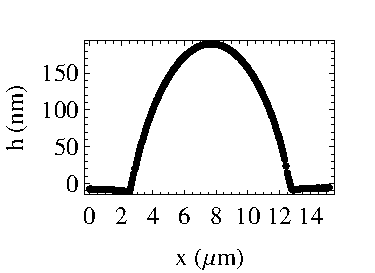
\includegraphics[scale=\totscale]{Figs_Friction/Section_SB03-2A.pdf}};
		\node at (0,-10 cm) {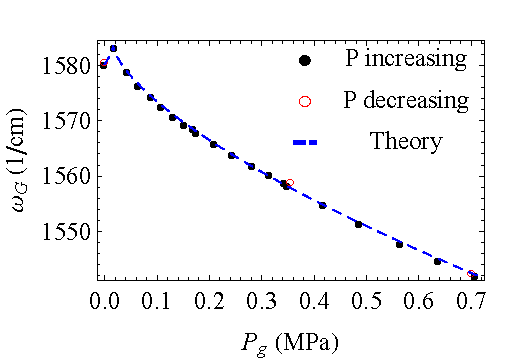
\includegraphics[scale=\totscale]{Figs_Friction/CenterFit_SB03-2A.pdf}};
	\end{scope}
	
	\node at (.7,1.75) [anchor=south west]{\textbf{b}  Snapped to side wall};
	\node at (-8,1.75) [anchor=south west]{\textbf{a} $P_0>P_a$};
\end{tikzpicture}
	\end{center}
	\caption{\label{fig:fri:ambient}Characteristic ambient pressure behavior of FLG sealed microchambers. Low contact force ($\approx 1\ nN$) AFM taken at ambient pressure with line cuts (top) and the center frequency of the single Lorentzian fit spectra taken at the center of the hole as a function of the applied gauge pressure (bottom) for (a) (left hand side) a $10 \ \mu m$ trilayer sealed microchamber and (b) (right hand side) a $6 \ \mu m$ monolayer sealed microchamber.}
\end{figure}

\section{Qualitative results}
The Raman line scans over pressurized microchambers show that the supported graphene around the microchamber has slid inward toward the center.
Figure \ref{fig:fri:qualresults} shows the G band center frequency of the fit Lorentzians plotted as a function of position across a $6 \ \mu m$ diameter monolayer covered graphene sealed microchamber with applied absolute pressures of 0.45 and 0.80 MPa during three separate pressure cycles from atmospheric to 0.80 MPa.
As expected, as the suspended graphene is pushed down into the microchamber, the G band red shifts or softens from its unstrained value.
Unexpectedly, the G band of the supported graphene \emph{outside} the edge of the microchamber also shows softening, and thus significant strain.
The observed softening decreases with the distance from the edge of the microchamber until the G band returns to its unstrained energy.
This strain is real; the G band red shift cannot be attributed to the averaging over the finite spot size of the beam because the measured downshifts persist much further from the edge of the microchamber than the $0.83 \ \mu m$ beam waist.
As the applied pressure increases, more strain is distributed outside of the microchamber causing both a larger redshift and a larger region over which the strain is distributed.
The strain distributed outside of the microchamber's edge is a clear indicator that the graphene is not rigidly fixed to the substrate outside of the microchamber.
Instead of a line force acting at the circumference of the microchamber to fix the graphene at the edge, there must be a distributed sliding frictional force, $f$, acting between the graphene and the substrate.

This behavior is reproducible, stable, and azimuthally symmetric.
The four 0.45 MPa line scans in Figure \ref{fig:fri:qualresults} include one line scan in the x direction for each of the first two pressure cycles and a line scan from both the x and y direction during the third pressure cycle.
The five 0.80 MPa line scans include one line scan in the x direction from the first pressure cycle, two sequential line scans in the x direction which took 35 minutes each from the second pressure cycle, and a line scan from both the x and y direction during the third pressure cycle.
Other than the development of a dimple at the center of the microchamber, the spectra and G band shifts are nearly identical.
This dimple is the result of laser deposition of dirt at the center of microchamber due to tens of hours of high pressure resolution, single point measurements.
This dirt seems to stabilize the graphene underneath, reducing the strain in its vicinity.
An SEM image of the schmutz dimple is shown in the inset.

\begin{figure}
	\begin{center}
	\begin{tikzpicture}[scale=1]
	%The spectra
	\node at (0,0) {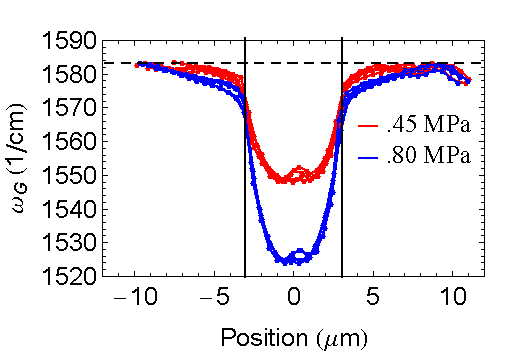
\includegraphics{Figs_Friction/QualLine.pdf}};
	
	%The picture of the hole
	\newcommand{\arrowlength}{1.5*.16*3.33 cm}
	\begin{scope}[xshift=-1.5 cm,yshift=0 cm]
		\node at (0,0) {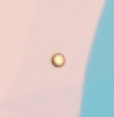
\includegraphics[scale=.75,angle=0,trim=9.75mm 8.5mm 8.5mm 10.25mm,clip]{Figs_Friction/SB02-3_cropped.jpg}};
		\draw[black,thick] (0,\arrowlength) -- (0,-\arrowlength) ;
		\draw[black,thick] (\arrowlength,0) -- (-\arrowlength,0);
	\end{scope}
	
	%The picture of the SEM dot
	\begin{scope}[xshift=2.6 cm,yshift=-.8 cm]
		\node at (0,0) {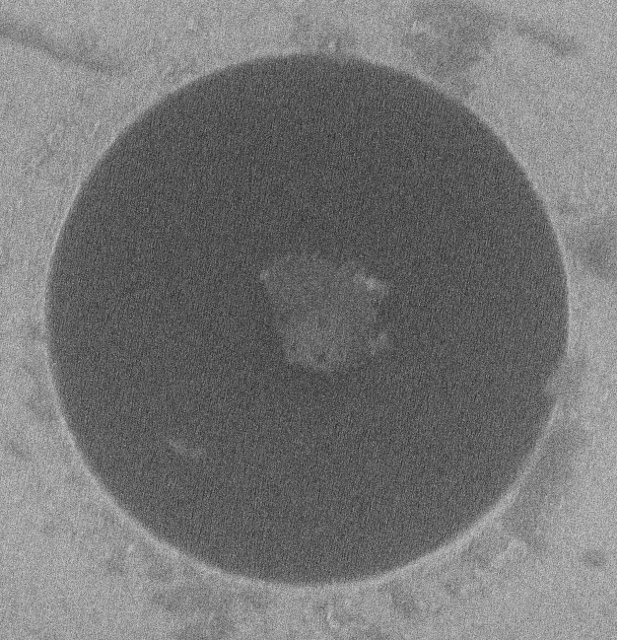
\includegraphics[width=.07 \textwidth]{Figs_Friction/SB02-3_05_SEM.jpg}};
	\end{scope}

\end{tikzpicture}
	\end{center}
	\caption{\label{fig:fri:qualresults}The frequency shift of the Raman G band as a function of position for four line scans taken at 0.45 MPa and five line scans taken at 0.80 MPa from 3 separate pressure cycles scanned across a single $6 \ \mu m$ diameter monolayer sealed microchamber. Inset left shows sample and line scan directions.  Each point represents the position of the center of a single Lorentzian fit to the Raman spectra at that position.  Solid vertical black lines are positioned at the edges of the microchamber and the dashed horizontal line indicates the zero strain position of the G band.  Data points are separated by $0.5 \ \mu m$; the focused beam has a waste of $0.81 \ \mu m$.  The bottom right inset is an SEM image of the device after all data acquisition showing the laser induced dirt deposited at the center of the microchamber.}
\end{figure}

To determine the nature of the strain outside of the microchamber, Raman spectra $2 \ \mu m$ outside the edge of a $10 \ \mu m$ diameter monolayer covered microchamber were analyzed in detail.
Circularly polarized spectra at this point show two discrete $G^+$ and $G^-$ peaks confirmed with linearly polarized spectra as shown in Figure \ref{fig:fri:qualout}.
The peak positions indicate a tensile radial strain of 0.6\% and a compressive tangential strain of -0.3\% at this location.
The compressive tangential strain is expected: when an annulus of the supported FLG is pulled inward, its circumference shrinks and, if the adhesion energy between FLG and its substrate is large enough to suppress out-of-plane wrinkling, this shrinkage causes compressive tangential strain.

In our Raman and AFM experiments we see no evidence of the FLG wrinkling to relieve its compressive strain.
As shown in Figure \ref{fig:fri:cylindrical}, a partial Raman map of this $10 \ \mu m$ diameter monolayer covered microchamber at 0.80 MPa shows a high degree of radial symmetry indicative of wrinkle free graphene.
To generate the Raman maps shown in Figure \ref{fig:fri:cylindrical}, Raman spectra were taken at each spatial location on the map.
Each spectra was fit with two Lorentzians with energies $\omega^+$ and $\omega^-$ and the best fit energies were plotted as a function of position.
The two Lorentzian fit matches the characteristic two peak shape of the supported graphene shown in Figure \ref{fig:fri:circlelinear} for $\rho=1.4$.
Both maps in Figure \ref{fig:fri:cylindrical} were scaled to emphasize the shifts in the supported graphene peak positions.
As a result, the more highly strained suspended graphene appears black in the maps.
The $\omega^-$ Raman map, (a), shows very high radial symmetry while the $\omega^+$ map, (b), has slightly reduced symmetry.  At the highest point on the microchamber, there is a variation of around four wavenumbers in the $\omega^+$ map which could be due to small variations in local adhesion or doping.
The degree of radial symmetry exhibited by both of these Raman maps is a strong indicator that the supported graphene is not wrinkling.
Since these Raman maps are for the microchamber with the largest diameter and thinnest thickness at the highest applied pressure, the compressive strains are the highest of any of the microchambers measured.
Thus, we can rule out wrinkling for our other microchambers which have lower compressive strain.

\begin{figure}
	\begin{center}
	\newcommand{\sscale}{.6}
\newcommand{\sscaler}{.3}
\begin{tikzpicture}[scale=\sscale]	
	%The picture of the hole with the desciption of phiin and phoout
	\newcommand{\arrowlength}{1 cm}
	\begin{scope}[xshift=-4 cm,yshift=0 cm]
		%The spectra
		\node at (0,0) {\includegraphics[scale=\sscale]{Figs_Friction/PolarForSi.pdf}};
		%The hole
		\newcommand{\hcent}{1 cm}
		\begin{scope}[xshift=-.9 cm,yshift=10.15 cm,>=stealth]
			\node at (0,0) {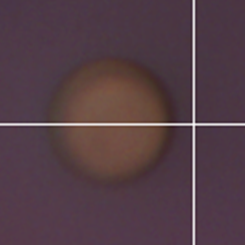
\includegraphics[scale=\sscaler ]{Figs_Friction/PolarPicture.png}};
			\draw[red,ultra thick,->] (\hcent-\arrowlength/2,-.03 cm) -- +(\arrowlength,0)  node[anchor=south west,fill=white]{$\phi_{in}$};
			\draw[green,ultra thick,->] (\hcent,-.03 cm) +(45:-\arrowlength/2) -- +(45:\arrowlength/2) node[anchor=south east, fill=white]{$\phi_{out}$};
		\end{scope}
	\end{scope}
	
	%The figure of the oscillating areas
	\begin{scope}[xshift=4 cm,yshift=0 cm]
		\node at (0,0) {\includegraphics[scale=\sscale]{Figs_Friction/ForSi_Areas.pdf}};
	\end{scope}
	
	\node at (.7,3) {\textbf{b}};
	\node at (-7,12.5) {\textbf{a}};
\end{tikzpicture}
	\end{center}
	\caption{\label{fig:fri:qualout} Linearly polarized Raman spectra of supported graphene.  (a) Spectra taken $2 \ \mu m$ outside a $5 \ \mu m$ radius graphene sealed microchamber pressurized to 0.80 MPa absolute pressure with the incident light polarized in the $\hat x$ direction ($\phi=0$) and the outgoing light linearly analyzed from -88 to 92 degrees in 20 degree steps.  The two peaks centered at $1570.9 \ 1/cm$ and $1581.3 \ 1/cm$ are selected by rotating the outgoing analyzer.  (b) The areas under the $1570.9 \ 1/cm$ and the $1581.3 \ 1/cm$ peak are shown as a function of outgoing analyzer angle in black and red, respectively.  The two data sets are fit with $\pi$ out-of-phase sine squared functions illustrating the expected orthogonality of the $G^+$ and $G^-$ peaks\cite{Huang2009}. The peak positions indicate a tensile radial strain of 0.6\% and a compressive tangential strain of -0.3\% at this location.}
\end{figure}

\begin{figure}
	\begin{center}
	\begin{tikzpicture}
	\node at (-4.75,2.75+5.5) {\textbf{(a)} $\omega^-$};
	\node at (0,5.5) {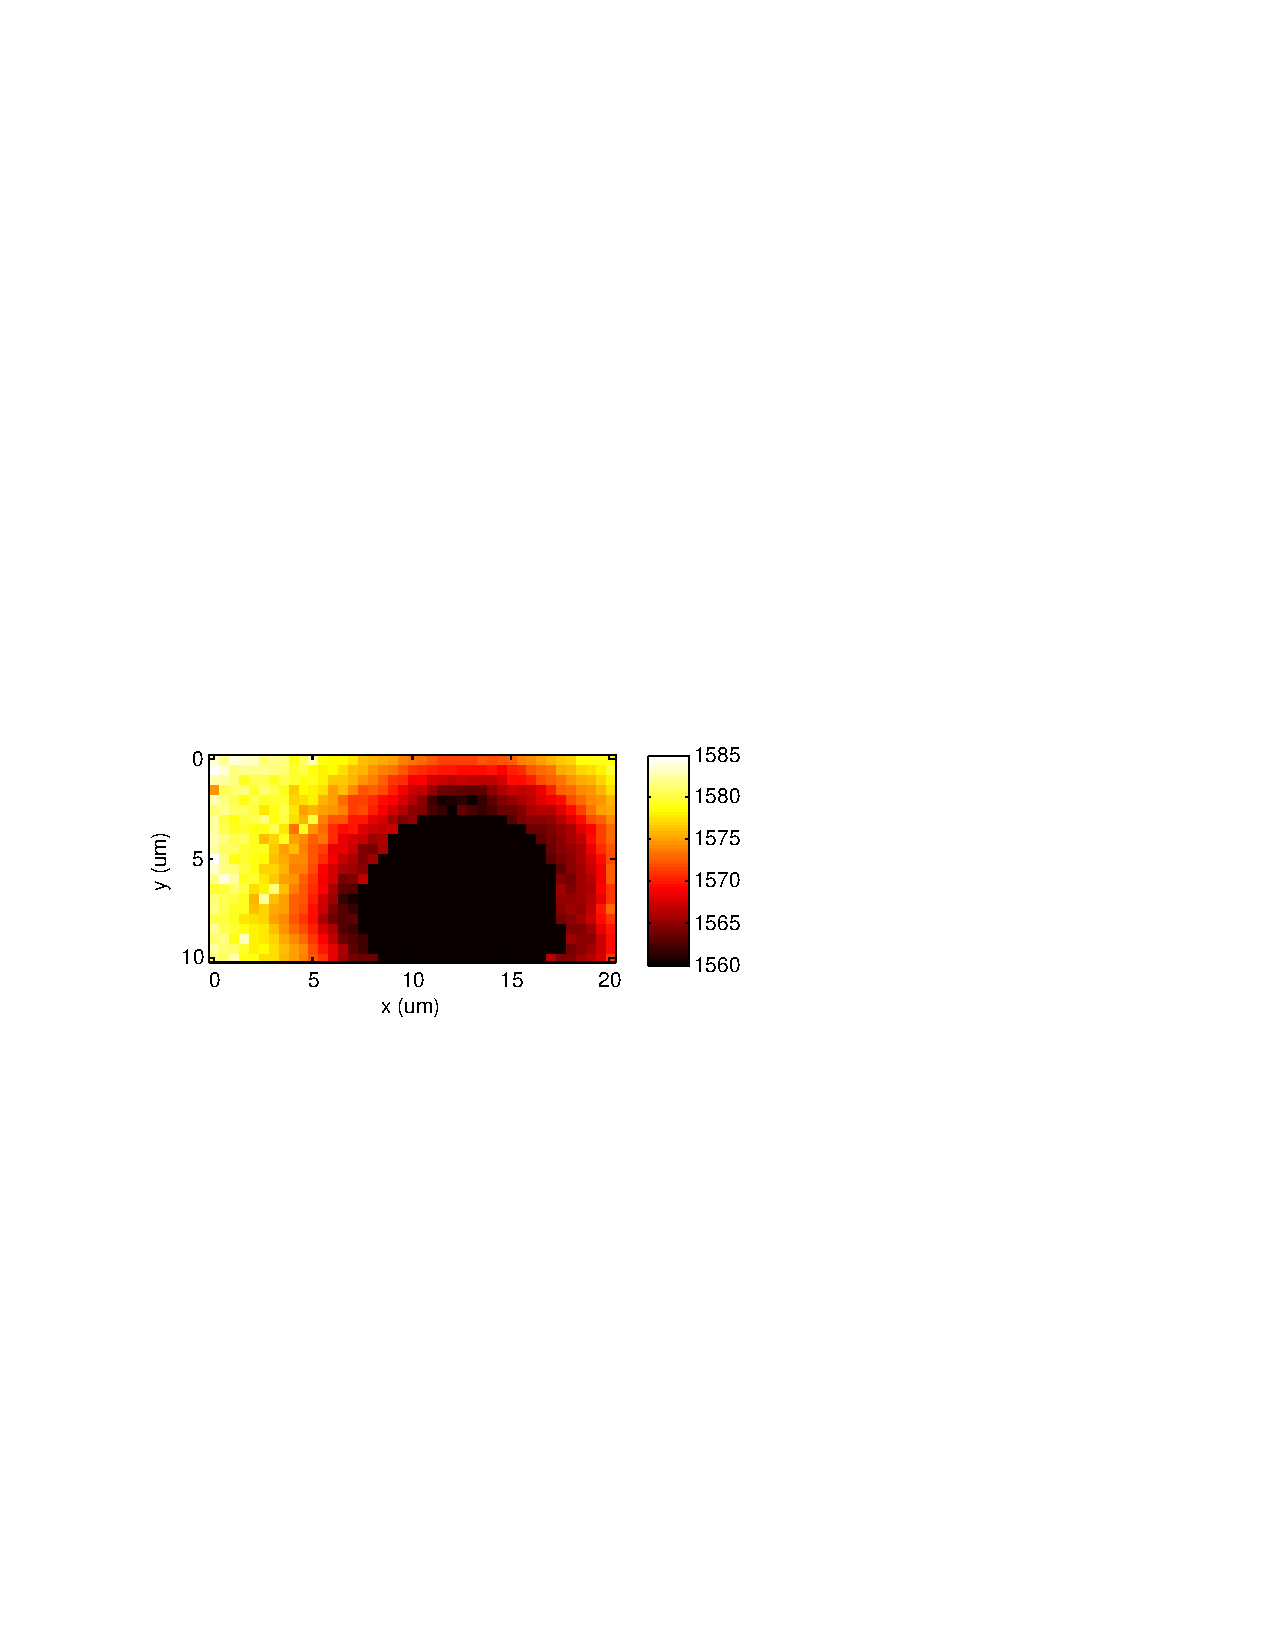
\includegraphics[scale=1]{Figs_Friction/x2.pdf}};
	\node at (-4.75,2.75) {\textbf{(b)} $\omega^+$};
	\node at (-.065,-.08) {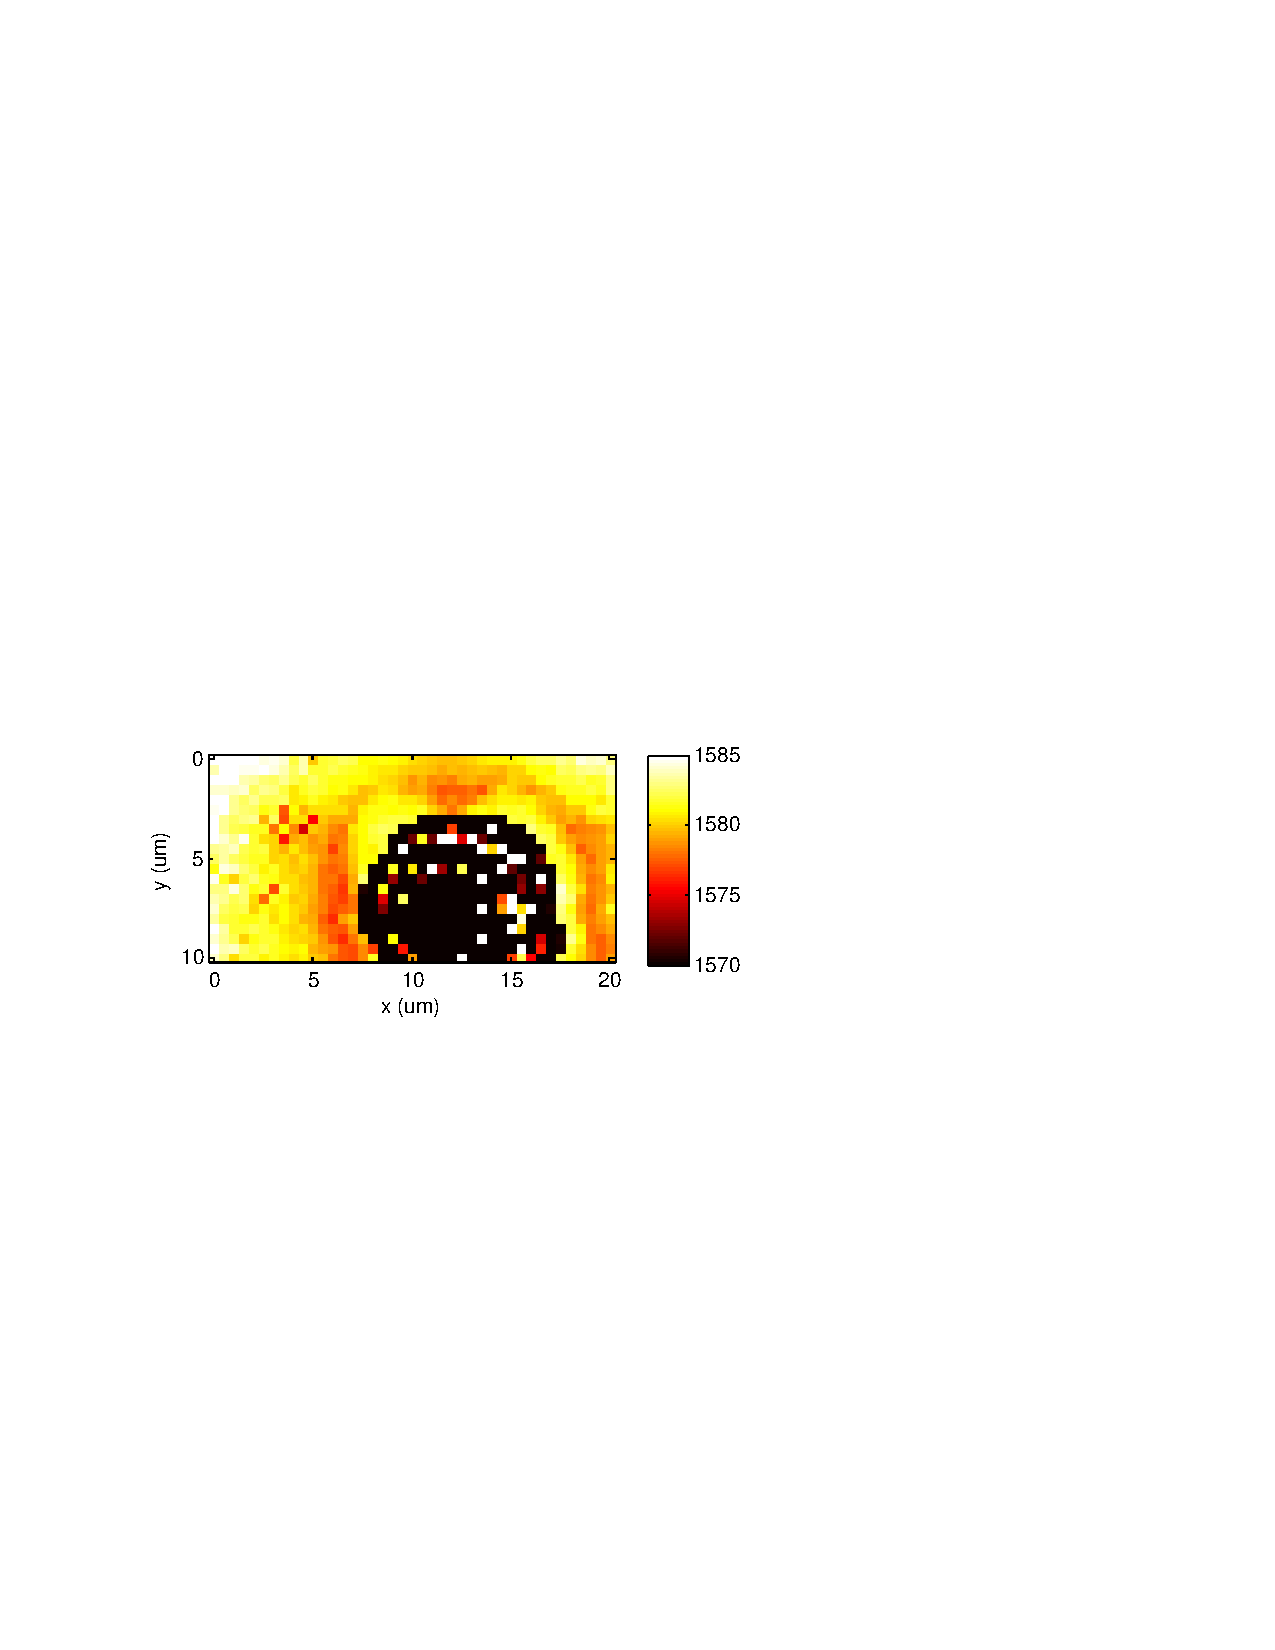
\includegraphics[scale=1]{Figs_Friction/x3.pdf}};
\end{tikzpicture}
	\end{center}
	\caption{\label{fig:fri:cylindrical} Raman map of (a) the $\omega^+$ peak and (b) $\omega^-$ peak for a $5 \ \mu m$ radii graphene sealed microchamber pressurized to 0.80 MPa.  In both maps the color scale is set to emphasize the peak shifts experienced by the supported graphene.  The speckles in (b) appear because the suspended graphene spectra are not fit well by two Lorentzians.  Both maps show a high degree of radial symmetry inconsistent with the formation of wrinkles.}
\end{figure}

\section{Continuum model of strain distributions}
We have developed a continuum model to extract the sliding friction, $f$, from the Raman determined strain distributions.
In 1915, Hencky proposed a continuum model for the non-linear pressure induced deflection of a thin circular plate with fixed boundary conditions \cite{Hencky1915,Fichter1997}.
This model has been successfully used to describe a variety of systems including inflatable membrane mirrors\cite{Meinel2000}, electrostatic actuators for micro gas pumps\cite{Zhang2011b}, and the topography of FLG bulging from sealed microchambers\cite{Koenig2011}.
The fixed boundary conditions assumed by this model preclude its application to the strain distributions that we observe.
However, we are able to relax the fixed boundary conditions and extend the Hencky model by matching the radial and tangential stresses inside the hole, derived from Hencky's model before the application of boundary conditions, to the radial and tangential stresses of the supported material outside of the hole calculated by including a sliding friction, $f$, acting against the radial displacement.
The stresses and, using Hooke's law, the strains, are then fully determined as a function of $\frac{\Delta P^2 E_{2D}}{f^3 R}$ where $R$ is the radius of the microchamber measured by AFM, $\Delta P$ is the differential pressure, and $E_{2D}$ is the 2D Young's modulus of FLG taken to be $n \times 340 \ N/m$ where n is the number of layers\cite{Lee2008,Koenig2011}.
A full derivation is included in the next section for those interested.
Figure \ref{fig:fri:theory} compares the radial and tangential strains from the standard Hencky solution, our extended Hencky solution and an atomistic, molecular dynamics model.
The solid lines of our extended model demonstrate the desired features; strain is distributed \emph{outside} of the hole with compressive tangential, and tensile radial strain.
The strain distribution depends on the friction as expected: At constant pressure and radius, a greater sliding friction holds the graphene more firmly to the substrate surrounding the hole, and thereby increases $\epsilon_c$, the strain in the center of the microchamber while also reducing $\rho_0$, the largest radial distance that the strain is acting outside of the hole.
Our extended model, with f=520 MPa, is in good agreement with the dots in Figure \ref{fig:fri:theory} that are the results of an atomistic molecular dynamics simulation of a 6 nm radius microchamber under 500 MPa of pressure performed using the open source simulation package LAMMPS~\cite{plimptonLAMMPS,PlimptonJCP1995} developed at Sandia National Labs.
A detailed description of the atomistic modeling is included below for those interested.
To our knowledge, this is the first time that Hencky's model has been generalized to allow strain to be distributed outside of the microchamber's edge.

\begin{figure}
	\begin{center}
	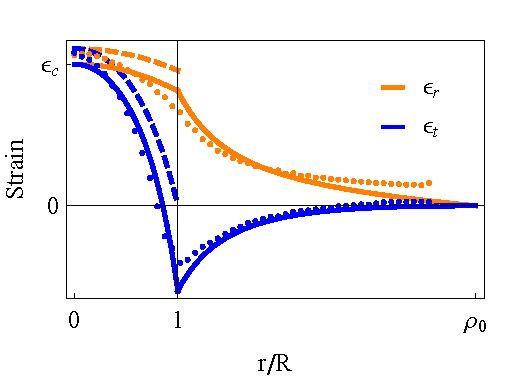
\includegraphics{Figs_Friction/Figure_3.pdf}
	\end{center}
	\caption{\label{fig:fri:theory} Theoretical strains in few layer graphene sealed microchambers. Comparisons of the radial and tangential strains predicted by Hencky's model (dashed), our extended Hencky model that includes strain outside the microchamber for a sliding friction of f=520 MPa (solid), and atomistic simulations of a 6 nm radius microchamber with 500 MPa of applied pressure (dots). The extended Hencky model used to extract friction agrees very well with the atomistic model.}
\end{figure}

\subsection{Detailed derivation of the extended Hencky model}
Throughout this section we treat graphene in the continuum limit as a thin plate: A solid which is much thinner in one dimension than the other two.
The Hencky model \cite{Hencky1915,Fichter1997} is a series solution for the pressure induced deflection of a thin circular plate with fixed boundary conditions.
Here we extend the model to allow strain to be distributed outside of the edges of the hole.
Instead of applying fixed boundary conditions at the edge of the hole, the radial and tangential stresses inside the hole are matched to the radial and tangential stresses experienced by the material being pulled into the hole.
This fully defines the strain in the system as a function of the dimensionless loading parameter, $q=\frac{\Delta PR}{E_{2D}}$, and the dimensionless friction coefficient $F=Rf/E_{2D}$ in the combination $q^{2/3}/F$.
Large dimensionless loading, $q^{2/3}$, causes the same effects as  small friction, $F$;  pulling hard has the same effect as sliding easily.
Here $\Delta P$ is the pressure differential over the plate, $R$ is the radius of the hole, and $E_{2D}$ is the product of the Young's modulus and the thickness of the plate.
A simple analytic relationship does not exist between  $q^{2/3}/F$ and the two parameters which define the shape of the strain profile: the distance over which the strain spreads outside of the hole, $\rho_0$, and the coefficient of stress at the center of the hole, $b_0$.
However, these can easily be solved for analytically.
To find solutions to our extended Hencky model the general forms of the stress inside and outside of the hole will be derived, and then the boundary condition will be determined and applied.

Assuming that there is no shear, the stress-strain relationship for the thin plate is the same inside and outside the hole\cite{Landau1986}:
\begin{align}
	\epsilon_r&=\sigma_r-\nu \sigma_t \label{eq:fri:esr}\\
	\epsilon_t&=\sigma_t-\nu \sigma_r \label{eq:fri:est}
\end{align}
where $\nu$ is the Poisson Ratio and $\sigma_r$ and $\sigma_t$ are the dimensionless radial and tangential stresses given by the stress divided by the Young's modulus.

Both the strain-displacement and the governing equations, however, depend on the region of interest.
Inside the hole the plate flexes down into the hole as pressure is applied.
The resulting strain-displacement relationships are:
\begin{align}
	\epsilon_r^i&=\frac{dU}{d\rho}+\frac{1}{2} (\frac{dW}{d\rho})^2 \label{eq:fri:edri}\\
	\epsilon_t^i&=\frac{U}{\rho} \label{eq:fri:edti}
\end{align}
here $U$ is the dimensionless radial deflection, $W$ is the dimensionless out of plane deflection, and $\rho$ is the dimensionless radius, all of which are made dimensionless by dividing by the radius of the hole.
The governing equations inside the hole are calculated by balancing the forces on a radial element.
The stresses and pressure acting on such an element are shown in Figure \ref{fig:fri:stressfigurei}.
\begin{figure}
	\begin{center}
	\newcommand{\halfangle}{10}
\begin{tikzpicture}[scale=2]
	%The radial equilibrium
	\begin{scope}[xshift=-4.5 cm]
		%The bisected dotted lines
		\begin{scope}[dashed,gray,very thin]
			\draw (0,0) -- (\halfangle:1.5 cm);
			\draw (0,0) -- (-\halfangle:1.5 cm);
		\end{scope}
		%Draw the area element
		\filldraw[fill=gray!10,draw=black] (-\halfangle:1.5 cm)  arc(-\halfangle:\halfangle:1.5 cm) -- (\halfangle:2 cm) arc(\halfangle:-\halfangle:2 cm) -- cycle;
		%Draw the force lines and labels
		\begin{scope}[->, blue!50!black,>=stealth]
			\draw (0:2 cm) -- +(0:.25 cm) node[anchor=west]{$N_r+\frac{dN_r}{dr} dr$};
			\draw (0:1.5 cm) -- +(0:-.25 cm) node[anchor=east]{$N_r$};
			\draw (\halfangle:1.75 cm) -- +(90+\halfangle:.25 cm) node[anchor=south east]{$N_t$};
			\draw (-\halfangle:1.75 cm) -- +(-90-\halfangle:.25 cm) node[anchor=north east]{$N_t$};
		\end{scope}
		\draw (.25,.75 cm) node{Top:};
	\end{scope}
	
	%The lateral equilibrium
	\begin{scope}[->, blue!50!black,>=stealth]
		\draw (0,0) -- (20:-.25 cm) node[anchor=north east]{$N_r$};
		\draw[black,thick,-] (20:0 cm) -- ++(20:.5 cm);
		\draw (20:.5 cm)  -- ++(20:.25 cm) node[anchor=west]{$N_r+\frac{dN_r}{dr} dr$};
		\draw (20:.25 cm) -- ++(90:.25 cm) node[anchor=west]{$P$};
		\filldraw (0,0) circle(.5pt);
		\filldraw (20:.5 cm) circle(.5pt);
		\filldraw (20:.25 cm) circle(.5pt);
	\end{scope}
	\draw (-.25,.75 cm) node{Side:};
	
\end{tikzpicture}
	\end{center}
	\caption{\label{fig:fri:stressfigurei}The stresses, $N_r$ and $N_t$, and pressure, $P$ acting on a radial area element for $\rho<1$ as viewed from the top and side.}
\end{figure}
Using the area of the radial element ($r dr d\theta$) to convert the pressure to a force, and the cross sectional area to convert the strains into forces results in the two governing equations:
\begin{align}
	\sigma_t^i&=\frac{d}{d \rho}(\rho \sigma_r^i) \label{eq:fri:g1i}\\
	\sigma_r^i \frac{dW}{d \rho}&=-\rho \frac{q}{2} \label{eq:fri:g2i}
\end{align}
the first from radial equilibrium and the second from lateral equilibrium with $\sigma_r$ and $\sigma_t$ the radial and tangential stresses, $N_r$ and $N_t$, divided by the Young's modulus to make them dimensionless.
These six equations can be combined to form a single differential equation for $\sigma_r$:
\begin{equation}
	\frac{1}{8} \rho q^2+ (\sigma_r^i)^2 \frac{d}{d\rho}[\sigma_r^i+\frac{d}{d\rho}(\rho \sigma_r^i)]=0
	\label{eq:fri:comboin}
\end{equation}
This is most easily found by using eqn. \ref{eq:fri:g1i} and then eqn. \ref{eq:fri:g2i} in the combination of equations: $[(\ref{eq:fri:edri}) \rightarrow (\ref{eq:fri:esr})]-\frac{d}{d \rho}\rho[(\ref{eq:fri:edti})\rightarrow(\ref{eq:fri:est})]$.
Solving this equation for $\sigma_r$ determines $\sigma_t$, $\epsilon_r$, and $\epsilon_t$ using equations \ref{eq:fri:g1i}, \ref{eq:fri:esr}, and \ref{eq:fri:est}.
Since there is no analytic solution to this differential equation, we follow Hencky and assume a series expansion of the radial stress even in powers of $\rho$ to match symmetry:
\begin{equation}
	\sigma_r^i=\frac{1}{4} q^{2/3} \sum_{n=0}^{\infty} b_{2n} \rho^{2n}
\end{equation}
When used in eqn. \ref{eq:fri:comboin} all of the higher order coefficients are determined in terms of one free parameter, $b_0$, the stress coefficient at the center of the hole.
To this point the derivation has not deviated from Hencky's original work.
However, instead of continuing forward to determine the value of $b_0$ by requiring that there is no radial deflection at the edge of the hole, $b_0$ will be left as a free parameter to match to the strain outside of the hole, which we now derive.

Outside of the hole the plate is constrained to move in the x-y plane, radial symmetry is preserved, and friction is present. 
The stress strain relationships (eqns. \ref{eq:fri:esr} and \ref{eq:fri:est}) are for a thin plate with no shear, and thus, apply equally well outside the hole as inside.
The strain displacement relationships are based on the geometry of a general radially symmetric differential element.
The only change that needs to be made to these is the elimination of the out of plane motion:
\begin{align}
	\epsilon_r^o&=\frac{dU}{d\rho} \label{eq:fri:edro}\\
	\epsilon_t^o&=\frac{U}{\rho} \label{eq:fri:edto}
\end{align}
For sufficiently negative $\epsilon_t$, the plate is expected to buckle out-of-plane, forming wrinkles.
However, in our experimental regime we do not see evidence for these effects.
The forces acting on the plate are different inside and outside the hole, and thus, so are the governing equations.
The stresses and forces acting on the graphene outside of the hole are shown in Figure \ref{fig:fri:stressfigureo}.
\begin{figure}
	\begin{center}
	\newcommand{\halfangle}{10}
\begin{tikzpicture}[scale=2]
	%The bisected dotted lines
	\begin{scope}[dashed,gray,very thin]
		\draw (0,0) -- (\halfangle:1.5 cm);
		\draw (0,0) -- (-\halfangle:1.5 cm);
	\end{scope}
	%Draw the area element
	\filldraw[fill=gray!10,draw=black] (-\halfangle:1.5 cm)  arc(-\halfangle:\halfangle:1.5 cm) -- (\halfangle:2 cm) arc(\halfangle:-\halfangle:2 cm) -- cycle;
	%Draw the force lines and labels
	\begin{scope}[->, blue!50!black,>=stealth]
		\draw (0:2 cm) -- +(0:.25 cm) node[anchor=west]{$N_r+\frac{dN_r}{dr} dr$};
		\draw (0:1.5 cm) -- +(0:-.25 cm) node[anchor=east]{$N_r$};
		\draw (\halfangle:1.75 cm) -- +(90+\halfangle:.25 cm) node[anchor=south east]{$N_t$};
		\draw (-\halfangle:1.75 cm) -- +(-90-\halfangle:.25 cm) node[anchor=north east]{$N_t$};
		\filldraw[red!40!black] (1.75,0) circle(.5pt);
		\draw[red!40!black] (1.75,0) -- +(.15,0) node[anchor=south east]{$f$};
	\end{scope}
\end{tikzpicture}
	\end{center}
	\caption{\label{fig:fri:stressfigureo}The stresses, $N_r$ and $N_t$, and friction, $f$, on a radial area element for $\rho>1$.}
\end{figure}
The interaction between the plate and its underlying substrate is included via the frictional force per unit area, $f$, which is pointed to oppose the stresses outside of the hole.
Care needs to be taken in this mathematical treatment because this friction term does not turn off when the stress goes to zero.
Instead, it works in positive feedback amplifying the stress. 
As a result, the stresses are only physical until they decay to zero at a position $\rho_0$.
If there were a component of friction acting against the tangential strain, it would go as $d \theta^2$, one power for the resultant and one power for the area element, rendering it negligible.
The governing equation outside the hole is then:
\begin{equation}
	\sigma_t^o=\frac{d}{d\rho}(\rho \sigma_r^o)+F \rho
	\label{eq:fri:g1o}
\end{equation}
Again these equations can be combined to form a single differential equation for $\sigma_r$.
The easiest way to do this is by using eqn. \ref{eq:fri:g1o} twice in the combination of equations: $[(\ref{eq:fri:edro}) \rightarrow (\ref{eq:fri:esr})]-\frac{d}{d \rho}\rho[(\ref{eq:fri:edto})\rightarrow(\ref{eq:fri:est})]$.
The result is:
\begin{equation}
	\frac{d}{d\rho}[\sigma_r^o+\frac{d}{d\rho}(\rho \sigma_r^o)]=-(2+\nu) F
	\label{eq:fri:comboout}
\end{equation}
Unlike the situation inside of the hole, this equation can be solved exactly.  The general result for the radial and tangential stress (eqn. \ref{eq:fri:g1o}) are:
\begin{align}
	\sigma_r^o&=(2+\nu)F(-\frac{\rho}{3}-\frac{c_2}{2 \rho^2})+c_1 \\
	\sigma_t^o&=(2+\nu)F(-\rho \frac{1+2 \nu}{3(2+\nu)}+\frac{c_2}{2 \rho^2})+c_1
\end{align}
Usually, it would be natural to restrict this solution by requiring that the strain at $\rho=\infty$ goes to zero.
In this case, this cannot be done because of the unphysical form of the strain for positions $\rho>\rho_0$.
Instead, the radial and tangential strains are forced to both go to zero at the position $\rho_0$.
This gives $c_2=\rho_0^3 \frac{\nu-1}{3(2+\nu)}$ and $c_1=\rho_0 \frac{1+\nu}{2} F$, completely defining the strains outside in closed form as a function of one free parameter, $\rho_0$, which defines the furthest reach of the stress outside of the hole.

Having determined the stresses inside and outside of the hole, the boundary condition for the stresses at the edge of the hole will be determined.
The stress is related to the force per unit area through a divergence operation:
\begin{equation}
	F_i=\frac{\partial N_{ik}}{\partial x_k}
\end{equation}
where $F_i$ is the force per unit volume in the $i$ direction, $N_{ik}$ is the strain tensor, and repeated indices are summed over.
Integrating the equations and using the divergence theorem gives:
\begin{equation}
	\int_V F_i \ dV=\oint_S \sigma_{ik} \ df_k
\end{equation}
The total force acting on a volume entity is given by the surface integral of the stress.
A symmeterized volume element that spans the edge of the hole is shown in Figure \ref{fig:fri:egestress}.
In the limit that $\epsilon \rightarrow 0$ the distributed surface forces $f$ and $P$ contribute nothing to the force on this volume element, forcing the left hand side to zero.
This would not be the case if these were 1D edge forces.
The undrawn tangential stresses also go to zero as the cross section that they act on, $\epsilon h$, goes to zero as well. 
Thus, the remaining stresses must be equal:
\begin{equation}
	N_r^i=N_r^o
\end{equation}
The boundary condition on the tangential stress is found by the requirement that the radial displacement, $U$, must be continuous.
If it were not, the material on one side of the discontinuity would separate from the material on the other side leaving a gap.
If $U$ is continuous, so must $\epsilon_t$ be by eqns. \ref{eq:fri:edti} and \ref{eq:fri:edto}.
Finally, if $\epsilon_t$ and $N_r$ are continuous, so must $N_t$ be by equation \ref{eq:fri:est}.
Thus, we have shown that the radial and tangential stresses must be continuous over the edge of the hole.

\begin{figure}
	\begin{center}
	\newcommand{\halfangle}{10}
\newcommand{\dr}{.3 cm}
\newcommand{\rbeg}{1.5 cm}
\newcommand{\Larrow}{.25 cm}
\begin{tikzpicture}[scale=2]
	%The bisected dotted lines
	\begin{scope}[dashed,gray,very thin]
		\draw (0,0) -- (\halfangle:\rbeg);
		\draw (0,0) -- (-\halfangle:\rbeg);
	\end{scope}
	%Draw the area element
	\filldraw[fill=gray!10,draw=black] (-\halfangle:\rbeg)  arc(-\halfangle:\halfangle:\rbeg) -- (\halfangle:\rbeg+\dr) arc(\halfangle:-\halfangle:\rbeg+\dr) -- cycle;
	%Draw the edge of the hole
	\draw[dotted,thick] (-4*\halfangle:\rbeg+\dr/2) arc(-4*\halfangle:4*\halfangle:\rbeg+\dr/2) node[anchor=south]{$\rho=1$};
	%Draw the force lines and labels
	\begin{scope}[->, blue!50!black,>=stealth]
		\draw (0:\rbeg+\dr) -- +(0:\Larrow) node[anchor=west]{$N_r^o$};
		\draw (0:\rbeg) -- +(0:-\Larrow) node[anchor=east]{$N_r^i$};
		\filldraw[red!40!black] (\rbeg+\dr*3/4,0) circle(.5pt);
		\draw[red!40!black] (\rbeg+\dr*3/4,0) -- +(.1,0) node[anchor=south east]{$f$};
		\filldraw[red!40!black] (\rbeg+\dr*1/4,0) circle(.5pt) node[anchor=north]{$P$};
	\end{scope}
	%Draw the width of the element
	\draw[<->,black,>=stealth] (\halfangle*5/4:\rbeg) -- node[anchor=south]{$\epsilon \rightarrow 0$} +(\halfangle*5/4:\dr);
\end{tikzpicture}
	\end{center}
	\caption{\label{fig:fri:egestress}The stresses and forces acting on a thin, symmetrized volume element which spans the edge of the hole.  The tangential strains inside and outside are ignored as their contribution goes to zero as $\epsilon \rightarrow 0$.}
\end{figure}

With a series solution for the stresses inside the hole with the stress at the center of the hole, $b_0$, as a free parameter, and with a closed form solution for the stresses outside of the hole with the furthest distance the stress spreads, $\rho_0$, as a free parameter, we can match the stresses with the boundary condition to uniquely define the stresses in terms of $q$ and $\mu$.
We use the continuity of the radial and tangential stresses at the boundary to solve for our two free parameters $\rho_0$ and $b_0$.
\begin{align*}
	\sigma_r^i(\rho=1)&=\sigma_r^o(\rho=1) \\
	\sigma_t^i(\rho=1)&=\sigma_t^o(\rho=1) 
\end{align*}
This sets the value of $\rho_0$ and $b_0$ in terms of $q^{2/3}/F$.
Regrettably, the series form of the solution inside of the hole makes the presentation of an exact expression for $\rho_0$ and $b_0$ impossible.
Numerical solutions for the values of $\rho_0$ and $b_0$ are presented in Figures \ref{fig:fri:rho0} and \ref{fig:fri:b0} for graphite's Poisson ratio of 0.165\cite{Blakslee1970}.
As the friction increases or the dimensionless loading coefficient decreases, $q^{2/3}/F$ decreases, and $\rho_0$ decreases toward unity, the value for no strain distribution outside of the hole, while $b_0$ increases toward 1.66, the result of the Hencky model. 

\begin{figure}
	\begin{center}
	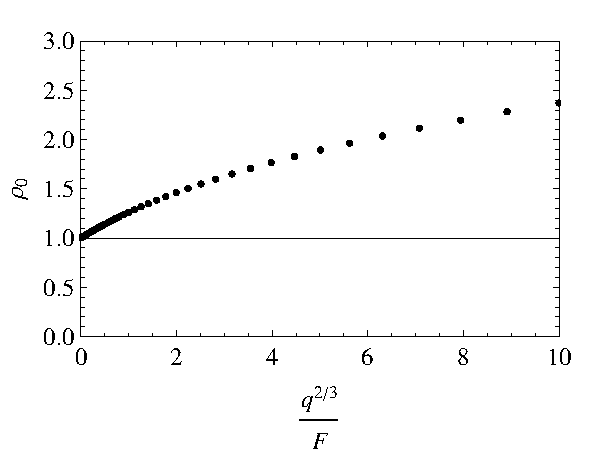
\includegraphics{Figs_Friction/rho0.pdf}
	\end{center}
	\caption{\label{fig:fri:rho0} Numerical solutions for values of $\rho_0$. Note convergence to $\rho_0 = 1$ as the dimensionless loading decreases or the friction increases, corresponding to no stress distributed outside of the hole.}
\end{figure}

\begin{figure}
	\begin{center}
	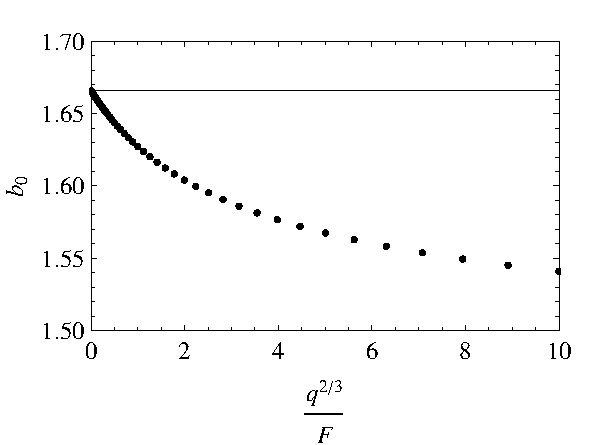
\includegraphics{Figs_Friction/b0.pdf}
	\end{center}
	\caption{\label{fig:fri:b0} Numerical solutions for values of $b_0$. Note the convergence to the value 1.66 for small loading (or large friction), approaching the result of the Hencky model.}
\end{figure}

\subsection{Detailed derivation of Atomistic model}
Classical molecular dynamics simulations (MD) were performed using open source simulation package LAMMPS~\cite{plimptonLAMMPS,PlimptonJCP1995} developed at Sandia National Labs to investigate the atomistic details underlying the experimental results.
The model used argon gas to compress a graphene monolayer that lies atop an amorphous silicon dioxide substrate, as illustrated in Figure \ref{fig:fri:MD}.
The substrate had dimensions 46 x 46 x 3 nm with a 6 nm radius hole in the center.
A circular graphene monolayer with radius 22 nm was placed on top of the hole in the substrate and argon atoms were randomly distributed within the simulation box after relaxation of the graphene-substrate system.
There were 562,110 atoms in total, with the simulation run in parallel for maximum computational efficiency.

The covalent carbon bonds were modeled using the AIREBO\cite{stuartJCP2000} potential, which has been shown to have good accuracy in describing hydrocarbon systems~\cite{qiNANO2010,zhaoJAP2010}.
The Tersoff~\cite{tersoffPRB1988} potential was utilized for the Si-Si, Si-O and O-O interactions, while a Lenard-Jones potential was used for all other interactions with a cutoff distance of 8\AA \ and the corresponding interaction parameters chosen as follows: $\epsilon_{Ar-Ar}$=0.0104eV, $\sigma_{Ar-Ar}$=3.405\AA~\cite{RytkonenJchemp1998}; $\epsilon_{Ar-C}$=0.0123eV, $\sigma_{Ar-C}$=3.573\AA~\cite{RobertNano1996};$\epsilon_{Ar-Si}$=0.0028eV, $\sigma_{Ar-Si}$=3.778\AA~\cite{LiPRA2010}; $\epsilon_{Ar-O}$=0.0058eV, $\sigma_{Ar-O}$=3.3075\AA~\cite{EverittJCP1999}; $\epsilon_{Si-C}$=0.008909eV, $\sigma_{Si-C}$=3.326\AA~\cite{OngPRB2010}; $\epsilon_{O-C}$=0.003442eV, $\sigma_{O-C}$=3.001\AA~\cite{OngPRB2010}.
The Ar-Si and Ar-O interaction parameters were obtained using the standard Lorentz-Berthelot mixing rule.

\begin{figure}
	\begin{center}
	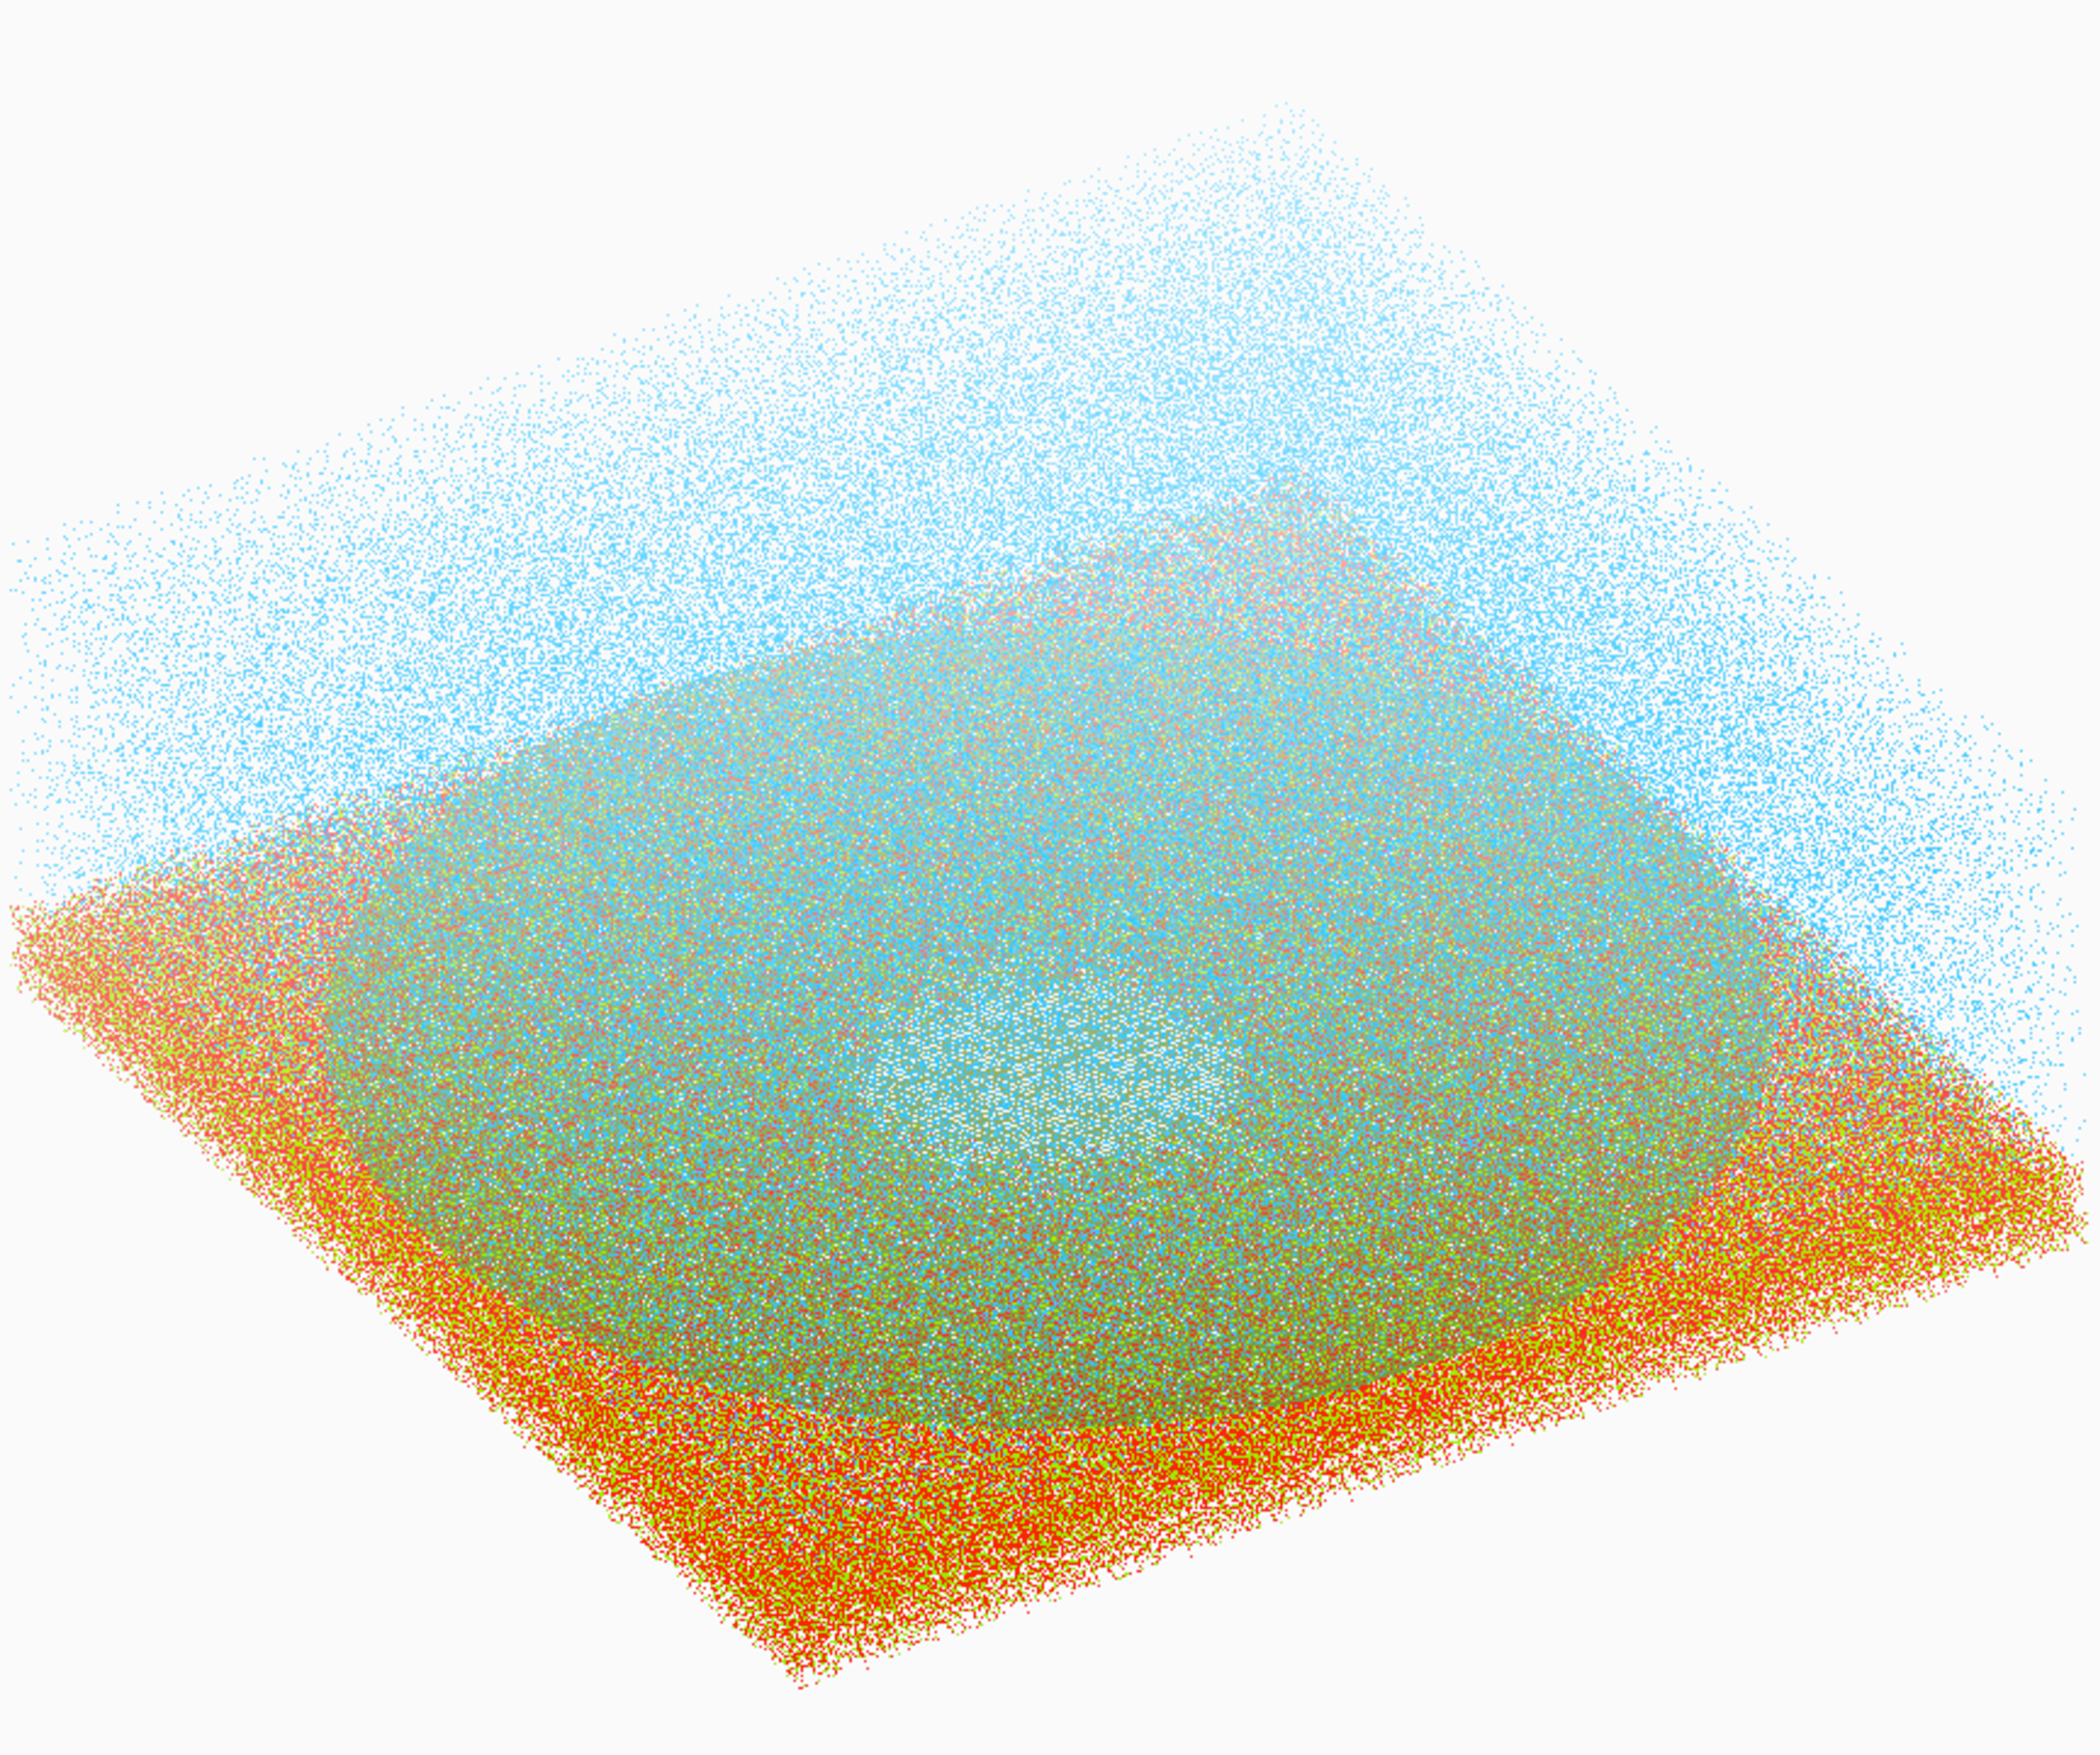
\includegraphics[scale=0.15]{Figs_Friction/MD.pdf}
	\end{center}
	\caption{\label{fig:fri:MD} Schematic diagram of the simulation system including (from bottom to top) amorphous SiO$_{2}$ substrate (red and orange atoms), circular graphene monolayer (brown atoms) and argon gas (cyan atoms). Visualization was performed using Visual Molecular Dynamics~\cite{Humphrey1996}.}
\end{figure}

The system was first relaxed at room temperature (300K) for .03 MPa, at which point the gas density was slowly increased by reducing the volume of gas to increase the pressure.
When the desired deflection of graphene was reached, the gas density was then kept fixed, and the system was allowed to relax at that pressure for 10 ps.
The final equilibrium configuration of graphene was computed by averaging over all of the atomic positions of graphene during the relaxation period with constant gas density.
The substrate was assumed to be rigid and fixed during the simulation.
As a boundary condition on the graphene, the atoms in the outer 1 nm annulus of the supported graphene were fixed during the simulation matching the experimental observation that the supported graphene only slides in a local region around the hole, remaining fixed at large radii.
A canonical ensemble (NVT) with room temperature (300K) was used for the entire simulation and reflection boundary conditions were used to ensure that gas atoms remained inside the simulation box.  

To calculate the strain in the deformed graphene sheet, we first calculated the atomistic displacement field~\cite{ZimmermanIJSS2009} by calculating the difference between the reference (initial) configuration and the final, deformed configuration.
The strain tensor from continuum mechanics was then calculated as
\begin{equation} \label{eq:fri:straindisp}
	\epsilon_{ij}=\frac{1}{2}\left(\frac{\partial {u_i}}{\partial {X_j}} + \frac{\partial {u_j}}{\partial {X_i}} + \frac{\partial{u_k}\partial{u_k}}{\partial{X_i}\partial{X_j}}\right),
\end{equation}
where $\epsilon_{ij}$ are the components of the strain, $u$ is the displacement, and $X$ denotes the position of a point in the reference configuration.

The displacement field $\mathbf{U}$ for each atom was computed by linearly interpolating, using standard finite element method shape functions for triangular elements~\cite{hughes1987}.
The displacements of its three nearest neighbors as $\mathbf{U}=\mathbf{N}\bullet\mathbf{u_N}$, where $\mathbf{N}$ are the finite element shape functions and $\mathbf{u}_{N}$ are the displacements for each atom.
From the displacement field $\mathbf{U}$, the strain was calculated by taking derivative of $\mathbf{U}$ as $\mathbf{\epsilon}=\mathbf{B}\bullet\mathbf{u_N}$, where $\mathbf{B}=\frac{\partial \mathbf{N}}{\partial \mathbf{X}}$.
The atomistic data plotted in the paper was obtained from the MD simulation results by the method above, and was expressed in polar coordinates. 

\section{Fitting Raman spectra to the continuum model}
The extended continuum model can be used to analyze the measured Raman spectra to determine the sliding friction as well as the Gr\"{u}neisen parameter and shear deformation potential.
Comparing the extended Hencky model to strains found by directly inverting the positions of the $G^+$ and $G^-$ peaks is not possible because of the finite size of the focused laser beam.
Instead, the strains predicted by the extended Hencky model are convoluted with the system point spread function to predict an entire group of Raman G band line scan spectra for different sets of values of the fitting parameters.
The set of parameters that minimize the global $\chi^2$ is chosen as the best fit to the data.

Errors in the fitted parameters found by using the increase in $\chi^2$ away from its minimum value\cite{Press2007} are better than one part in one hundred, much smaller than we can claim to have achieved in our experiment.
This discrepancy is due to an underestimation of our uncertainties which include only photon counting and ignore effects due to inhomogeneous doping, sample drift, and laser assisted deposition of dirt on the FLG.
To better illustrate the relative uncertainties amongst different fitted friction values we use a 0.25 increase of $\chi^2$ per degree of freedom above the best fit value to define confidence intervals.
The width and position of the unstrained G band for supported FLG is taken from the spectra at the largest radial distance measured during a line scan at either 0.17 MPa or atmospheric pressure, while the G band width for the suspended graphene is taken from the center of the atmospheric pressure line scan.

When fitting the extended Hencky model to the measured spectra, for microchambers with radii larger than $1.2 \ \mu m$ the global $\chi^2$ includes every spectra in the line scan except for those located less than half the beam waist away from the edge of the microchamber.
This is done to avoid including the additional fitting parameters needed to account for the signal mismatch between suspended and supported FLG created by different optical interference conditions.
When fitting the smaller radius microchambers ($R<1.2 \ \mu m$), the spectra from the suspended graphene are ignored.
Figure \ref{fig:fri:igouter} shows an example of the resulting best fit.
Spectra from the suspended region ($\rho<1$) exhibit a high energy shoulder that is not predicted by the extended Hencky model.
This feature is observed in each of the three graphene sealed microchambers with radius less than $1.2 \ \mu m$ but not for the five larger radius microchambers.
We believe this feature arises from airy rings in the focused laser beam.
These rings of intensity would contribute signal from lower strain regions giving a distinct higher energy signal, and not a broadening.
For larger radius microchambers, the laser spot is smaller relative to the microchamber radius and so it samples a more uniform distribution of strains, making an extra contribution from the airy rings unimportant.
Complications of fitting these features are avoided by only including the spectra from the supported graphene when fitting.  

\begin{figure}
	\begin{center}
	\begin{tikzpicture}[scale=.675]
	%The spectra
	\node at (0,0) {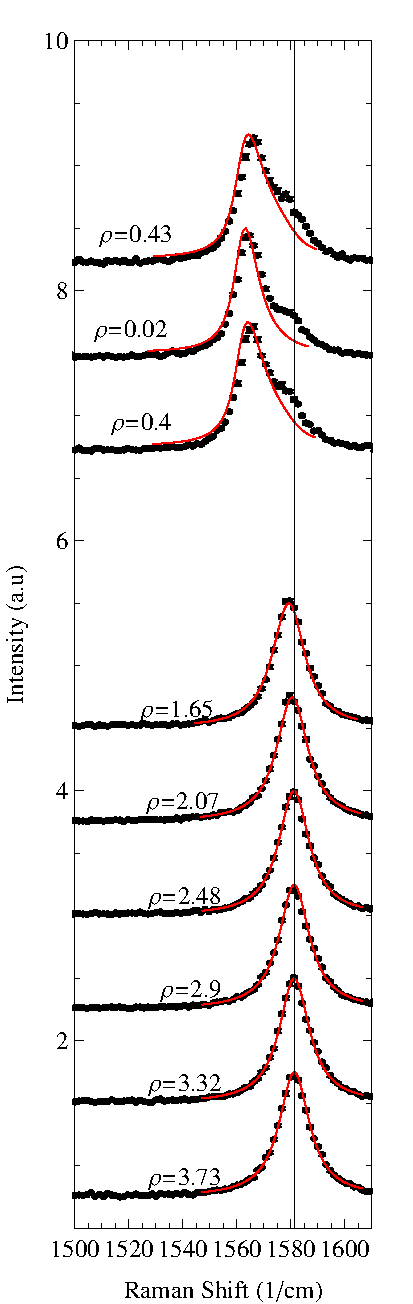
\includegraphics[scale=.675]{Figs_Friction/2012-12-18_Fit_101psi_Spectra_for_paper_sb04-6b.pdf}};
	
	%The picture of the hole
	\newcommand{\arrowlength}{.144*2.4 cm}%.144 is 2.5 um
	\begin{scope}[xshift=-.5 cm,yshift=1.25 cm]
		%For the total scale=1 the .jpg scale is .6
		\node at (0,0) {
\includegraphics[scale=.30375,angle=-90]{Figs_Friction/SB04-6b.jpg}};%was .225 before I change the scale from .5 to .45
		\draw[->,black,>=stealth] (-.03cm,-\arrowlength-.05 cm-.136 cm) -- +(0,2*\arrowlength);
	\end{scope}
\end{tikzpicture}
	\end{center}
	\caption{\label{fig:fri:igouter} Global fitting details for microchambers with radii less than 1.2 microns. Raman spectra from a line scan over a $\sim 1.2 \ \mu m$ radius bilayer sealed microchamber with 0.80 MPa of applied absolute pressure. The spectra taken along the path shown in the lower left inset are arrayed vertically with those spectra that were too close to the edge of the hole to be fit omitted.  The black vertical line is positioned at the supported graphene's unstrained G band energy.  The value of the sliding friction was found by fitting the spectra of the supported graphene ($\rho>1$) only.  Plotted in red are the spectra predicted by our extended Hencky model using the best fit to the sliding friction.  Even though they were not included in the fit, the spectra predicted by the extended Hencky model matches the major feature of the suspended spectra. }
\end{figure}

Unlike the sliding friction, the Gr\"{u}neisen parameter and shear deformation potential should be the same for every line scan
As such, they were included as fitting parameters only in the two lines scans which best defined the shear deformation potential based on the splitting of the supported graphene's G band just outside the edge of the microchamber: the $\sim 5 \mu m$ radius monolayer and the $\sim 5 \mu m$ radius trilayer at 0.80 MPa of applied pressure.
The best fit values, $\gamma=1.89 \pm 0.01$ and $\beta=0.70 \pm 0.04$, were then treated as known material parameters for the rest of the twenty full Raman line scans.
Figure \ref{fig:fri:gammabeta} details the extraction of these parameters.
Table \ref{tab:fri:gb} summarizes the measurements of the Gr\"{u}neisen parameter and shear deformation potentials of other research groups as well as their substrates.
Our measured $\gamma$ is commensurate with most of the other measured values and agrees particularly well with the \textit{ab initio} calculations of Cheng \emph{et al.}\cite{Cheng2011}.
On the other hand, our measured shear deformation potential is lower than most other measurements.
Buckling out-of-plane cannot explain this result since the mono and trilayers would buckle differently for a microchamber with the same pressure and radius.
To our knowledge, these are the first measurements of $\gamma$ and $\beta$ for which the sliding of FLG over its substrate was included.

\begin{figure}
	\begin{center}
	\newcommand{\sscale}{.8}
\begin{tikzpicture}[scale=\sscale]	
	\begin{scope}[xshift=-4.5 cm,yshift=0 cm]
		\node at (0,0) {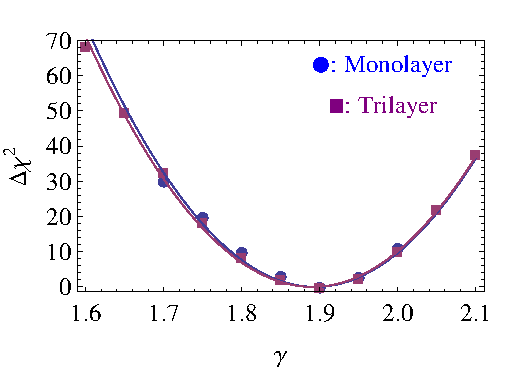
\includegraphics[scale=\sscale]{Figs_Friction/2012-12-11_Gbest.pdf}};
		\node at (-3.8,3) {\textbf{(a)}};
	\end{scope}
	
	\begin{scope}[xshift=4.5 cm,yshift=0 cm]
		\node at (0,0) {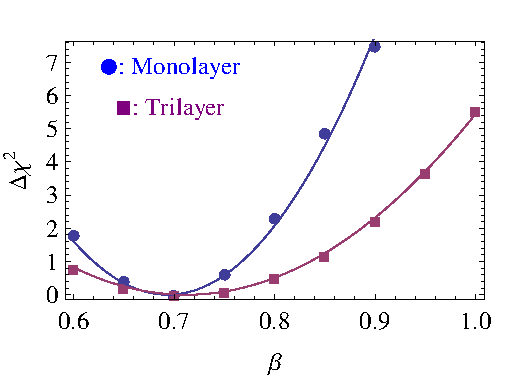
\includegraphics[scale=\sscale]{Figs_Friction/2012-12-11_Bbest.pdf}};
		\node at (-3.8,3) {\textbf{(b)}};
	\end{scope}
\end{tikzpicture}
	\end{center}
	\caption{\label{fig:fri:gammabeta}Determination of the Gr\"{u}neisen parameter and shear deformation potential. Global fits to a monolayer covered and a trilayer covered $\sim 5 \ \mu m$ radius sealed microchamber at 0.80 MPa of applied absolute pressure are used to determine the Gr\"{u}neisen parameter, $\gamma$, and shear deformation potential, $\beta$. The plotted circles and squares represent the increase of $\chi^2$ per degree of freedom away from the minimum value of the fit with the other fitting parameters ($\beta$ and $f$ for $\gamma$, and $\gamma$ and $f$ for $\beta$) chosen to minimize $\chi^2$ at each data point. The plotted curves represent a parabolic fit to the data. Using an increase in $\chi^2$ per degree of freedom of 0.25 gives: $\gamma_{mono} = 1.89 \pm .02$, $\gamma_{tri} = 1.89 \pm .02$, $\beta_{mono} = 0.69 \pm .04$, and $\beta_{tri} = 0.71 \pm .06$. The averages of the monolayer and the trilayer give $\gamma=1.89 \pm .01$ and $\beta= 0.70 \pm .04$.}
\end{figure}

\begin{table}
	\begin{center}
	\begin{tabular}{l c  c }
		\hline
		\hline
		 & $\gamma$ & $\beta$ \\
		 \hline
		 This work & 1.89 & .70 \\
		 $\mathrm{SiO_2}$ depression\cite{Metzger2010} & 2.4 & \\
		 On PDMS\cite{Huang2009} & .69 & .38 \\
		 On SU8\cite{Mohiuddin2009} & 1.99 & .99\\
		 Embedded\cite{Frank2010} & 2.01 & 1.01 \\
		 On Acrylic\cite{Yoon2011} & 2.2 & .93\\
		 Bubble\cite{Zabel2012} & 1.8 \\
		\textit{Ab initio} \cite{Thomsen2002} & 2.0 & 0.66 \\
		\textit{Ab initio} \cite{Cheng2011} & 1.86 & .96\\
		 \hline
		 \hline
	\end{tabular}
	\end{center}
	\caption{\label{tab:fri:gb} Summary of the Gr\"{u}neisen parameter, $\gamma$, and shear deformation potential, $\beta$, as measured on different substrates}
\end{table}

Figure \ref{fig:fri:fitlinescan} shows a global data fit for a $\sim 5 \ \mu m$ radius monolayer covered graphene sealed microchamber at 0.80 MPa of applied pressure.
The spectra and fits from each position along the line scan are stacked vertically in the direction of the line scan.
Our extended continuum model successfully fits the softening and splitting of the G band of the supported graphene and successfully predicts the downshift and sharpening of the G band of the suspended graphene as the center of the microchaber is approached.
In comparison, without our theoretical extension the standard Hencky model would fail to reproduce the supported graphene spectra.

\begin{figure}
	\begin{center}
	\begin{tikzpicture}[scale=.75]
	%The spectra
	\node at (0,0) {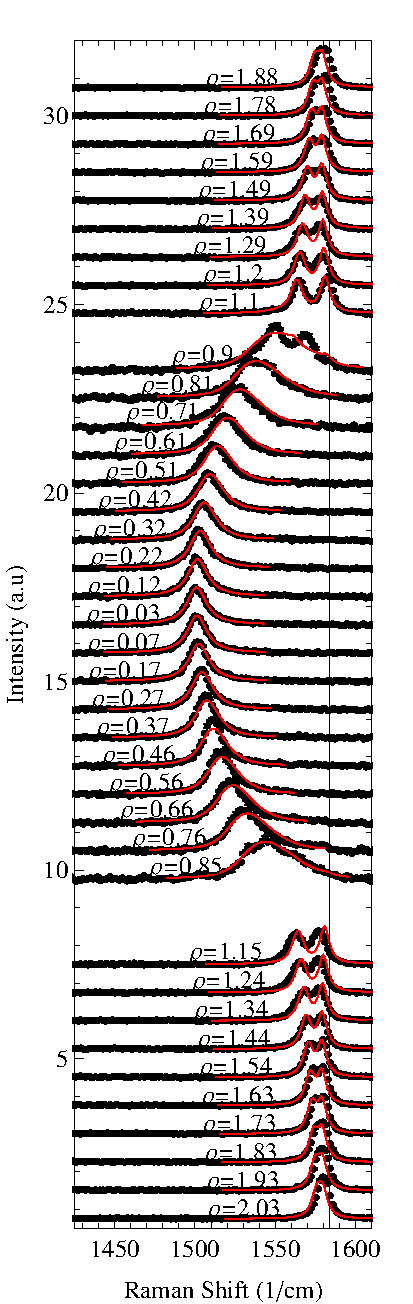
\includegraphics[scale=.75]{Figs_Friction/2012-12-18_Fit_101psi_Spectra_for_paper.pdf}};
	
	%The picture of the hole
	\newcommand{\arrowlength}{.44*1.2*1.77 cm}
	\begin{scope}[xshift=1.7 cm,yshift=.7 cm]
		%For the total scale=1 the .jpg scale is .6
		\node at (0,0) {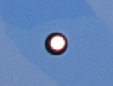
\includegraphics[scale=.8,angle=-90,trim=9.5mm 8.5mm 9.5mm 8.75mm,clip]{Figs_Friction/SB02_1_cropped.jpg}};
		\draw[->,black,thick,>=stealth] (0,-\arrowlength) -- (0,\arrowlength);
	\end{scope}
\end{tikzpicture}]
	\end{center}
	\caption{\label{fig:fri:fitlinescan} Raman spectra from a line scan over a $\sim 5 \ \mu m$ radius monolayer graphene sealed microchamber with 0.80 MPa of applied pressure analyzed with our extended Hencky model (red lines).  The spectra taken along the path shown in the inset are arrayed vertically with spectra taken too close to the edge of the microchamber omitted (see text).  The black vertical line is positioned at the supported graphene's unstrained G band energy.}
\end{figure}

\section{Measured frictional dependencies}
The sliding friction extracted for eight microchambers with radii between 1.2 and 5 $\mu m$ and with applied absolute pressures from 0.10 to 0.80 MPa exhibits fundamentally different behavior for trilayer graphene than for monolayer and bilayer.
In Figure \ref{fig:fri:FvsP}a (left) the friction is plotted as a function of pressure and the data for trilayer graphene (black dots) shows a linear dependence of the sliding friction vs applied pressure in accordance with Amontons' law with a coefficient of friction of $0.11 \pm 0.01$ as shown in Figure \ref{fig:fri:trimu}.
The sliding friction for monolayer and bilayer graphene decreases generally with applied pressure and the wide scatter of the points for different radii and layer number clearly indicate that the sliding friction is dependent on the geometry of the microchamber.
Our theoretical analysis shows that the radial strain at the edge due to the pressure pushing the graphene into the microchamber has the same radii and layer number dependence as the friction, so we replot the sliding friction as a function of the radial strain in Figure \ref{fig:fri:FvsP}b (right).
The monolayer and bilayer data for all different radii microchambers now \emph{collapse} to a single curve versus radial strain, well described by $1/\epsilon_{r,edge}$ behavior (dashed line). 

\begin{figure}
	\begin{center}
	\begin{tikzpicture}[scale=.9]
	%The spectra
	\node at (0,0) {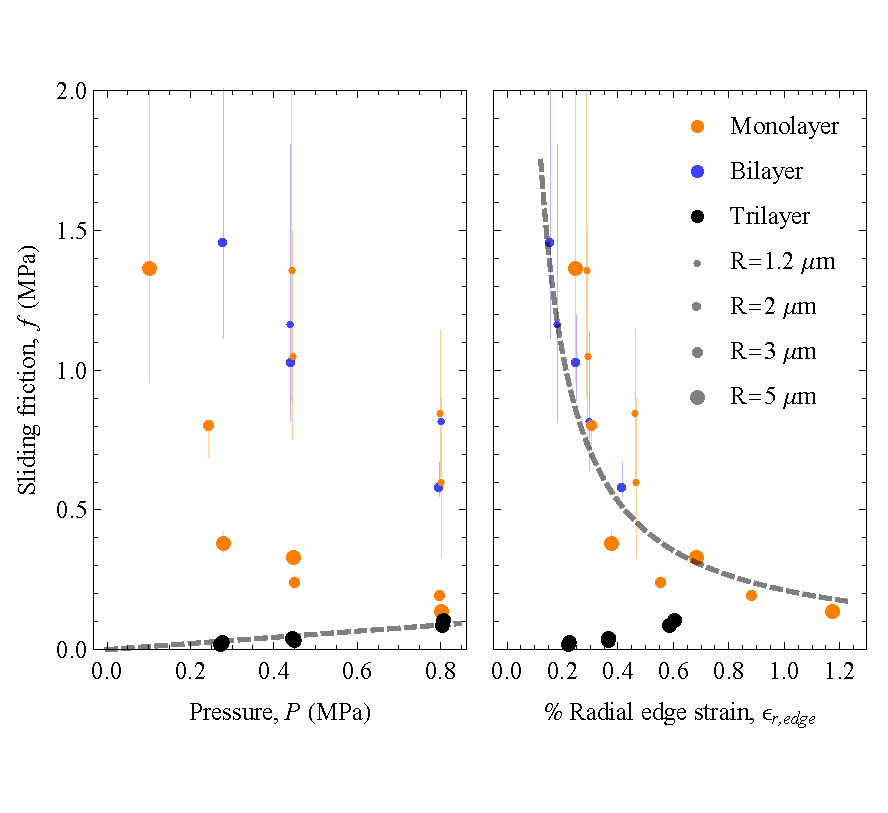
\includegraphics[scale=.9]{Figs_Friction/FvsP.pdf}};
	\node at (-5.8,5.75) {\textbf{a}};
	\node at (.95,5.75) {\textbf{b}};
\end{tikzpicture}
	\end{center}
	\caption{\label{fig:fri:FvsP}  Sliding friction, extracted by analyzing Raman G band line scans with our extended Hencky model, plotted as a function of absolute applied pressure in panel \textbf{a} (left) and as a function of the radial strain at the edge of the microchamber in panel \textbf{b} (right) for 5 different graphene sealed microchambers.  The size of each data point represents the radius of the FLG-sealed microchamber corresponding to that point. The error bars are given by an increase in global fit $\chi^2$ per degree of freedom of 0.25.  The sliding friction of trilayer graphene depends linearly on the absolute applied pressure in agreement with Amontons' law. The sliding friction of monolayer and bilayer graphene, however, go as the inverse of the radial strain at the edge of the microchamber.  Gray dashed lines are the best fits to these trends.}
\end{figure}

\begin{figure}
	\begin{center}
	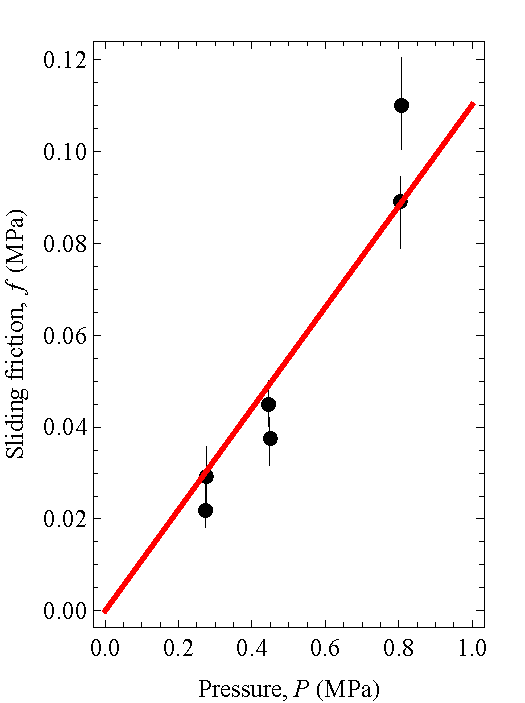
\includegraphics{Figs_Friction/Tri_mu.pdf}
	\end{center}
	\caption{\label{fig:fri:trimu} Determination of the coefficient of friction for trilayer graphene on silicon dioxide.  The sliding frictions extracted from Raman G band lines scans over two $5 \ \mu m$ radii trilayer sealed microchambers as a function of the absolute applied pressure is fit with Amonton's law, $f=\mu P_{abs}$, giving a coefficient of friction between trilayer graphene and $\mathrm{SiO_2}$ of $\mu=0.11 \pm 0.01$. For reference, Teflon on Teflon has $\mu=0.04$ while clean steel on clean steel has $\mu=0.6$\cite{Resnick2002}.}
\end{figure}

The gross difference in behavior between trilayer on one hand, and mono-and bilayer on the other, illustrates the two roles of the applied pressure.
The pressure load pushes the graphene more firmly onto the substrate so that sliding friction should increase (Amontons' law), yielding a positive coefficient of friction.
This is the case for the trilayer graphene.
On the other hand, as the pressure pushes the graphene into the microchamber, it creates a radial tension in the supported graphene outside the microchamber.
The data collapse in Figure \ref{fig:fri:FvsP}b for monolayer and bilayer graphene demonstrate that the pressure dependence of the sliding friction is not due to loading the supported graphene but is instead due to the graphene being pulled and stretched by the applied pressure.
This is the only mechanism that would depend on the geometric parameters of the microchamber while also being consistent with the data.
It is not surprising that the sliding friction for mono- and bilayer graphene is dependent on the strain and not the load because thin graphene conforms nearly perfectly to a $\mathrm{SiO_2}$ substrate\cite{Stolyarova2007,Lui2009,Cullen2010}.
Increasing the load cannot further increase the contact area, but increasing the radial strain beyond the edge of the microchamber may act to smooth out the graphene sheet, decreasing the contact between the graphene and the substrate, and thus decreasing the sliding friction.
The bending rigidity, which goes as thickness cubed, of trilayer graphene must be high enough to counteract the adhesion energy, causing lower conformation and allowing for a traditional pressure and load response.
The existence of a bilayer to trilayer crossover in FLG-substrate interactions is also observed in GPa range pressure measurements of silicon dioxide supported graphene\cite{Proctor2009,Nicolle2011}.
Nicolle \emph{et al.} observed a decrease in the pressure response of the G band between bilayer and trilayer graphene which was attributed to the transition from biaxial compression mediated by the substrate to hydrostatic compression mediated by the pressure transmitting medium\cite{Nicolle2011}.

\section{Summary}
In summary, we have shown that graphene slides along the substrate when pulled.
Furthermore, using a newly developed extension of the continuum Hencky model, we extracted the sliding friction as a function of the number of atomic layers and the load.
Trilayer graphene shows a typical load response whereas the sliding friction for monolayer and bilayer graphene goes as the inverse of strain.
The data collapse of the friction for mono- and bilayer graphene when plotted versus strain is strong experimental evidence for a reduction in surface conformation when graphene is pulled as the fundamental origin of the negative coefficient of friction.
These results will be important for the design of strain engineered devices\cite{Pereira2009a}, while the sliding of a flexible surface along a bulk object should be of fundamental, tribological interest.
Finally, the method used in generalizing Hencky's solution should be useful for including distributed strains in other continuum models for use in designing strain-engineered graphene devices and in understanding other, few-layer material systems.

	% Appendices
	\appendix 								% Appendices
	\chapter{The first Brillouin zone of strained graphene \label{chap:sBZ}}

In this appendix an approximate analytic expression for the positions of the corners of the first Brillouin zone in deformed graphene is presented.
The first Brillouin zone can then be constructed by connecting these points.
This proves useful in Chapter \ref{chap:PVP} to illustrate the distortion of reciprocal space that accompanies the distortion of graphene's lattice.
The strain dependence is found by applying a general method for determining the positions of the first Brillouin zone corners for close to hexaganal lattices.

The general method will follow the following steps:
\begin{enumerate}
	\item{The lattice vectors will be used to determine the reciprocal lattice vectors.}
	\item{The combination of reciprocal lattice vectors which give the important points in reciprocal space will be determined.}
	\item{The conditions for Bragg refraction will be used to determine the corners of the first Brillouin zone.}
\end{enumerate}
After establishing this general methodology, the explicit strain dependence can easily be determined to first order.

The lattice vectors $\vec{a}_+$ and $\vec{a}_-$ determine the reciprocal lattice vectors through the relationship $\vec{a}_i \cdot \vec{b}_j=2 \pi \delta_{ij}$ where $\vec{b}_j$ are the two reciprocal lattice vectors, $i$ and $j$ are $\in \{+,-\}$, and $\delta_{ij}$ is the Kronecker delta function \cite{Kittel2005}.
In two dimensions this implies the two matrix relationships which determine $\vec{b}_{\pm}$,
\begin{equation}
	\left(\begin{array}{cc}
		a_{\pm x} & a_{\pm y} \\
		a_{\mp x} & a_{\mp y} \end{array} \right)
	\left(\begin{array}{c} 
		b_{\pm x} \\
		b_{\pm y} \end{array} \right) 
	=
	\left(\begin{array}{c} 2 \pi \\ 0 \end{array} \right) \ .
	\label{eq:sBZ:RLVs}
\end{equation}
This orthogonality condition can be easily solved by inverting the matrix.
Having determined the form for the reciprocal lattice vectors, the next step is to determine the boundaries of the first Brillouin zone.

The traditional method of determining the first Brillouin zone is qualitatively simple, but not necessarily trivial to implement algorithmically.
In this method, one draws the perpendicular bisector of each reciprocal lattice vector given by $n \vec{b}_+ + m \vec{b}_-$ where $m$ and $n$ are integers.
The most inner polygon formed by the perpendicular bisectors is then the first Brillouin zone \cite{Kittel2005}.
The first step to simplify this method is to restrict the number of perpendicular bisectors which are considered.
The construction of the the first Brillouin zone for a perfect hexagonal lattice is shown in figure \ref{fig:sBZ:BZ}.
For clarity, the minimal set of reciprocal lattice vectors is shown.
None of the other reciprocal lattice vectors contribute a perpendicular bisector which is used in constructing the first Brillouin zone.
This set of six reciprocal lattice vectors is relatively robust to distortions of the hexagonal lattice.
They determine the first Brillouin zone for strains as large as 20 \% armchair uniaxial, 20 \% armchair uniaxial, or 20 \% shear strain.
Although the reciprocal lattice vectors themselves are different, their combinations remain the same.
This was confirmed by comparing the first Brillouin zone predicted by the method here with that calculated by geometric construction.
The phrase ``close to hexagonal'' lattices is used to refer to those lattice for which the minimal set of reciprocal lattice vectors is given by the combinations shown in figure \ref{fig:sBZ:BZ}.
For this discussion, the strained graphene lattice is then a close to hexagonal lattice.

\begin{figure}
	\begin{center}
	\newcommand{\blat}{2 cm}
\newcommand{\sqth}{1.73205080757}
\begin{tikzpicture}[>=stealth,
	RLV/.style={very thick,->,color=black},
	BZ/.style ={very thick, color=gray, dashed}]

	% The reciprocal lattice vectors that go to the 6 nearest neighbors
	\draw[RLV] (0,0) -- ( 30:\blat) node[anchor=south west]{$\vec{b}_+$};
	\draw[RLV] (0,0) -- ( 90:\blat) node[anchor=south     ]{$\vec{b}_+ + \vec{b}_-$};
	\draw[RLV] (0,0) -- (150:\blat) node[anchor=south east]{$\vec{b}_-$};
	\draw[RLV] (0,0) -- (210:\blat) node[anchor=north east]{$-\vec{b}_+$};
	\draw[RLV] (0,0) -- (270:\blat) node[anchor=north     ]{$-\vec{b}_+ - \vec{b}_-$};
	\draw[RLV] (0,0) -- (330:\blat) node[anchor=north west]{$-\vec{b}_-$};

	%The constructed first Brillouin zone
	\draw[BZ]
		(  0:\blat/\sqth) node[anchor=west      ]{$\bm{K_1} $} --
		( 60:\blat/\sqth) node[anchor=south west]{$\bm{K_3'}$} --
		(120:\blat/\sqth) node[anchor=south east]{$\bm{K_2}$} -- 
		(180:\blat/\sqth) node[anchor=east      ]{$\bm{K_1'}$} -- 
		(240:\blat/\sqth) node[anchor=north east]{$\bm{K_3}$} -- 
		(300:\blat/\sqth) node[anchor=north west]{$\bm{K_2'}$} -- 
		(  0:\blat/\sqth);

\end{tikzpicture}
	\end{center}
	\caption{\label{fig:sBZ:BZ} The construction of the first Brillouin zone for a hexagonal lattice.  The reciprocal lattice vectors which contribute the perpendicular bisectors that make up the first Brillouin zone are shown as labeled arrows. The dashed lines indicate the edge of the First Brillouin zone.  Close to hexagonal lattices are lattices for which the same set of reciprocal lattice vectors define the first Brillouin zone.}
\end{figure}

Having restricted the reciprocal lattice vectors, the corners of the first Brillouin zone can be constructed from the condition for Bragg reflection.
This condition,
\begin{equation*}
	\vec{k} \cdot \left(\frac{1}{2} \vec{G} \right)=\left(\frac{1}{2} \vec{G}\right)^2 \ ,
\end{equation*}
defines the wave vectors, $\vec{k}$, which make up the perpendicular bisector of the reciprocal lattice vector, $\vec{G}$ \cite{Kittel2005}.
If the wave vector is on the perpendicular bisector of two sequential reciprocal lattice vectors, then it is a corner of the first Brillouin zone.
For example, the corner $\bm{K}_1$ is a perpendicular bisector of both $-\vec{b}_-$ and $\vec{b_+}$.
Thus, the corners of the first Brillouin zone can be calculated analytically by using the matrix identity,
\begin{equation}
	\left(\begin{array}{cc}
		G_{1,x} & G_{1,y} \\
		G_{2,x} & G_{2,y} \end{array} \right)
	\left(\begin{array}{c} k_x \\ k_y \end{array} \right)
	=
	\left( \begin{array}{c} \frac{1}{2} G_1^2 \\ \frac{1}{2} G_2^2 \end{array} \right)
	\label{eq:sBZ:corners}
\end{equation}
where $\vec{G_1}$ and $\vec{G_2}$ are sequential reciprocal lattice vectors from Figure \ref{fig:sBZ:BZ}.
This matrix identity can be inverted to determine the wave-vector at the corner of the first Brillouin zone.
The full first Brillouin zone is given by the intersection of these corners.
This completes the general methodology for determining the first Brillouin zone based on the lattice vectors for close to hexagonal lattices.
In summary, the reciprocal lattice vectors are calculated from the lattice vectors using Equation \ref{eq:sBZ:RLVs} and then the corners of the first Brillouin zone can be found using Equation \ref{eq:sBZ:corners} for the reciprocal lattice vector combination shown in Figure \ref{fig:sBZ:BZ}.

The final step is to use the strain dependence of the lattice vectors given in Equation \ref{eq:PVP:StrainVectors} and approximate the result to first order in the elements of the displacement gradient tensor.
The first order approximation was found using Wolfram Mathematica version 9.0.
The first order strain dependence of the position of the corners of the first Brillouin zone are given by 
\begin{align*}
	\bm{K}_1&=-\bm{K'}_1\simeq 
		\frac{4 \pi}{3 \sqrt{3} a} \left( \begin{array}{cc} 1 \\ 0 \end{array} \right)
		+
		\frac{4 \pi}{3 \sqrt{3} a} \left( \begin{array}{cc}
		-\frac{1}{2} u_{xx}-\frac{1}{2}u_{yy} \\
		-\frac{1}{2} u_{yx} - \frac{3}{2} u_{xy}
		\end{array} \right) \\
	\bm{K}_2&=-\bm{K'}_2\simeq 
		\frac{4 \pi}{3 \sqrt{3} a} \left( \begin{array}{cc} -\frac{1}{2} \\ \frac{\sqrt{3}}{2} \end{array} \right)
		+
		\frac{4 \pi}{3 \sqrt{3} a} \left( \begin{array}{cc}
		u_{xx}-\frac{1}{2}u_{yy}-\frac{\sqrt{3}}{2} u_{yx} \\
		-\frac{\sqrt{3}}{2} u_{yy}-\frac{1}{2}u_{yx}
		\end{array} \right) 	\\
	\bm{K}_3&=-\bm{K'}_3\simeq 
		\frac{4 \pi}{3 \sqrt{3} a} \left( \begin{array}{cc} -\frac{1}{2} \\ -\frac{\sqrt{3}}{2} \end{array} \right)
		+
		\frac{4 \pi}{3 \sqrt{3} a} \left( \begin{array}{cc}
		u_{xx}-\frac{1}{2}u_{yy}+\frac{\sqrt{3}}{2} u_{yx} \\
		\frac{\sqrt{3}}{2}u_{yy}-\frac{1}{2} u_{yx}
		\end{array} \right) \ .
\end{align*}
The shifts in the corners of the first Brillouin zone are opposite for time reversal pairs respecting time reversal symmetry.
As should be expected for something that depends on the strained lattice vectors, the positions of the corners are determined by the terms of the displacement gradient tensor and not the strain tensor.
These approximation were tested against the geometric construction successfully.
They are used in Chapter \ref{chap:PVP} to visualize the distortion of Reciprocal space which accompanies the deformation of the real space lattice.
In particular, Figure \ref{fig:PVP:PVPshifts} shows the shifts in the corners of the first Brillouin zone for several deformation geometries.
	\chapter{Slowly varying approximation \label{chap:idep}}

A full, rigorous treatment of a non-uniform strain field is not compatible with the pseudo vector potential interpretation of strain developed in Chapter \ref{chap:TB}.
In a strict treatment of non-uniform strain the $i$ dependencies of Equation \ref{eq:TB:beforeSV} cannot be neglected and the transformation into Fourier space is obstructed.
Without elimination of the spatial dependence, the Hamiltonian of the full system must be painstakingly solved.
For properly engineered strain distributions, this would result in a dispersion relationship which exhibits Landau like levels.
Although rigorous, this method is more arduous and also less conceptually pleasing.
The pseudo vector potential approach provides a qualitative framework for understanding the observed effects.

In the slowly varying approximation the $i$ dependencies in Equation \ref{eq:TB:beforeSV} are eliminated.
This is as if the the strain is treated as locally uniform.
In this Appendix this approximation will be developed and the limits of validity will be discussed.

Remembering that $\bm{\nabla u}$ is $i$ dependent, the $i$ dependent terms in Equation \ref{eq:TB:beforeSV} are 
\begin{align*}
  H_i=&\sum_i \left( t_0+\delta t_{i,j} \right) e^{i(\vec{k}-\vec{k}')\cdot \vec{R}_i'}
  		e^{-i \vec{k}' \cdot \vec{\Delta}_{i,j}'} \\
  	 =&\sum_i \left( t_0+\delta t_{i,j} \right) e^{i(\vec{k}-\vec{k}')\cdot \vec{R}_i'}
  		e^{-i \vec{k}' \cdot (\bm{1}+\bm{\nabla u}) \vec{\Delta}_j} \\
  	 \simeq & e^{-i \vec{k}' \cdot \vec{\Delta}_j} \sum_i \left( t_0+\delta t_{i,j} \right)
  	 	e^{i(\vec{k}-\vec{k}')\cdot \vec{R}_i'} \left(1-i \vec{k}' \cdot \bm{\nabla u} \cdot \vec{\Delta}_j \right) \\
  	 \simeq & e^{-i \vec{k}' \cdot \vec{\Delta}_j} \bigg \{
  	 	t_0 \sum_i e^{i(\vec{k}-\vec{k}')\cdot \vec{R}_i'} 
  	 	-i t_0 \vec{k}' \cdot \sum_i \left( \bm{\nabla u} \ e^{i(\vec{k}-\vec{k}')\cdot \vec{R}_i'} \right) \cdot \vec{\Delta}_j
  	 	+\sum_i \delta t_{i,j} \  e^{i(\vec{k}-\vec{k}')\cdot \vec{R}_i'}
  	 	\bigg \} \\
  	 =& N t_0 \delta_{\vec{k},\vec{k}'}
  	 	-i t_0 \vec{k}' \cdot \widetilde{\bm{\nabla u}}_{\vec{k}-\vec{k}'} \cdot \vec{\Delta}_j + \widetilde{\delta t}_{\vec{k}-\vec{k}'} \ ,
\end{align*}
where $\widetilde{\bm{\nabla u}}_{\vec{k}-\vec{k}'}$ and $\widetilde{\delta t}_{\vec{k}-\vec{k}'}$ are the Fourier transforms of $\delta t_{i,j}$ and $\bm{\nabla u}$ respectively.
Only terms first order in products of the small quantities $\bm{\nabla u}$ and $\delta t_{i,j}$ were kept.
All of the $i$ dependence has been absorbed by the Fourier transforms.

Only specific Fourier components yield relevant $\widetilde{\bm{\nabla u}}_{\vec{k}-\vec{k}'}$ and $\widetilde{\delta t}_{\vec{k}-\vec{k}'}$ when working in the low energy regime.
The wave-vectors will again be approximated as $\vec{k}=\bm{K}+\vec{q}$ and $\vec{k}=\bm{K'}+\vec{q}$ with the additional small parameter $qa$, giving
\begin{align*}
  \widetilde{\delta t}_{\vec{k}-\vec{k}'} &=
    \sum_i \delta t_{i,j} e^{i(\bm{K^{(')}}+\vec{q}-\bm{K^{(')}}-\vec{q}') \cdot \vec{R}_i'} \\
                              &\simeq 
    \sum_i \delta t_{i,j} e^{i(\bm{K^{(')}}-\bm{K^{(')}}) \cdot \vec{R}_i'} (1+(\vec{q}-\vec{q}') \cdot \vec{R}_i') \\
                              &=
    \sum_i \delta t_{i,j} e^{i(\bm{K^{(')}}-\bm{K^{(')}}) \cdot \vec{R}_i'} \ ,
\end{align*}
where $\bm{K^{(')}}$ refers to either $\bm{K}$ or $\bm{K'}$ depending on the wave-vector.
The low energy approximation for $\widetilde{\bm{\nabla u}}_{\vec{k}-\vec{k}'}$ is identical.
Thus, to first order in the small parameters the only relevant Fourier components are for $\vec{k}-\vec{k}' \in \{0,\bm{K}-\bm{K'}, \bm{K'}-\bm{K} \}$.
The high frequency components could interestingly act to couple the $\bm{K}$ and $\bm{K}'$ points.
However, here we apply the slowly varying approximation for which we eliminate the high frequency components and limit $\vec{k}-\vec{k}' \rightarrow 0$, yielding
\begin{align*}
  \widetilde{\delta t}_{\vec{k}-\vec{k}'}     & \simeq N \delta_{\vec{k},\vec{k}'} ( <\delta t_{i,j}>) \\
  \widetilde{\bm{\nabla u}}_{\vec{k}-\vec{k}'}& \simeq N \delta_{\vec{k},\vec{k}'} ( <\bm{\nabla u} >) \ .
\end{align*}
where $<\delta t_{i,j}>=\delta t_j$ and $<\bm{\nabla u}>$ are the average value over $i$ of $\delta t_{i,j}$ and $\bm{\nabla u}$ respectively.

Thus, in the slowly varying approximation the $i$ dependence of Equation \ref{eq:TB:beforeSV} becomes
\begin{equation*}
	H_i=N \delta_{\vec{k},\vec{k}'}  \left( t_0 + \delta t_j - i t_0 \vec{k}' \cdot \bm{\nabla u} \cdot \vec{\Delta}_j \right)
\end{equation*}
which gives the same result as the simple substitutions $\delta t_{i,j} \rightarrow \delta t_j=<\delta t_{i,j}>$ and $\bm{\nabla u}_i \rightarrow <\bm{\nabla u}>$ in Equation \ref{eq:TB:beforeSV}.
This approximation required low energies, $qa<<1$, small strains, $\delta t_j << t_0$ $\bm{\nabla u}<<1$, and slowly varying strain fields, $\widetilde{\delta t}_{\bm{K}-\bm{K}'}=\widetilde{\bm{\nabla u}}_{\bm{K}-\bm{K}'}=0$.
It eliminates of the spatial dependence in the Hamiltonian of strained graphene allowing the identification of the pseudo vector potential.

	% Bibliography
	\backmatter
	\begin{singlespace}						% Bibliography can be single spaced
		\bibliographystyle{apalike}			% Should be listed alphabetically
		\bibliography{thesis}
	\end{singlespace}

	%CV at end--probably the absolute last thing to tack on
\end{document}